%-----------------------------------------------------------------
%	BASIC DOCUMENT LAYOUT
%-----------------------------------------------------------------
\documentclass[paper=a4, fontsize=12pt, twoside=semi]{scrartcl}
\usepackage[T1]{fontenc}
\usepackage[utf8]{inputenc}
\usepackage{lmodern}
\usepackage{slantsc}
\usepackage{microtype}
\usepackage[catalan]{babel}
\usepackage[backend=bibtex, style=trad-abbrv, sorting=none, maxbibnames=2]{biblatex}
\addbibresource{bibliografia.bib}
\makeatletter
	\def\blx@maxline{77}
\makeatother

% Sectioning layout
\addtokomafont{sectioning}{\normalfont\scshape}
\usepackage{tocstyle}
\usetocstyle{standard}
\renewcommand*\descriptionlabel[1]{\hspace\labelsep\normalfont\bfseries{#1}}

% Empty pagess
\usepackage{etoolbox}
\pretocmd{\section}{\cleardoubleevenemptypage}{}{}
\pretocmd{\part}{\cleardoubleevenemptypage\thispagestyle{empty}}{}{}
\renewcommand\partheadstartvskip{\clearpage\null\vfil}
\renewcommand\partheadmidvskip{\par\nobreak\vskip 20pt\thispagestyle{empty}}

% Paragraph indentation behaviour
\setlength{\parindent}{0pt}
\setlength{\parskip}{0.3\baselineskip plus2pt minus2pt}
\newcommand{\sk}{\medskip\noindent}

% Fancy header and footer
\usepackage{fancyhdr}
\pagestyle{fancyplain}
\fancyhead[LO]{\thepage}
\fancyhead[CO]{}
\fancyhead[RO]{\nouppercase{\mytitle}}
\fancyhead[LE]{\nouppercase{\leftmark}}
\fancyhead[CE]{}
\fancyhead[RE]{\thepage}
\fancyfoot{}
\renewcommand{\headrulewidth}{0.3pt}
\renewcommand{\footrulewidth}{0pt}
\setlength{\headheight}{13.6pt}

%-----------------------------------------------------------------
%	MATHS AND SCIENCE
%-----------------------------------------------------------------
\usepackage{amsmath,amsfonts,amsthm,amssymb}
\usepackage{xfrac}
\usepackage[a]{esvect}
\usepackage{chemformula}
\usepackage{graphicx}

\usepackage[arrowdel]{physics}
	\renewcommand{\vnabla}{\vec{\nabla}}
	% \renewcommand{\vectorbold}[1]{\boldsymbol{#1}}
	% \renewcommand{\vectorarrow}[1]{\vec{\boldsymbol{#1}}}
	% \renewcommand{\vectorunit}[1]{\hat{\boldsymbol{#1}}}
	\renewcommand{\vectorarrow}[1]{\vec{#1}}
	\renewcommand{\vectorunit}[1]{\hat{#1}}
	\renewcommand*{\grad}[1]{\vnabla #1}
	\renewcommand*{\div}[1]{\vnabla \vdot \va{#1}}
	\renewcommand*{\curl}[1]{\vnabla \cp \va{#1}}
	\let\rot\curl

% SI units
\usepackage[separate-uncertainty=true, alsoload=astro, alsoload=hep]{siunitx}
\sisetup{range-phrase = \text{--}, range-units = brackets}
\DeclareSIPrePower\quartic{4}
	\DeclareSIUnit\C{C}
	\DeclareSIUnit\dyn{dyn}
	\DeclareSIUnit\erg{erg}
	\DeclareSIUnit\year{y}
	\DeclareSIUnit\atm{atm}
	\DeclareSIUnit\cal{cal}
	\DeclareSIUnit\torr{torr}
	\DeclareSIUnit\au{AU}
	\DeclareSIUnit\jansky{Jy}
	\DeclareSIUnit\esu{esu}
	\DeclareSIUnit\planck{\textit{h}}
	\DeclareSIUnit\Msun{\textit{M}_{\odot}}
	\DeclareSIUnit\Lsun{\textit{L}_{\odot}}
	\DeclareSIUnit\Rsun{\textit{R}_{\odot}}

% Smaller trig functions
\newcommand{\Sin}{\trigbraces{\operatorname{s}}}
\newcommand{\Cos}{\trigbraces{\operatorname{c}}}
\newcommand{\Tan}{\trigbraces{\operatorname{t}}}

% Operator-style notation for matrices
\newcommand*{\mat}[1]{\hat{#1}}

% Matrices in (A|B) form via [c|c] option
\makeatletter
\renewcommand*\env@matrix[1][*\c@MaxMatrixCols c]{%
  \hskip -\arraycolsep
  \let\@ifnextchar\new@ifnextchar
  \array{#1}}
\makeatother

% Shorter \mathcal and \mathbb
\newcommand*{\mc}[1]{\mathcal{#1}}
\newcommand*{\mbb}[1]{\mathbb{#1}}

% Shorter ^\ast and ^\dagger
\newcommand*{\sast}{^{\ast}{}}
\newcommand*{\sdag}{^{\dagger}{}}

%-----------------------------------------------------------------
%	OTHER PACKAGES
%-----------------------------------------------------------------
\usepackage{environ}

%Left numbered equations
\makeatletter
	\NewEnviron{Lalign}{\tagsleft@true\begin{align}\BODY\end{align}}
\makeatother

% Plots and graphics
\usepackage{pgfplots}
\usepackage{tikz}
\usepackage{color}
	\makeatletter
		\color{black}
		\let\default@color\current@color
	\makeatother

% Richer enumerate, figure, and table support
\usepackage{enumerate}
\usepackage[shortlabels]{enumitem}
\usepackage{float}
\usepackage{tabularx}
\usepackage{booktabs}
	% \setlength{\intextsep}{8pt}
\numberwithin{equation}{section}
\numberwithin{figure}{section}
\numberwithin{table}{section}

% No indentation after certain environments
\makeatletter
\newcommand*\NoIndentAfterEnv[1]{%
	\AfterEndEnvironment{#1}{\par\@afterindentfalse\@afterheading}}
\makeatother
% \NoIndentAfterEnv{thm}
\NoIndentAfterEnv{defi}
\NoIndentAfterEnv{example}
\NoIndentAfterEnv{table}

% Misc packages
\usepackage{ccicons}
\usepackage{lipsum}

%-----------------------------------------------------------------
%	THEOREMS
%-----------------------------------------------------------------
\usepackage{thmtools}

% Theroems layout
\declaretheoremstyle[
	spaceabove=6pt, spacebelow=6pt,
	headfont=\normalfont,
	notefont=\mdseries, notebraces={(}{)},
	bodyfont=\small,
	postheadspace=1em,
]{small}

\declaretheorem[style=plain,name=Teorema,qed=$\square$,numberwithin=section]{thm}
\declaretheorem[style=plain,name=Corol·lari,qed=$\square$,sibling=thm]{cor}
\declaretheorem[style=plain,name=Lema,qed=$\square$,sibling=thm]{lem}
\declaretheorem[style=definition,name=Definició,qed=$\blacksquare$,numberwithin=section]{defi}
\declaretheorem[style=definition,name=Exemple,qed=$\blacktriangle$,numberwithin=section]{example}
\declaretheorem[style=small,name=Demostració,numbered=no,qed=$\square$]{sproof}

%-----------------------------------------------------------------
%	ELA MOTHERFUCKING GEMINADA
%-----------------------------------------------------------------
\def\xgem{%
	\ifmmode
		\csname normal@char\string"\endcsname l%
	\else
		\leftllkern=0pt\rightllkern=0pt\raiselldim=0pt
		\setbox0\hbox{l}\setbox1\hbox{l\/}\setbox2\hbox{.}%
		\advance\raiselldim by \the\fontdimen5\the\font
		\advance\raiselldim by -\ht2
		\leftllkern=-.25\wd0%
		\advance\leftllkern by \wd1
		\advance\leftllkern by -\wd0
		\rightllkern=-.25\wd0%
		\advance\rightllkern by -\wd1
		\advance\rightllkern by \wd0
		\allowhyphens\discretionary{-}{}%
		{\kern\leftllkern\raise\raiselldim\hbox{.}%
			\kern\rightllkern}\allowhyphens
	\fi
}
\def\Xgem{%
	\ifmmode
		\csname normal@char\string"\endcsname L%
	\else
		\leftllkern=0pt\rightllkern=0pt\raiselldim=0pt
		\setbox0\hbox{L}\setbox1\hbox{L\/}\setbox2\hbox{.}%
		\advance\raiselldim by .5\ht0
		\advance\raiselldim by -.5\ht2
		\leftllkern=-.125\wd0%
		\advance\leftllkern by \wd1
		\advance\leftllkern by -\wd0
		\rightllkern=-\wd0%
		\divide\rightllkern by 6
		\advance\rightllkern by -\wd1
		\advance\rightllkern by \wd0
		\allowhyphens\discretionary{-}{}%
		{\kern\leftllkern\raise\raiselldim\hbox{.}%
			\kern\rightllkern}\allowhyphens
	\fi
}

\expandafter\let\expandafter\saveperiodcentered
	\csname T1\string\textperiodcentered \endcsname

\DeclareTextCommand{\textperiodcentered}{T1}[1]{%
	\ifnum\spacefactor=998
		\Xgem
	\else
		\xgem
	\fi#1}

%-----------------------------------------------------------------
%	PDF INFO AND HYPERREF
%-----------------------------------------------------------------
\usepackage{hyperref}
\usepackage{cleveref}
\hypersetup{colorlinks, citecolor=black, filecolor=black, linkcolor=black, urlcolor=black}

\newcommand*{\mytitle}{Introducció a l'astrofísica}
\newcommand*{\mysubtitle}{}
\newcommand*{\myauthor}{Diego Pavón Coloma}
\newcommand*{\myuni}{Universitat Autònoma de Barcelona, Departament de Física}
% \newcommand*{\mydate}{\normalsize 2014-2015} % My year
\newcommand*{\mydate}{\normalsize 2016-2017} % Apunts Pavón

\pdfstringdefDisableCommands{\def\and{i }}

\usepackage{hyperxmp}
\hypersetup{pdfauthor={Alfredo Hernández Cavieres}, pdftitle={\mytitle}}

%-----------------------------------------------------------------
%	TITLE SECTION AND DOCUMENT BEGINNING
%-----------------------------------------------------------------
\newcommand{\horrule}[1]{\rule{\linewidth}{#1}}
\title{
	\normalfont
	\small \scshape{\myuni} \\ [25pt]
	\horrule{0.5pt} \\[0.4cm]
	\huge \mytitle \\
	% \Large \scshape{\mysubtitle} \\
	\horrule{2pt} \\[0.5cm]
}
\author{\myauthor}
\date{\mydate}

\begin{document}

\clearpage\maketitle
\thispagestyle{empty}
\addtocounter{page}{-1}

%-----------------------------------------------------------------
%	LICENCE
%-----------------------------------------------------------------
\section*{}\thispagestyle{empty}
\begin{centering}
	\href{http://creativecommons.org/licenses/by-nc-sa/4.0/deed.ca}{\huge \ccbyncsaeu}

	\normalsize Aquesta obra està subjecta a una llicència de

	Reconeixement-NoComercial-CompartirIgual 4.0

	Internacional de Creative Commons.

	\phantom{blindtext}

	Edició i traducció per Alfredo Hernández Cavieres

	S'agrairia que informéssiu d'errors i correccions a \href{mailto:alfredoignacio.hernandez@e-campus.uab.cat}{\nolinkurl{alfredoignacio.hernandez@e-campus.uab.cat}}

\end{centering}

%-----------------------------------------------------------------
%	DOCUMENT BODY
%-----------------------------------------------------------------
\cleardoubleevenemptypage
\pdfbookmark[1]{\contentsname}{toc}
\tableofcontents

\setcounter{secnumdepth}{0}
%-----------------------------------------------------------------
%	CONSTANTS I FACTORS DE CONVERSIÓ
%	!TEX root = ./../main.tex
%-----------------------------------------------------------------
\section{Constants i factors de conversió}
\subsection*{Constants universals\footnote{Per raons històriques, a l'astrofísica és estàndard fer servir el sistema CGS (\textit{centimetre--gram--second}) d'unitats.}}
\begin{itemize}[leftmargin=*]
	\item Velocitat e la llum al buit: $c = \SI{3 e 10}{\cm \per \s}$.
	\item Permitivitat al buit: $\varepsilon_{0} = \SI{8.854 e -12}{\square\C \per \newton \per \square\metre}$.
	\item Permeabilitat al buit: $\mu_{0} = \SI{4\pi e -7}{\m\kg \per \square\C}$.
	\item Constant de gravitació: $G = \SI{6.67 e-8}{\dyn \square\cm \per \square\g}$.
	\item Constant de Planck: $h = \SI{6.626 e -27}{\erg \s} = \SI{4.134 e-15}{\eV \s}$.
	\item Constant de Planck reduïda: $\hbar \equiv h/(2\pi) = \SI{1.055 e -27}{\erg \s} = \SI{6.579 e-16}{\eV \s}$.
	\item Constant d'estructura fina: $\alpha = \si{\elementarycharge\squared \per \planckbar \per \clight} \approx \num{1/137.036}$.
\end{itemize}

%-----------------------------------------------------------------
\subsection*{Constants atòmiques}
\begin{itemize}[leftmargin=*]
	\item Càrrega de l'electró: $e = \SI{1.602 e-19}{\C} = \SI{4.803 e-10}{\esu}$.
	\item Constant de Boltzmann: $k_{B} = \SI{1.381 e-16}{\erg \per \K} = \SI{8.617 e-5}{\eV \per \K}$.
	\item Constant dels gasos: $R \equiv k_{B}/N_{A} = \SI{8.314}{\J \per \K \per \mol} = \SI{0.082}{\atm \litre \per \K \per \mol}$.
	\item Nombre d'Avogadro: $N_{A} = \SI{6.022 e23}{\per\mol}$.
	\item Constant d'Stefan--Boltzmann: $\sigma = \SI{5.670 e-5}{\erg \per \square\cm \per \s \per \quartic\K}$.
	\item Constant de radiació: $a \equiv \pi^{2}k_{B}^{4}/(15c^3\hbar^{3}) = \SI{7.566 e-15}{\erg \per \cubic\cm \per \quartic\K}$.
	\item Secció eficaç de Thomson: $\sigma_{T} \equiv 8\pi e^4/(3m_{e}^2c^4) = \SI{6.652 e-25}{\cm^{2}}$.
	\item Radi de Bohr: $a_{0} \equiv \hbar^{2}/(m_{e}e^{2}) = \SI{5.292 e-9}{\cm}$.
	\item Longitud d'ona de Compton de l'electró: $\lambda_{c} \equiv \hbar/(m_{e}c) = \SI{2.426 e-14}{\cm}$.
\end{itemize}

%-----------------------------------------------------------------
\subsection*{Masses atòmiques}
\begin{itemize}[leftmargin=*]
	\item Massa de l'electró: $m_{e} = \SI{9.109 e-28}{\g} = \SI{0.511}{\mega \eVperc \squared}$.
	\item Massa del protó: $m_{p} = \SI{1.673 e-24}{\g} = \SI{938.272}{\mega \eVperc \squared}$.
	\item Massa del neutró: $m_{n} = \SI{1.675 e-24}{\g} = \SI{939.56}{\mega \eVperc \squared}$.
	\item Massa del deuteró: $m_{d} = \SI{1875.612}{\eVperc \squared}$.
	\item Massa de la partícula alfa: $m(\ch{^{4}_{2}H}) = \SI{1.225}{\giga \eVperc \squared}$.
	\item Massa de l'àtom d'hidrogen: $m_{H} = \SI{938.386}{\mega \eVperc \squared}$.
	\item Massa atòmica: $\si{\amu} \equiv m(\ch{^{12} C}) =  \SI{931.494}{\mega \eVperc \squared}$.
	% \item Massa del deuteró: $m_{d} = \SI{3.344 e-24}{\g} = \SI{1875.612}{\eVperc \squared}$.
	% \item Massa de la partícula alfa: $m(\ch{^{4}_{2}H}) = \SI{6.646 e-24}{\g} = \SI{1.225}{\giga \eVperc \squared}$.
	% \item Massa de l'àtom d'hidrogen: $m_{H} = \SI{1.673 e-24}{\g} = \SI{938.386}{\mega \eVperc \squared}$.
	% \item Massa atòmica: $\si{\amu} \equiv m(\ch{^{12} C}) = \SI{1.66054 e-24}{\g} = \SI{931.494}{\mega \eVperc \squared}$.
\end{itemize}

%-----------------------------------------------------------------
\subsection*{Constants astronòmiques}
\begin{itemize}[leftmargin=*]
	\item Massa del Sol: $M_{\odot} = \SI{1.988 e33}{\g}$.
	\item Radi del Sol: $R_{\odot} = \SI{6.955 e10}{\cm}$.
	\item Lluminositat del Sol: $L_{\odot} = \SI{3.846 e33}{\erg\per\s}$.
	\item Constant solar: $F_{\odot} = \SI{1.360 e6}{\erg \per\s \per\square\cm}$.
	\item Temperatura de la superfície solar: $T_{\odot} = \SI{5780}{\K}$.
	\item Magnitud absoluta del Sol: $M_{\odot} = \num{4.76}$.
	\item Massa de la Terra: $M_{\oplus} = \SI{5.972 e 27}{\g}$.
	\item Radi de la Terra: $R_{\oplus} = \SI{6.367 e8}{\cm}$.
	\item Massa de la Lluna: $M_{L} = \SI{7.346 e 25}{\g}$.
	\item Radi de la Lluna: $R_{L} = \SI{1.738 e8}{\cm}$.
	\item Constant de Hubble: $H_{0} = \SI{100}{\planck \km \per \s \per \mega\parsec}$, on $h \in [0.5,0.9]$.
	\item Temps de Hubble: $H_{0}^{-1} = \SI{3.086 e17}{\per \planck \s} = \SI{9.778}{\per \planck \giga \year}$.
	\item Radi de Hubble: $c H_{0}^{-1} = \SI{2997.9}{\per \planck \mega \parsec}$.
	% Note that h in here is not planck's constant, but the expansion rate. I use it here for pure convenience.
\end{itemize}

%-----------------------------------------------------------------
\subsection*{Unitats de Planck}
\begin{itemize}[leftmargin=*]
	\item Massa de Planck: $M_{Pl} = \sqrt{\hbar c / G} \approx \SI{2.2 e-5}{\g}$.
	\item Longitud de Planck: $l_{Pl} = \sqrt{\hbar G / c^{3}} \approx \SI{1.6 e-33}{\cm}$.
	\item Temps de Planck: $t_{Pl} = \sqrt{\hbar G / c^{5}} \approx \SI{5.4 e-44}{\s}$.
	\item Temperatura de Planck: $T_{Pl} = \sqrt{\hbar c^{5}/ G} / k_{B} \approx \SI{1.4 e32}{\K}$.
\end{itemize}

%-----------------------------------------------------------------
\subsection*{Constants numèriques}
\begin{itemize}[leftmargin=*]
	\item Pi: $\pi = \num{3.141593}$.
	\item Nombre d'Euler: $e = \num{2.718282}$.
	\item Constant d'Euler--Mascheroni: $\gamma = \num{0.577216}$.
	\item Zeta de Riemann: $\zeta(3) = \num{1.202057}$.
	\item Logaritmes: $\ln 10 = \num{2.302585}$, $\log e = \num{0.434294}$, $\log 2 = \num{0.301030}$, $\log 3 = \num{0.477121}$.
\end{itemize}

%-----------------------------------------------------------------
\subsection*{Factors de conversió}
\begin{itemize}[leftmargin=*] %\item $\SI{1}{} = \SI{}{}$.
	\item $\SI{1}{\eV} = \SI{1.602 e-12}{\erg}$.
	\item $\SI{1}{\erg} = \SI{1}{\dyn \cm} = \SI{6.242 e11}{\eV} = \SI{e-7}{\J}$.
	\item $\SI{1}{\dyn} = \SI{e-5}{\N}$.
	\item $\SI{1}{\cal} = \SI{4.184}{\J}$.
	\item $\SI{1}{\J} = \SI{0.239}{\cal}$.
	\item $\SI{1}{\esu} = \SI{3.336 e-10}{\coulomb}$.
	\item $\SI{1}{\atm} = \SI{1.013 e5}{\Pa} = \SI{760}{\mmHg}$.
	\item $\SI{1}{\bar} = \SI{e5}{\Pa}$.
	\item $\SI{1}{\torr} = \SI{1}{\mmHg} = \SI{133.3}{\Pa}$.
	\item $\SI{1}{\kg} = \SI{5.610 e29}{\mega \eVperc \squared}$.
	\item $\SI{1}{\mega \eVperc \squared} = \SI{1.783 e-27}{\g}$.
	\item $\SI{1}{\amu} = \SI{1.66054 e-27}{\kg} = \SI{931.494}{\mega \eVperc \squared}$.
	\item $\SI{1}{\parsec} = \SI{3.262}{\lightyear} = \SI{2.063e5}{\au} = \SI{3.086 e18}{\cm}$.
	\item $\SI{1}{\lightyear} = \SI{9.461 e17}{\cm}$.
	\item $\SI{1}{\au} = \SI{1.496 e13}{\cm}$.
	\item $\SI{1}{\year} = \SI{3.1558149984 e7}{\s}$.
	\item $\SI{1}{\arcsecond} = \SI{4.848 e-6}{\radian}$.
\end{itemize}


\setcounter{secnumdepth}{2}
%-----------------------------------------------------------------
%	INTRODUCTION
%	!TEX root = ./../main.tex
%-----------------------------------------------------------------
\section{Introduction}
\subsection{Lorentz classical model}
In this model (figure \ref{fig:lorentz-model}), the force that acts upon the electron is modelled as a recovery force:
\begin{align}
	\va{F} = - k \va{r} \, \overset{1D}{\longmapsto} \, F = - k x
\end{align}
\begin{figure}[H]
	\centering
	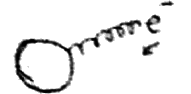
\includegraphics[width=0.2\textwidth]{./images/1-lorentz-model}
	\caption{Diagram of the Lorentz model for an atom}
	\label{fig:lorentz-model}
\end{figure}

Therefore, the equation of motion for the electron is
\begin{align*}
	\ddot{x} + \omega_{0}^{2}x = 0 \qc \omega_{0} = \sqrt{\frac{k}{m}} \Rightarrow x = A \cos(\omega_{0} t + \varphi)
\end{align*}
Introducing a damping term to account for the spontaneous emission, we get
\begin{align}
	\ddot{x} + \gamma \dot{x} + \omega_{0}^{2}x = 0
\end{align}

%-----------------------------------------------------------------
\subsection[Electric dipole approximation]{Electric dipole approximation (EDA)}
In the presence of an external electric field, $\va{E}(z,t) = E_{0} \cos(kz - \omega t) \vu{x}$, and introducing the oscillator strength, $f$, we can explain absorption and stimulated emission as well.

\begin{defi}[Oscillator strength]
	The oscillator strength, $f$, is a dimensionless quantity that expresses the probability of absorption or emission of electromagnetic radiation in transitions between energy levels of an atom or molecule.
	\begin{align*}
		f &> 0 \Rightarrow \text{ absorption} \\
		f &< 0 \Rightarrow \text{ stimulated emission}
	\end{align*}
\end{defi}

The force that acts upon a charged particle in the presence of an electric field is $\va{F} = q \va{E}$, therefore, we get
\begin{align*}
	\ddot{x} + \gamma \dot{x} + \omega_{0}^{2}x = f \frac{e E_{0}}{m} \cos(kz - \omega t)
\end{align*}

We can assume that the size of the atom is much smaller than the optical wavelength, so that the electron only sees the field at the nuclear position; this approximation is the so called electric dipole approximation. Therefore, $k z_{cm} \to 0$, and the previous equation becomes
\begin{align}
	\ddot{x} + \gamma \dot{x} + \omega_{0}^{2}x = f \frac{e E_{0}}{m} \cos(\omega t)
\end{align}

Consequently, we can get absorption or stimulated emission. Since $\dv*{W}{t} = - P$, we can study them measuring the mean value of the power in a cycle:
\begin{align}
	\ev{P} = \ev{F \dot{x}}
	\begin{cases}
		>0 & \text{(absorption)} \\
		<0 & \text{(stimulated emission)}
	\end{cases}
\end{align}
This models gives us $x(t)$.

\subsubsection*{Susceptibility}
In a homogeneous linear and isotropic dielectric medium, the polarization is aligned with and proportional to the electric field: $\va{P} = \varepsilon_{0} \chi \va{E}$. In a dipole, it can be written as $P = N e x$. Therefore, we can express the susceptibility as
\begin{align}
	\chi = \frac{N e x}{\varepsilon E} \equiv \chi' + i \chi''
\end{align}
The real part of the susceptibility, $\Re{\chi} = \chi'$ is related to index of refraction of the medium; the imaginary part, $\Im{\chi} = \chi''$ is related to the absorption coefficient.

\subsubsection*{Other media}
The natural frequency, $\omega_{0}$, gives us the model of the properties of the media. For metals, for instance, $\omega_{0} \to 0$ (electrons are not bound).

%-----------------------------------------------------------------
\subsection{Classical coherence}
\subsubsection*{First-order correlation function}
We can measure the coherence of an electric field with the help of an interferometer. In the figure \ref{fig:interferometer}, we see that $\va{E}_{1} = \va{E}(t)$, $\va{E}_{2} = \va{E}(t + \tau)$, and $\va{E}_{sum} = \va{E}_{1} + \va{E}_{2}$. So that, the intensity detected is $I \propto \ev{\va{E}^{2}_{sum}}$.
\begin{figure}[H]
	\centering
	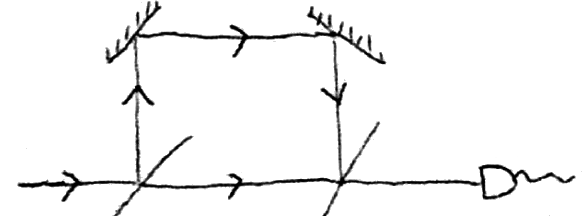
\includegraphics[width=0.5\textwidth]{./images/1-interferometer}
	\caption{Diagram of an interferometer with 50--50 beam splitters}
	\label{fig:interferometer}
\end{figure}

If we express $\va{E}(\va{r},t) = \va{E}^{(-}(\va{r},t) + \va{E}^{(-}(\va{r},t)$, where $\va{E}^{(+)} \equiv \va{E}^{(-)\sast}$, we can rewrite the expression for $I$:
\begin{flalign*}
	I & \propto \ev{(\va{E}_{1} + \va{E}_{2})^{2}} = \cdots = \ev{E^{(-)}_{1} E^{(+)}_{1}} + \ev{E^{(-)}_{2} E^{(+)}_{2}} + 2 \Re{ \ev{E^{(-)}_{1} E^{(+)}_{2}} } & \\
	& \Rightarrow I \propto 2 I_{0} + 2 \Re{E^{(-)}(t) + E^{(+)}(t + \tau)}
\end{flalign*}

\begin{defi}[First-order correlation function]
	\begin{align}
		G^{(1)}(t, t + \tau) \equiv \ev{E^{(-)}(t) + E^{(+)}(t + \tau)} = G^{(1)}(\tau)
	\end{align}
\end{defi}

The visibility is defined as $V = \dfrac{I_{max} - I_{min}}{I_{max} + I_{min}}$. Rewriting the first-order correlation function as $G^{(1)}(\tau) = \abs{G^{(1)}(\tau)} e^{i \phi(\tau)}$, we can easily work out $I_{max}$ and $I_{min}$:
\begin{flalign*}
	I & \propto 2 I_{0} + 2 \abs{G^{(1)}(\tau)} \cos[\phi(\tau)] \Rightarrow
	\begin{cases}
		I[\cos(\phi)] = -1 \Leftrightarrow I_{min} = 2I_{0} - 2 \abs{G^{(1)}(\tau)} \\
		I[\cos(\phi)] = +1 \Leftrightarrow I_{max} = 2I_{0} + 2 \abs{G^{(1)}(\tau)}
	\end{cases}
	 &
\end{flalign*}

\begin{defi}[Normalised first-order coherence function]
	We can rearrange the terms of the visibility to express it in terms of the first-order coherence function:
	\begin{align*}
		V = \dfrac{\abs{G^{(1)}(\tau)}}{\ev{E^{(-)}(t) E^{(+)}(t)}}
	\end{align*}
	this is what we call the normalised first-order coherence function, $g^{(1)}(\tau)$.
	\begin{align}
		V = \frac{I_{max} - I_{min}}{I_{max} + I_{min}} = \abs{g^{(1)}(\tau)}
		\begin{cases}
			= 0 & \Rightarrow \text{incoherent field} \\
			\in (0,1) & \Rightarrow \text{partially coherent field} \\
			= 1 & \Rightarrow \text{fully coherent field}
		\end{cases}
	\end{align}
\end{defi}

\subsubsection*{Second-order correlation function}
\begin{defi}[Normalised second-order correlation function]
	The degree of second-order correlation function is the autocorrelation function for the intensity, rather than the field. We can define this function as
	\begin{align}
		g^{(2)}(\tau) = \frac{\ev{ E^{(-)}(t) E^{(-)}(t + \tau) E^{(+)}(t + \tau) E^{(+)}(t) }}{\ev{ E^{(-)}(t) E^{(+)}(t) }}
	\end{align}
\end{defi}

%-----------------------------------------------------------------
\subsection{Hanbury--Brown--Twiss experiment}
One important feature of the second-order coherence function is that it can be measured with a reasonably simple set-up, the famous Hanbury--Brown–-Twiss apparatus (figure \ref{fig:hbt-experiment}). An input field is divided by a beam splitter, and the two components are monitored by two photo-detectors. The two detector signals are fed into a signal multiplier (mixer), though only after a variable time delay is added to one of the signals. The mixer signal is fed through a low-pass filter, which can be thought of as a integrator with a running time average.
\begin{figure}[H]
	\centering
	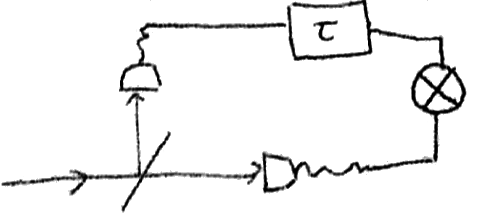
\includegraphics[width=0.4\textwidth]{./images/1-hbt-experiment}
	\caption{Diagram fo the Hanbury--Brown--Twiss experiment}
	\label{fig:hbt-experiment}
\end{figure}
This set-up, because it effectively correlates the two intensities, seems to give the $g^{(2)}(\tau)$ function as its output signal directly:
\begin{align}
	g^{(2)}(\tau) = \frac{\ev{I(t) I(t + \tau)}}{\ev{I(t)}^{2}}
\end{align}

\begin{align*}
	g^{(2)}(\tau)
	\begin{cases}
		\text{stationary field} & g^{(2)} (\tau) = 1 \\
		\text{fluctuating field} &
		\begin{cases}
			g^{(2)} (0) \geq 1 \\
			g^{(2)} (\tau) \leq g^{(2)} (0)
		\end{cases}
		\Rightarrow \text{bunching}
	\end{cases}
\end{align*}

\begin{figure}[H]
	\centering
	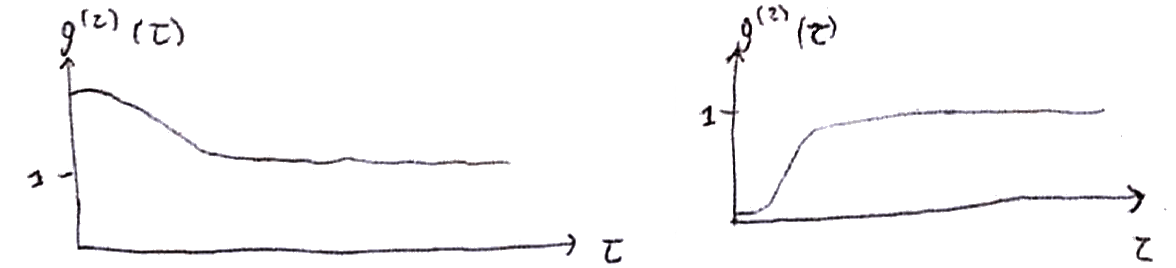
\includegraphics[width=\textwidth]{./images/1-bunching}
	\caption{(a) Bunching in a classical field, (b) antibunching in a quantum field}
	\label{fig:bunching}
\end{figure}

%-----------------------------------------------------------------
%	ESCALA DE MAGNITUDS ESTEL·LARS
%	!TEX root = ./../main.tex
%-----------------------------------------------------------------
\section{Escala de magnituds estel·lars}
\subsection{Escala de magnituds estel·lars}
% FIXME: hipparcus@sec:bio
Hiparc de Rodes ($\approx$ 190--120 aC) va assignar magnitud aparent $m = 1$ a l'estrella més brillant del firmament i, descendent, $m=6$ a la menys brillant (a simple vista).

\subsubsection*{Fotòmetre}
És un instrument ideat per mesurar la brillantor d'una estrella. Quan la llum d'aquesta incideix sobre una superfície foto-sensible es crea un corrent per efecte fotoelèctric. La llum rebuda al telescopi passa, a través d'un filtre, a una superfície sensible a la llum coneguda com a càtode. El càtode emet electrons que són multiplicats per un foto-multiplicador, de tal manera que el senyal és fàcilment mesurable. Cada fotó detectat pel càtode genera un pols; el nombre de polsos per segon és proporcional a la brillantor de l'estrella. En fotometria d'alta velocitat els polsos són comptats en intervals molt més curts que 1 segon. Hi fotòmetres capaços de mesurar magnituds estel·lars amb un error màxim proper a la mil·lèsima de magnitud $m$.

\begin{defi}[Lluminositat, $L$]
	Energia emesa per una estrella per unitat de temps. Al CGS té unitats de $\qty[L] = \si{\erg\per\s}$.
\end{defi}

\begin{defi}[Flux radiant, $F$]
	Assumint que la llum no és absorbida durant el seu viatge al fotòmetre, el flux radiant mesurat a una distància $r$ està relacionat amb la lluminositat $L$ de l'estrella per
	\begin{align}
		F = \frac{L}{4\pi r^{2}}
	\end{align}
	que és l'energia rebuda per unitat d'àrea i de temps ($\si{\erg\per\square\cm\per\s}$).
\end{defi}

\begin{example}
	La lluminositat del Sol és $\Lsun = \SI{3.826 e33}{\erg \per \s}$, a la distància de $\SI{1}{\au} = \SI{1.496 e13}{\cm}$. Llavors, la Terra rep un flux radiant just per sobre de la seva atmosfera (que és absorbent):
	\begin{align*}
		F_{\odot} = \frac{\num{3.826 e33}}{4\pi (\num{1.496 e13})^{2}} = \SI{1.360 e6}{\erg \per \square\cm \per \s}
	\end{align*}
	Aquest valor s'anomena \textit{constant solar}.
\end{example}

\begin{defi}[Magnitud aparent, $m$]
	Siguin $F_{1}$ i $F_{2}$ els fluxos radiants rebuts de dues estrelles (suposant que no hi ha absorció), llavors la diferència en magnituds aparents es defineix com
	\begin{align}
		m_{1} - m_{2} = -2.5 \log(\frac{F_{1}}{F_{2}}) % \Leftrightarrow \frac{F_{2}}{F_{1}} = 100^{(m_{1}-m_{2})/5}
	\end{align}
	o bé
	\begin{align}
		\frac{F_{2}}{F_{1}} = 100^{(m_{1}-m_{2})/5}
	\end{align}
	La magnitud aparent $m$ depèn de $L$ i de $r$.
\end{defi}

\begin{defi}[Magnitud absoluta, $M$]
	És la magnitud aparent que tindria una estrella si estigués a $\SI{10}{\parsec}$ de nosaltres.
	\begin{align}
		100^{(m - M)/5} = \frac{F_{10}}{F} = \qty(\frac{d}{\SI{10}{\parsec}})^{2} \Rightarrow d = 10^{(m - M + 5)/5} \si{\parsec}
	\end{align}
\end{defi}

\begin{defi}[Distància mòdul, $\mu = m - M$]
	Dóna una indicació de la distància $d$ en què es troba una estrella de la Terra.
	\begin{align}
		m - M = 5 \log(\frac{d}{\SI{10}{\parsec}})
	\end{align}
\end{defi}

% \begin{example}
%     Sabent que la magnitud aparent del Sol (a $\SI{1}{\au}$ de la Terra) és $m_{\odot} = -26.81$, trobeu la seva magnitud absoluta.
%     \begin{align*}
%         \Msun & = m_{\odot} - 5 \log(\frac{d}{\SI{10}{\parsec}}) = 4.76
%     \end{align*}
% \end{example}

\begin{example}
	La magnitud absoluta d'una estrella a la Galàxia Andròmeda (a \SI{690}{\kilo \parsec} de nosaltres) és $M = 5$. L'estrella explota sobtadament donant lloc a una supernova de magnitud aparent $m = 6.7$. Trobeu: (a) el quocient entre les lluminositats intrínseques de la supernova, $L_{2}$, i l'estrella progenitora, $L_{1}$; (b) La magnitud absoluta de la supernova.
	\begin{Lalign}\tag{a}
	\begin{gathered}
		d = 10^{(m-M+5)/5} \si{\parsec} \Rightarrow m_{1} = -5 + M_{1} + 5 \log d = 29.19 \\
		m_{1} - m_{2} = -2.5 \log(\frac{F_{1}}{F_{1}}) \Rightarrow \log(\frac{L_{2}}{L_{1}}) = \frac{m_{1}-m_{2}}{2.5} = 8.99\\
		\Rightarrow \frac{L_{2}}{L_{1}} = 10^{8.99} \approx \num{9.9 e8}
	\end{gathered}
	\end{Lalign}
	\begin{Lalign}\tag{b}
		d &= 10^{(m-M+5)/5} \si{\parsec} \Rightarrow M_{2} = m_{2} + 5 - 5 \log d = -17.49
	\end{Lalign}
\end{example}

\begin{example}
	La magnitud aparent d'una sistema estel·lar triple és $m = 0.0$. Dues de les seves components posseeixen magnituds $m_{A} = 1.0$ i $m_{B} = 2.0$. Quina és la magnitud de la tercera component?
	\begin{align*}
		m - m_{0} = -2.5 \log(\frac{F}{F_{0}})
	\end{align*}
	Triem $m_{0} = 0$ (és a dir, $F_{0} = 1$), llavors
	\begin{align*}
		m = -2.5 \log F
	\end{align*}
	Trivialment trobem $F_{A}$ i $F_{B}$. Per una altra part, tenim que
	\begin{align*}
		m_{total} = -2.5 \log F_{total} = -2.5 \log (F_{A} + F_{B} + F_{C})
	\end{align*}
	Llavors,
	\begin{align*}
		m_{C} = -2.5 \log[F_{total} - (F_{A} + F_{B})] = 0.89
	\end{align*}
\end{example}

Si dues estrelles $A$ i $B$ es troben a la mateixa distància de la Terra, tindrem
\begin{align*}
	100^{(M_{A}-M_{B})/5} = \frac{L_{B}}{L_{A}}
\end{align*}
i si una de elles és el Sol, la magnitud absoluta de l'altra estrella serà
\begin{align}
	M = \Msun - 2.5 \log(\frac{F}{F_{10,\odot}})
\end{align}

Fins aquí hem considerat magnituds bolomètriques (totes les longituds de l'espectre visible) i hem menyspreat l'extinció i l'absorció. En general, es compleix
\begin{align}
	m_{\lambda} - M_{\lambda} = 5 \log(\frac{d}{\SI{10}{\parsec}}) + a_{\lambda}
\end{align}
on $a_{\lambda}$ és un factor de correcció que té en compte l'absorció a la longitud d'ona $\lambda$.

%-----------------------------------------------------------------
\subsection{Determinació de distàncies astronòmiques}
\subsubsection*{Polsos de radar}
\begin{figure}[H]
	\centering
	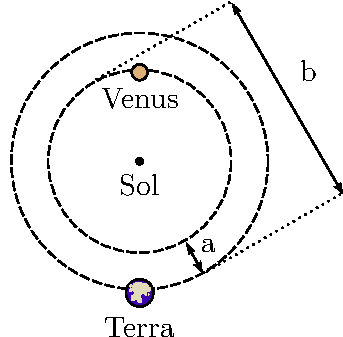
\includegraphics[width=0.3\textwidth]{./images/2-radar-venus-earth}
	\caption{Diagrama il·lustratiu del sistema Terra--Venus i les seves òrbites al voltant del Sol}
	\label{fig:radar}
\end{figure}

Mitjançant polsos de radar s'ha aconseguit trobar la distància a Venus\footnote{El semieix major de l'òrbita de Venus respecte el Sol és $\approx \SI{0.7233}{\au}$.} amb $\SI{\pm 1}{\km}$ de precisió. Un cop coneguda la distància a Venus quan està més a prop de la Terra, $a$, i quan està més lluny, $b$, es veu trivialment que la distància al Sol és
\begin{align*}
	d(\oplus, \odot) = \frac{a+b}{2} \equiv \SI{1}{\au} \approx \SI{1.496 e13}{\cm}
\end{align*}

\subsubsection*{Paral·laxi trigonomètrica}
És un mètode que s'utilitza per mesurar la distància a una estrella \textit{propera}. L'estrella és observada des d'extrems oposats de l'òrbita terrestre (6 mesos entre dues observacions successives) respecte el fons \textit{immòbil} d'estrelles.
\begin{figure}[ht]
	\centering
	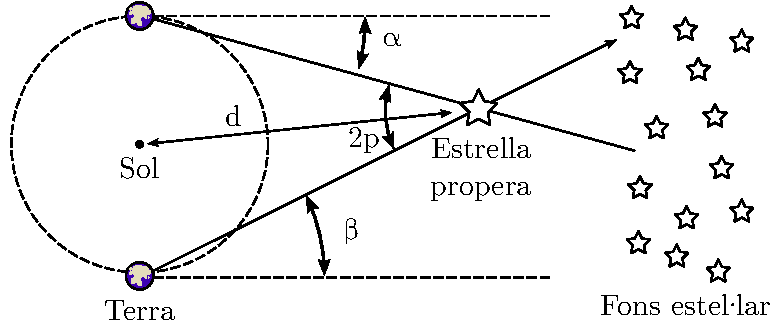
\includegraphics[width=0.7\textwidth]{./images/2-trig-parallax}
	\caption{Diagrama de l'observació de la posició relativa d'una estrella propera respecte el fons d'estrelles llunyanes}
	\label{fig:trig-parallax}
\end{figure}

\begin{align}
	p = \frac{1}{2} (\alpha + \beta) \Rightarrow d = \frac{1}{p\si{\arcsecond}}
\end{align}
Una estrella de paral·laxi $p = \SI{1}{\arcsecond}$ es troba a $\SI{1}{\parsec} \approx \SI{2.063 e5}{\au}$ (parsec) de distància de la Terra.

El satèl·lit \textit{Hipparcos} ha obtingut posicions de més de 120 mil estrelles amb gran precisió ($\sim \SI{e-3}{\arcsecond}$) fins a distàncies de $\SI{100}{\parsec}$ (això dota una precisió del $\SI{10}{\percent}$ a aquesta distància).

\subsubsection*{Paral·laxi espectroscòpica}
És un mètode que fa ús de les línies espectrals. Un cop coneguda la distància a les estrelles pròximes, es pot relacionar la seva brillantor absoluta, o lluminositat, amb el seu tipus espectral.

Astronòmicament les estrelles més brillants de cada tipus espectral es converteixen en indicadors de distància a distàncies tals que només les estrelles més brillants poden ser observades individualment (a tals distàncies la paral·laxi trigonomètrica ja no és útil).

\subsubsection*{Mètode del cúmul en moviment}
És un mètode vàlid per determinar la distància a un cúmul estel·lar (de mida $D \ll d$) els membres del qual són pròxims i es desplacen en grup.
\begin{figure}[ht]
	\centering
	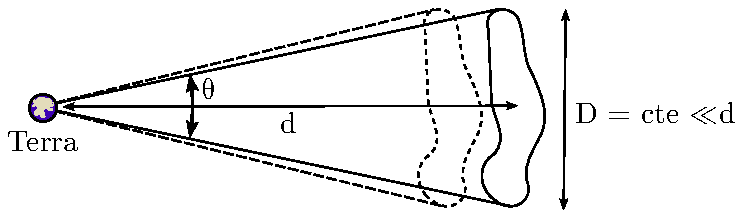
\includegraphics[width=0.7\textwidth]{./images/2-cluster-mov}
	\caption{Diagrama de l'observació d'un cúmul en moviment per determinar la seva distància}
	\label{fig:cluster-mov}
\end{figure}

\begin{align}
	\theta = \frac{D}{d} \Rightarrow \dot{\theta} = - D\frac{d}{d^{2}} \Rightarrow d = - v \frac{\theta}{\dot{\theta}}
\end{align}
La  velocitat $v$ del cúmul al llarg de la visual ve donada pel desplaçament Doppler de les línies espectrals; $\dot{\theta}$ es determina comparant la posició de les estrelles en plaques fotogràfiques preses amb desenes d'anys de diferència.

Aquest mètode només s'ha emprat amb èxit en la determinació de la distància al Cúmul de les Híades ($ \approx \SI{48}{\parsec}$).

\subsubsection*{Superposició de seqüències principals}
Es basa en la hipòtesi que les estrelles de la seqüència principal\footnote{A la pàgina \pageref{sec:hertz-russell} es fa un tractament més profund dels diagrames de Hertzsprung--Russell i el significat de la seqüència principal.} tenen idèntiques propietats amb independència del cúmul al qual pertanyen. Llavors, el pendent de la seqüència principal serà el mateix en tots els cúmuls i les estrelles de la seqüència principal del mateix tipus espectral o color tenen la mateixa magnitud absoluta independentment del cúmul.

Sota aquesta hipòtesi, podem comparar la lluminositat de les estrelles en la seqüència principal del Cúmul de les Híades amb les de qualsevol altre cúmul.

El desplaçament vertical per superposar ambdós cúmuls dóna la distància relativa entre ambdós cúmuls:
\begin{align}
	\Delta m \equiv m_{GC} - m_{Hya} = 5 \log(\frac{d_{GC}}{d_{Hya}}) + a'
\end{align}
on $a'$ és la correcció deguda a la diferència en l'enrogiment interestel·lar entre ambdós cúmuls; aquesta pot ser determinada per l'ús de les línies espectrals.

\subsubsection*{Estrelles RR Lyrae}
Un cert tipus d'estrelles grogues, gegants, polsants amb període d'oscil·lació entre 0.2 i 1.2 dies, i amb $0.2 \leq \Delta m \leq 2$ magnituds, són de la població II\footnote{Les estrelles de la població I contenen quantitats significatives d'elements més pesats que l'heli (anomenats genèricament \textit{metalls} en astrofísica). Aquests elements foren produïts per generacions anteriors d'estrelles a través d'explosions de supernova. El nostre Sol pertany al grup de població I. Són habituals als braços espirals de la Via Làctia. Les estrelles de la població II són les primeres estrelles de vida llarga formades després del Big Bang i, per tant, contenen poca quantitat de metalls. Es troben en cúmuls globulars i al centre de la Via Làctia. Evidentment, són estrelles molt més velles que les de la població I.} i es troben en l'halo de la galàxia i en cúmuls globulars.

La magnitud aparent, $m$, de totes les RR Lyrae variables resulta ser la mateixa en un cúmul donat (tot i que varia d'un cúmul a un altre), independentment del seu període. Ja que són intrínsecament lluminoses i el seu període les fa destacar, són indicadores ideals de distàncies.

Suposem que la magnitud absoluta, $M$, és la mateixa amb independència del cúmul. Així, la distància entre dos cúmuls pot determinar-se mitjançant la fórmula
\begin{align}
	\Delta m \equiv m_{1} - m_{2} = 5 \log(\frac{d_{1}}{d_{2}}) + a'
\end{align}

\subsubsection*{Estrelles variables Cefeides}
% FIXME: leavitt@sec:bio
Estrelles grogues, gegants o supergegants, de lluminositat variable observades per primer cop als Núvols de Magalhães (galàxies nanes del nostre Grup Local). La seva importància deriva de la relació (descoberta per Henrietta Leavitt) entre període i magnitud absoluta (al visible).
\begin{align}\label{eq:cepheid}
	M_{v} = (-2.43 \pm 0.12) (\log(T) - 1) - (4.05 \pm 0.02)
\end{align}
Llavors, observant el període coneixem la magnitud absoluta $M$, i mitjançant l'expressió
\begin{align}
	M = \Msun - 2.5 \log(\frac{L}{\Lsun})
\end{align}
determinem la seva lluminositat $L$. Coneguda $L$ i el seu flux lumínic que arriba a la Terra es troba la distància.
\begin{figure}[h]
	\centering
	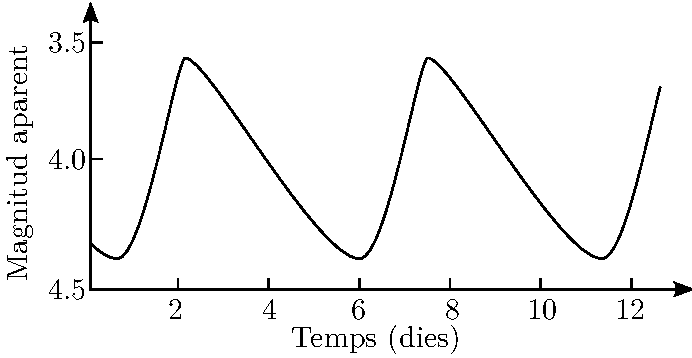
\includegraphics[width=0.6\textwidth]{./images/2-cepheid}
	\caption{Corba de llum de la Cefeida $\delta$--Cephei, amb magnitud variable $m$ (entre $\numrange{3.6}{4.3}$) en un període de 5.4 dies}
	\label{fig:cepheid}
\end{figure}

\subsubsection*{Noves}
La seva magnitud absoluta, $M$, està relacionada amb el ritme de decreixement de lluminositat després d'un \textit{outburst}. L'enorme lluminositat intrínseca d'una nova fa d'ella un indicador molt útil de distàncies en el cas de galàxies properes.

\subsubsection*{Supernoves}
S'han observat explosions de supernoves fins a distàncies corresponents a \textit{redshift} $z = 2$. La lluminositat de les supernoves pot determinar-se si es coneix (a través de l'observació) el ritme de decreixement de la seva lluminositat. Tanmateix, observacions a diferents longituds d'ona permeten calibrar l'extinció ocasionada per la pols interestel·lar, que podria conduir a una falsa estimació de la distància.

El primer registre d'una supernova és la Supernova Tycho (una de les vuit supernoves que han estat visibles a simple vista), observada pel famós astrònom Tycho Brahe l'11 de novembre de 1572 [\href{http://apod.nasa.gov/apod/ap990307.html}{APOD~990307}].

\subsubsection*{Relació Tully--Fisher}
Relació empírica entre l'amplada de la línia de $\SI{21}{\cm}$ de l'hidrogen neutre (\textit{spin-flip} d'electró--protó, $\Delta E = hc/\lambda = \SI{6 e-6}{\eV}$) a galàxies espirals (causada per la seva rotació) i la lluminositat:
\begin{align}
	\frac{L_{H}}{\num{3 e10} L_{H\odot}} \approx \qty[\frac{v_{\max}}{\SI{196}{\km\per\s}}]^{3.8}
\end{align}
Aquesta relació es pot utilitzar per determinar la distància relativa entre galàxies espirals així com entre grups de galàxies.

Ja que la matèria fosca contribueix notablement a $v_{\max}$ però no contribueix a la lluminositat, aquesta relació empírica és difícil d'entendre.

\subsubsection*{Relació entre la distància i els desplaçament cap al roig}
Observant els objectes més brillants de les galàxies (tals com estrelles O, noves, Cefeides variables, les quals poden ser detectades fins i tot en les galàxies més properes del Cúmul de Virgo) s'adverteix la relació empírica $z \propto d$, on $z$ es defineix com
\begin{align}
	z = \frac{\Delta \lambda}{\lambda} = \frac{\lambda_{obs} - \lambda_{em}}{\lambda_{em}}
\end{align}

Així, si una galàxia és observada a \textit{redshift} $z_{1}$ i una altra a $z_{2}$, la relació de distàncies entre elles serà
\begin{align}
	\frac{d_{1}}{d_{2}} = \frac{z_{1}}{z_{2}}
\end{align}
\begin{figure}[H]
	\centering
	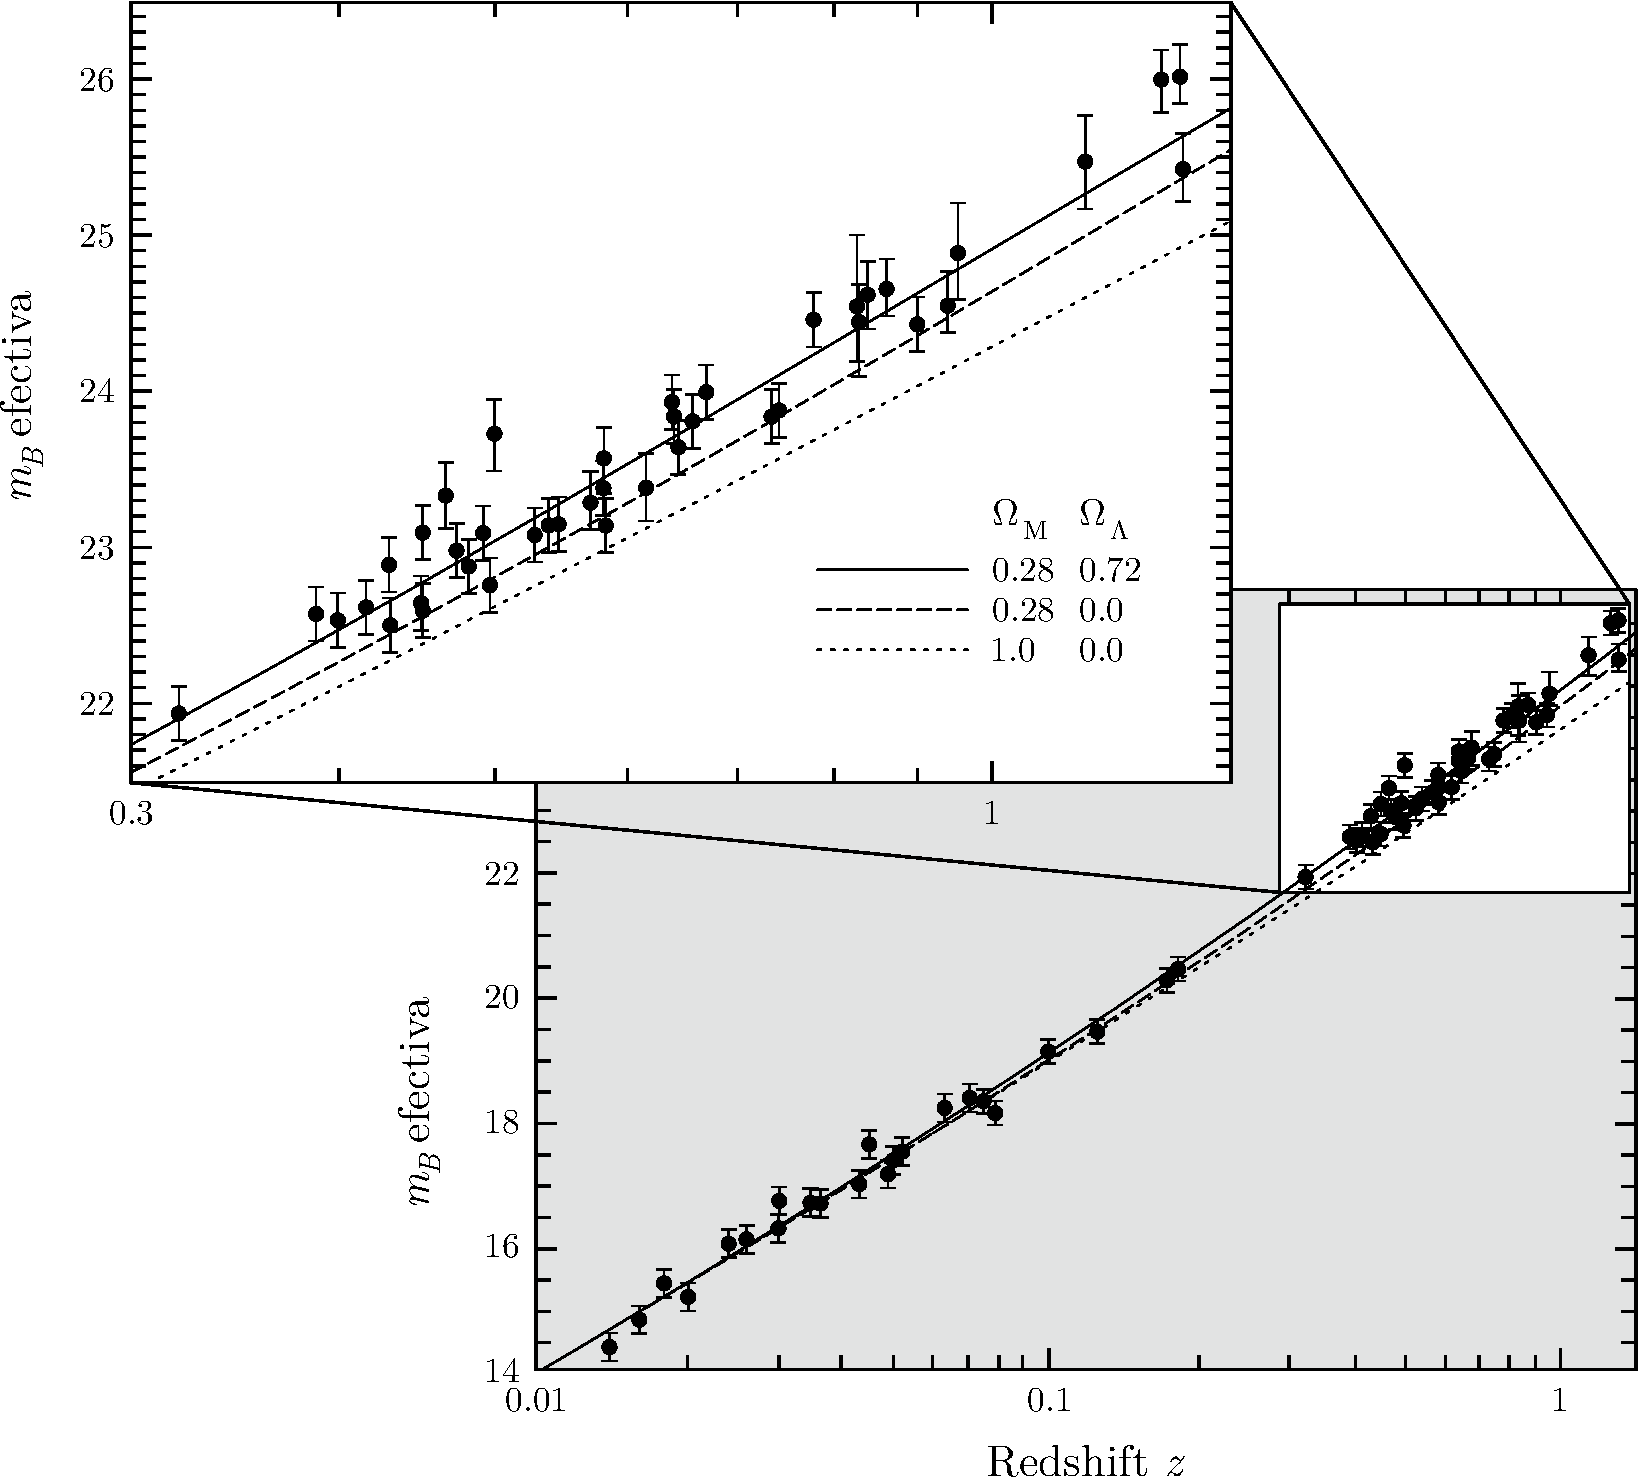
\includegraphics[width=0.9\textwidth]{./images/2-supernovae-redshift}
	\caption{Magnitud efectiva en el blau de supernoves en funció del \textit{redshift}}
	\label{fig:supernovae-redshift}
\end{figure}

És important, no obstant això, utilitzar galàxies del mateix tipus (podeu trobar la classificació dels tipus de galàxies a la \S~\ref{sec:galaxies}).

%-----------------------------------------------------------------
\subsection{Índex de color}
A la magnitud aparent, $m$, i l'absoluta, $M$, preses sobre totes les longituds d'ona de la llum emesa per una estrella se les anomena \textit{magnituds bolomètriques}, $m_{bol}$ i $M_{bol}$, respectivament.

Però, en realitat, la majoria de detectors mesuren el flux lluminós d'una estrella només dins d'algun interval $\Delta \lambda$ que depèn de la sensibilitat del detector.

El color d'una estrella pot determinar-se amb certa precisió mitjançant filtres que permeten el pas de la llum només en un rang donat de longituds d'ona.

En el sistema estàndard U, B, V, la magnitud aparent d'una estrella es mesura a través de tres filtres:
\begin{itemize}
	\item U: magnitud ultraviolada de l'estrella, es mesura amb un filtre centrat en $\SI{3650}{\angstrom}$ amb una amplada de $\SI{680}{\angstrom}$.
	\item B: magnitud blava de l'estrella, es mesura amb un filtre centrat en $\SI{4400}{\angstrom}$ amb una amplada de $\SI{980}{\angstrom}$.
	\item V: magnitud visual de l'estrella, es mesura amb un filtre centrat en $\SI{5500}{\angstrom}$ amb una amplada de $\SI{890}{\angstrom}$.
\end{itemize}

Si es coneix la distància $d$ a l'estrella un cop mesurades $U$, $B$, i $V$, mitjançant l'equació \eqref{eq:mMcolour} es poden determinar les magnituds absolutes de color $M_{U}$, $M_{B}$, i $M_{V}$:
\begin{align}\label{eq:mMcolour}
	m - M = 5 \log(\frac{d}{\SI{10}{\parsec}})
\end{align}

L'\textit{índex de color} $(U-B)$ d'una estrella és la diferència entre les seves magnituds ultraviolada i blava. De forma similar, l'índex de color $(B-V)$ d'una estrella és la diferència entre la magnitud blava i la visual, és a dir,
\begin{align}
\begin{aligned}
	U - B &= M_{U} - M_{B} \\
	B - V &= M_{B} - M_{V}
\end{aligned}
\end{align}
En vista de l'equació \eqref{eq:mMcolour}, l'índex de color no depèn de la distància a l'estrella.

Com que les magnituds decreixen amb la lluminositat, una estrella amb menor índex de color $(B-V)$ és \textit{més blava} que una amb major $(B-V)$.

Finalment, la magnitud bolomètrica, $m_{bol}$, d'una estrella i la seva magnitud visual estan relacionades mitjançant la seva correcció bolomètrica, $BC$, definida com
\begin{align}
	BC = m_{bol} - V = M_{bol} - M_{V}
\end{align}

%-----------------------------------------------------------------
%	LÍNIES ESPECTRALS
%	!TEX root = ./../main.tex
%-----------------------------------------------------------------
\section{Línies espectrals}
\subsection{Història}
\begin{itemize}
	\item  William Wollaston (1802) descobreix que la llum solar a través d'un prisma produeix un espectre tipus arc iris amb ratlles fosques superimposades (a l'espectre continu) a les longituds d'ona a les quals la llum solar havia estat absorbida (i.e., ratlles, o línies, d'absorció).
	\item  Joseph Fraunhofer (1814) va catalogar 475 d'aquestes ratlles d'absorció, les quals van resultar coincidir amb les produïdes per sals en una flama.
	\item Bunsen \& Kirchhoff van inventar l'espectroscopi. Aquest fa passar la llum d'una flama a través d'un prisma per ser analitzada. Kirchhoff va determinar 70 línies fosques en l'espectre solar corresponent a 70 línies brillants emeses (al laboratori) per vapor de ferro.

	Així doncs, els elements químics poden ser identificats sense ambigüitat per les seves línies espectrals, com si es tractessin d'empremtes dactilars.
\end{itemize}

%-----------------------------------------------------------------
\subsection{Lleis de Kirchhoff}
\begin{enumerate}[(i)]
	\item Un gas dens i calent (o un sòlid calent) produeix un espectre de radiació continu sense línies fosques.
	\item Un gas calent i difús produeix línies brillants (línies d'emissió).
	\item Si la llum d'una font d'espectre continu travessa un gas fres i difús, ratlles espectrals fosques (línies d'absorció) se superposen sobre l'espectre continu.
\end{enumerate}
D'aquesta manera es va poder identificar un gran nombre d'elements químics al Sol i a les estrelles, tot advertint-se que a diferents estrelles els correspon diferent espectre (ja que la composició química varia d'una estrella a una altra).
\begin{figure}[H]
	\centering
	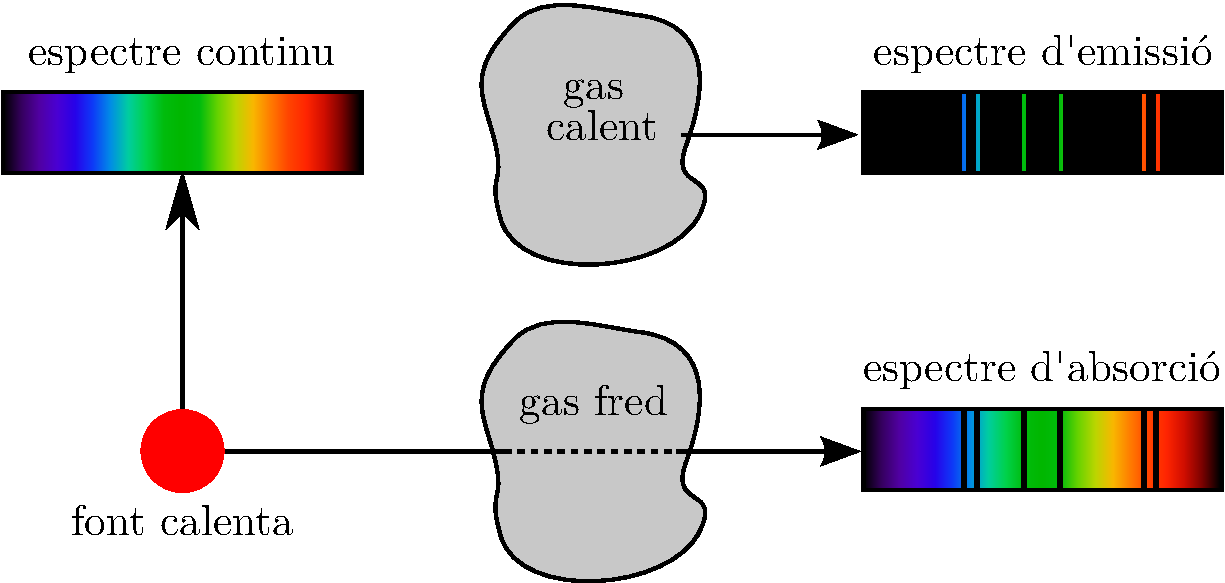
\includegraphics[width=0.75\textwidth]{./images/3-kirchhoff}
	\caption{Representació dels diferents espectres regits per les lleis de Kirchhoff}
	\label{fig:kirchhoff}
\end{figure}

\subsubsection*{Model de Bohr}
Les línies d'emissió són degudes al fotó emès en saltar un electró d'un nivell de major energia a un de menor energia. El procés oposat dóna lloc a línies d'absorció.
\begin{figure}[h]
	\centering
	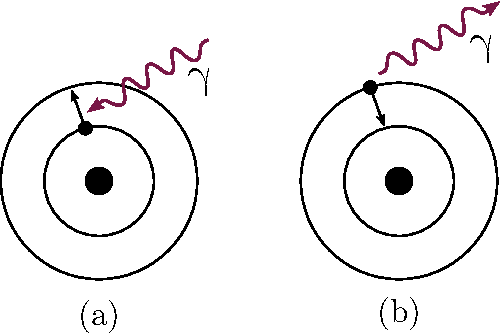
\includegraphics[width=0.4\textwidth]{./images/3-photon-abs-em}
	\caption{Absorció d'un fotó (a), i emissió d'un fotó (b)}
	\label{fig:photon-abs-em}
\end{figure}

En el model atòmic de Bohr
\begin{align}
	E_{n} = -\frac{13.6}{n^{2}} \si{\eV} \Rightarrow E_{\gamma} = E_{b} - E_{a} = 13.6 \qty(\frac{1}{n_{a}^{2}} - \frac{1}{n_{b}^{2}}) > 0
\end{align}
on $n$ és el nombre quàntic principal i $n_{a} < n_{b}$.
\begin{figure}[ht]
	\centering
	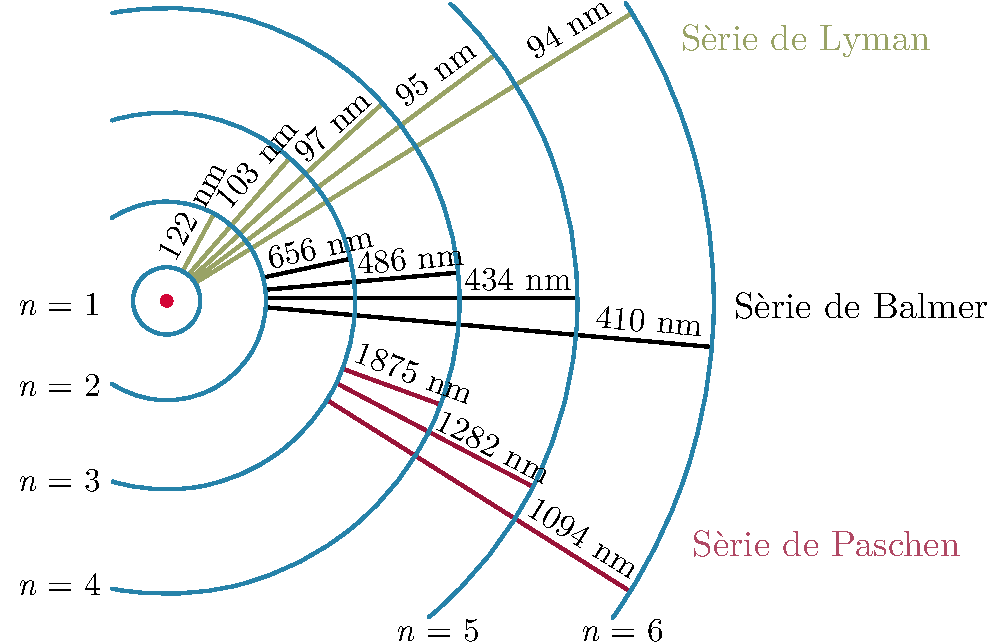
\includegraphics[width=0.7\textwidth]{./images/3-hydrogen-transitions}
	\caption{Transicions electròniques i les seves longituds d'ona resultants en l'emissió per a l'àtom d'hidrogen}
	\label{fig:hydrogen-transitions}
\end{figure}

\subsubsection*{Efecte Zeeman}
Divisió de les línies espectrals per la presència d'un camp magnètic d'intensitat $B$. En particular es compleix
\begin{align}
	\nu = \nu_{0} \pm \frac{eB}{4\pi \mu c}
\end{align}
on $e$ és la càrrega de l'electró, i $\mu$ és la massa reduïda.
\begin{figure}[h]
	\centering
	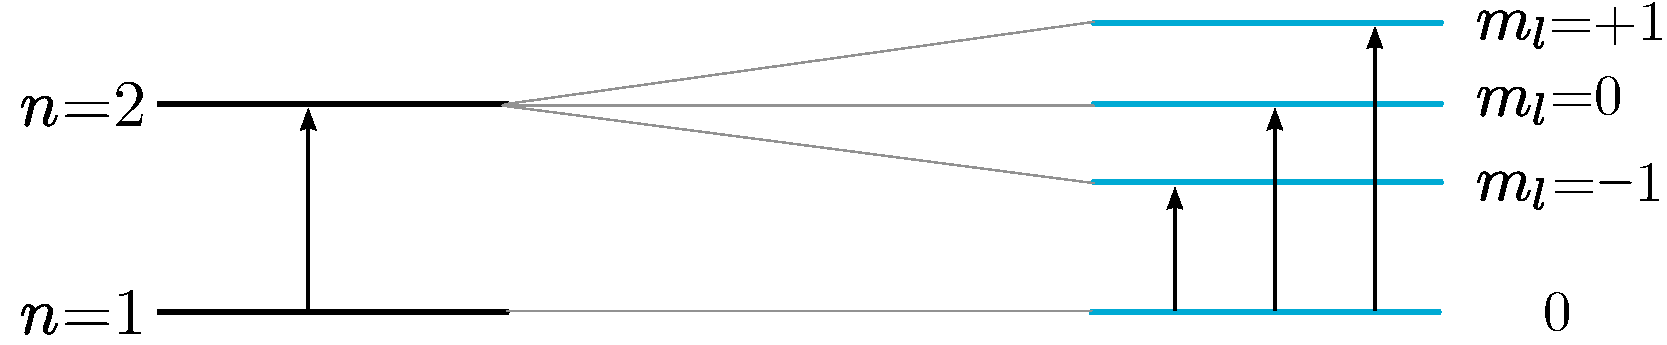
\includegraphics[width=0.7\textwidth]{./images/3-zeeman}
	\caption{Divisió de les línies d'absorció per efecte Zeeman}
	\label{fig:zeeman}
\end{figure}

La divisió de les línies espectrals indica la presència de camps magnètics, tal com passa a les taques solars.

%-----------------------------------------------------------------
\subsection{Seqüència dels espectres estel·lars de Harvard}
% FIXME: cannon@sec:bio
La catalogació que Annie Jump Cannon (1863), astrònoma americana, va fer de les estrelles ha estat fonamental per l'actual classificació estel·lar. La classificació espectral de Harvard va en sentit decreixent de temperatures: O B A F G K M R N S. Cada lletra, alhora, se subdivideix en deu (e.g., A0-A9).

Per facilitat, s'acostuma a fer servir la següent regla mnemotècnica per recordar els tipus d'espectres estel·lars:
\begin{quote}
	\textit{‘Oh! Be A Fine Girl, Kiss Me Right Now, Sweetheart!’}
\end{quote}

A continuació podeu consultar una taula que resumeix la classificació espectral estel·lar de Harvard.
\begin{table}[H]
	\centering
		\begin{tabular}{ccccc}
		\toprule
		Tipus & $M$ ($\times \si{\Msun}$) & $R$ ($\times \si{\Rsun}$) & $L$ ($\times \si{\Lsun}$) & $T$ ($\times \SI{e3}{\K}$) \\
		\midrule
		O & \numrange{20}{100} & $\sim\num{15}$ & \numrange{e5}{e6} & \numrange{30}{50} \\
		B & \numrange{3}{18} & $\sim\num{7}$ & \numrange{100}{52000} & \numrange{10.5}{30} \\
		A & \numrange{1.5}{3} & $\sim\num{2.5}$ & \numrange{7}{50} & \numrange{7.2}{9.5} \\
		F & \numrange{1.2}{1.6} & $\sim\num{1.3}$ & \numrange{2}{6.5} & \numrange{6.1}{7.2} \\
		G & \numrange{0.8}{1.1} & $\sim\num{1.1}$ & \numrange{0.4}{2} & \numrange{5.3}{6} \\
		K & \numrange{0.5}{0.8} & $\sim\num{0.9}$ & \numrange{0.1}{0.4} & \numrange{3.9}{5.2} \\
		M & $< \num{0.5}$ & $\sim\num{0.4}$ & $<\num{0.08}$ & $<\num{3.9}$ \\
		\bottomrule
		\end{tabular}
	\caption{Comparació de les característiques físiques de les estrelles de la seqüència principal}
	\label{tab:harvard}
\end{table}

\begin{figure}[h]
	\centering
	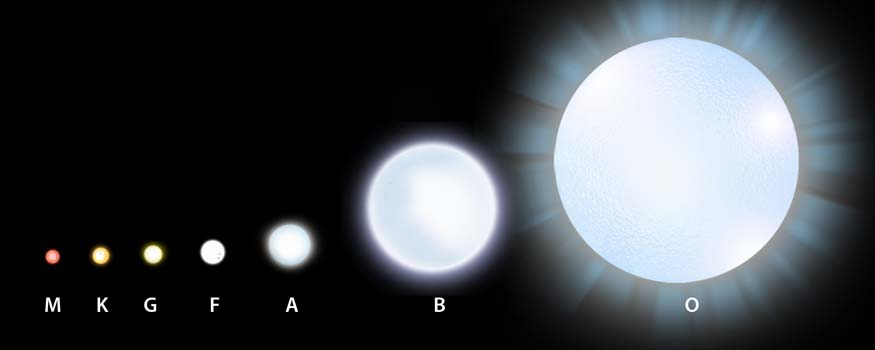
\includegraphics[width=0.8\textwidth]{./images/3-harvard-classification}
	\caption{Comparació visual dels diferents tipus d'espectres estel·lars de la classificació de Harvard}
	\label{fig:harvard-classification}
\end{figure}

%-------------------------------
\subsubsection*{Estrelles tipus O}
Les més brillants, calents i massives de la seqüència principal. De color blau, emeten la major part de la seva energia en l'ultraviolat.

Posseeixen una temperatura efectiva entre $\SI{30 e3}{\K}$ i valors superiors a $\SI{50 e3}{\K}$ i una lluminositat entre $\SI{e5}{\Lsun}$ i valors més enllà de $\SI{e6}{\Lsun}$. Les seves masses varien entre $\SI{20}{\Msun}$ i $\SI{100}{\Msun}$. Cremen combustible nuclear a un ritme molt elevat, de forma que només \textit{viuen} de 3 a 6 milions d'anys.

Com a conseqüència de la seva alta temperatura, les línies de l'hidrogen dels seus espectres són febles. Les línies que dominen són les de He II.

Són escasses, només es coneixen un grapat del tipus O3 i O4 (no es coneix cap estrella de O0 a O2).

Les més brillants a simple vista són Delta Orionis i Zeta Orionis (ambdues O9 supergegants).

%-------------------------------
\subsubsection*{Estrelles tipus B}
Els seus espectres són dominats per les línies d'absorció de l'hidrogen i de l'heli neutre. Són de color blau i calents. Emeten principalment en l'ultraviolat.

En la seqüència principal les seves temperatures se situen en l'interval de $\SI{10500}{\K}$ a $\SI{30000}{\K}$, amb lluminositats de $\SI{100}{\Lsun}$ a $\SI{52000}{\Lsun}$ i masses de $\SI{3}{\Msun}$ a $\SI{18}{\Msun}$.

Les supergegants posseeixen masses de fins a $\SI{25}{\Msun}$ i lluminositats de fins a $\SI{260 e3}{\Lsun}$. Rigel és una supergegant, mentre que Spica [\href{http://apod.nasa.gov/apod/ap021214.html}{APOD~021204}] i Regulus són estrelles nanes.

Viuen només unes desenes de milions d'anys.

%-------------------------------
\subsubsection*{Estrelles tipus A}
Els seus espectres són dominats per les línies d'absorció de l'hidrogen. En aquests espectres es donen les línies d'absorció més intenses en estrelles de la seqüència principal. Són de color blau-blanquinós.

Les de la seqüència principal posseeixen temperatures en el rang de $\SI{7200}{\K}$ a $\SI{9500}{\K}$ i són entre 7 i 50 vegades més lluminoses que el Sol, amb masses entre 1.5 i 3 masses solars.

Les supergegants (com Deneb [\href{http://apod.nasa.gov/apod/ap961212.html}{APOD~961212}]) són més massives (fins a $\SI{16}{\Msun}$), amb temperatures de fins a $\SI{9700}{\K}$ i lluminositats per sobre de $\SI{35000}{\Lsun}$.

Sírius és de tipus espectral A1 i Vega és del tipus A0.

%-------------------------------
\subsubsection*{Estrelles tipus F}
Les línies d'absorció de l'hidrogen decauen fortament en intensitat del tipus F0 al F9 al temps que les línies del calci augmenten en intensitat i moltes altres línies corresponents a metalls comencen a fer-se visibles.

Les de la seqüència principal posseeixen temperatures entre $\SI{6100}{\K}$ i $\SI{7200}{\K}$, mentre que les supergegants són uns pocs centenars de kelvin més fredes.

Les masses en la seqüència principal se situen entre $\SI{1.2}{\Msun}$ i $\SI{1.6}{\Msun}$; les lluminositats, entre $\SI{2}{\Lsun}$ i $\SI{6.5}{\Lsun}$. Les supergegants tenen fins a 12 vegades la massa del Sol i lluminositats de fins a $\SI{32000}{\Lsun}$.

Les estrelles Polaris [\href{http://apod.nasa.gov/apod/ap991006.html}{APOD~991006}] i Procyon són de tipus F.

%-------------------------------
\subsubsection*{Estrelles tipus G}
Les pertanyents a la seqüència principal tenen temperatures efectives entre $\SI{5300}{\K}$ i $\SI{6000}{\K}$, per això són de color groc. Les gegants són entre 100 i 500 kelvin més fredes i les supergegants posseeixen temperatures entre $\SI{4500}{\K}$ i $\SI{5500}{\K}$.

L'espectre del Sol (tipus G2) és dominat per línies de l'ió \ch{Ca+} i de metalls neutres. En estrelles de tipus G més fredes comencen a advertir-se les bandes de \ch{CH} i \ch{CN}.

Les masses en la seqüència principal i de les gegants varien entre $\SI{0.8}{\Msun}$ i $\SI{1.1}{\Msun}$; la massa de les supergegants varia entre $\SI{10}{\Msun}$ i $\SI{12}{\Msun}$.

Les lluminositats de les gegants varia entre $\SI{30}{\Lsun}$ i $\SI{60}{\Lsun}$; les lluminositats de les supergegants, entre $\SI{10000}{\Lsun}$ i $\SI{300000}{\Lsun}$.

L'estrella Capella\footnote{[\href{http://apod.nasa.gov/apod/ap021106.html}{APOD~021106}]: l'Hexàgon Hivernal és format per Aldebaran, Capella, Castor, Procyon, Rigel, i Sírius.} és una gegant de tipus G.

%-------------------------------
\subsubsection*{Estrelles tipus K}
En la seqüència principal tenen temperatures entre $\SI{3900}{\K}$ i $\SI{5200}{\K}$, les gegants són entre 100 i 400 kelvin més fredes i les supergegants són uns quants centenars de kelvin més fredes encara. Són de color taronja.

Les masses en la seqüència principal van entre $\SI{0.5}{\Msun}$ i $\SI{0.8}{\Msun}$; les seves lluminositats, entre $0\SI{0.1}{\Lsun}$ i $\SI{0.4}{\Lsun}$. Les gegants posseeixen masses entre $\SI{1.1}{\Msun}$ i $\SI{1.2}{\Msun}$ i lluminositats entre $\SI{60}{\Lsun}$ i $\SI{300}{\Lsun}$. Les supergegants, com a màxim, arriben a $\SI{13}{\Msun}$ i $\SI{40000}{\Lsun}$.

Els seus espectres es caracteritzen per línies d'absorció del ferro i titani neutres, i calci neutre i \ch{Ca+} (aquestes dues últimes són línies intenses). La intensitat de les bandes de \ch{CN} i \ch{TiO} es reforcen notablement des de K0 fins a K9.

Arcturus [\href{http://apod.nasa.gov/apod/ap020910.html}{APOD~020910}] és una gegant K1 i Aldebaran és una gegant K5.

%-------------------------------
\subsubsection*{Estrelles tipus M}
Són estrelles de molt baixa temperatura efectiva (inferior a $\SI{3900}{\K}$) de color vermellós. Emeten la major part de la seva radiació en l'infraroig.

Les nanes tipus M (conegudes com \textit{nanes rojes}) se situen al tram inferior de la seqüència principal. Com que posseeixen lluminositats de $\SI{0.08}{\Lsun}$ com a màxim, ni tan sols les més properes a nosaltres (e.g., Proxima Centauri) poden ser vistes sense telescopi. Les seves masses, en la seqüència principal, no arriben a $\SI{0.5}{\Msun}$.

La seva vida mitjana podria ser major que l'edat actual de l'Univers.

Moltes estrelles tipus M són gegants amb masses entre $\SI{1.2}{\Msun}$ i $\SI{1.3}{\Msun}$ i amb lluminositats en torn a $\SI{300}{\Lsun}$.

Les supergegants, com Betelgeuse i Antares, posseeixen masses entre $\SI{13}{\Msun}$ i $\SI{25}{\Msun}$ i lluminositats entre $\SI{40000}{\Lsun}$ i $\SI{500000}{\Lsun}$. La seva mida pot ser tan gran com l'òrbita de Júpiter.

Els seus espectres solen ser dominats per amples bandes d'absorció moleculars, com el \ch{TiO}, però també són presents línies d'absorció de metalls neutres.

%-------------------------------
\subsubsection*{Estrelles tipus R \& N (\textsl{carbon stars})}
Gegants roges i fredes en avançat estat d'evolució. Els seus espectres són dominats per fortes bandes corresponents a les molècules \ch{CN}, \ch{CH}, i \ch{C2} (per això el nom de \textit{carbon stars}).

La presència de \ch{Li} indica que aquests elements (\ch{C}, \ch{Li}, \ch{N}) han estat produïts al nucli de l'estrella mitjançant reaccions nuclears i transportats per convecció a la superfície.

Ja que el carbó només es pot produir pel procés triple--$\alpha$ a molt alta temperatura, aquestes estrelles es troben en un estat evolutiu força avançat.

Les estrelles tipus R posseeixen temperatura efectiva entre $\SI{4000}{\K}$ i $\SI{5000}{\K}$; les tipus N, aproximadament $\SI{3000}{\K}$.

Les tipus R poden ser fins a 10 vegades més lluminoses que les tipus N.

%-------------------------------
\subsubsection*{Estrelles tipus S}
Gegants roges d'espectre similar a les del tipus $M$, excepte que la banda dominant no és \ch{TiO} sinó el \ch{ZrO}; també es troben òxids de lantà, itri, i bari. Aquests elements deuen haver estat creats al nucli de l'estrella en les seves últimes etapes evolutives.

La majoria de les estrelles de tipus S posseeixen lluminositat irregular o bé de llarg període.

%-----------------------------------------------------------------
\subsection{Relació de l'espectre amb la temperatura}
Les velocitats de les partícules d'un gas segueixen una distribució de Maxwell-Boltzmann:
\begin{align}
	n_{v} \dd{v} = n \qty(\frac{m}{2\pi k_{B} T}) \exp[-\frac{mv^{2}}{2k_{B}T}] 4\pi v^{2} \dd{v}
\end{align}
on $n_{v} \dd{v}$ és la densitat numèrica de partícules amb velocitat en l'interval $[v, v + \dd{v}]$.
També definim \textit{most probable speed}, $v_{mp}$, i \textit{root mean square speed}, $v_{rms}$:
\begin{align}
	v_{mp} = \sqrt{\frac{2k_{B}T}{m}}, \quad v_{rms} = \sqrt{\frac{3k_{B}T}{m}}
\end{align}
\begin{figure}[h]
	\centering
	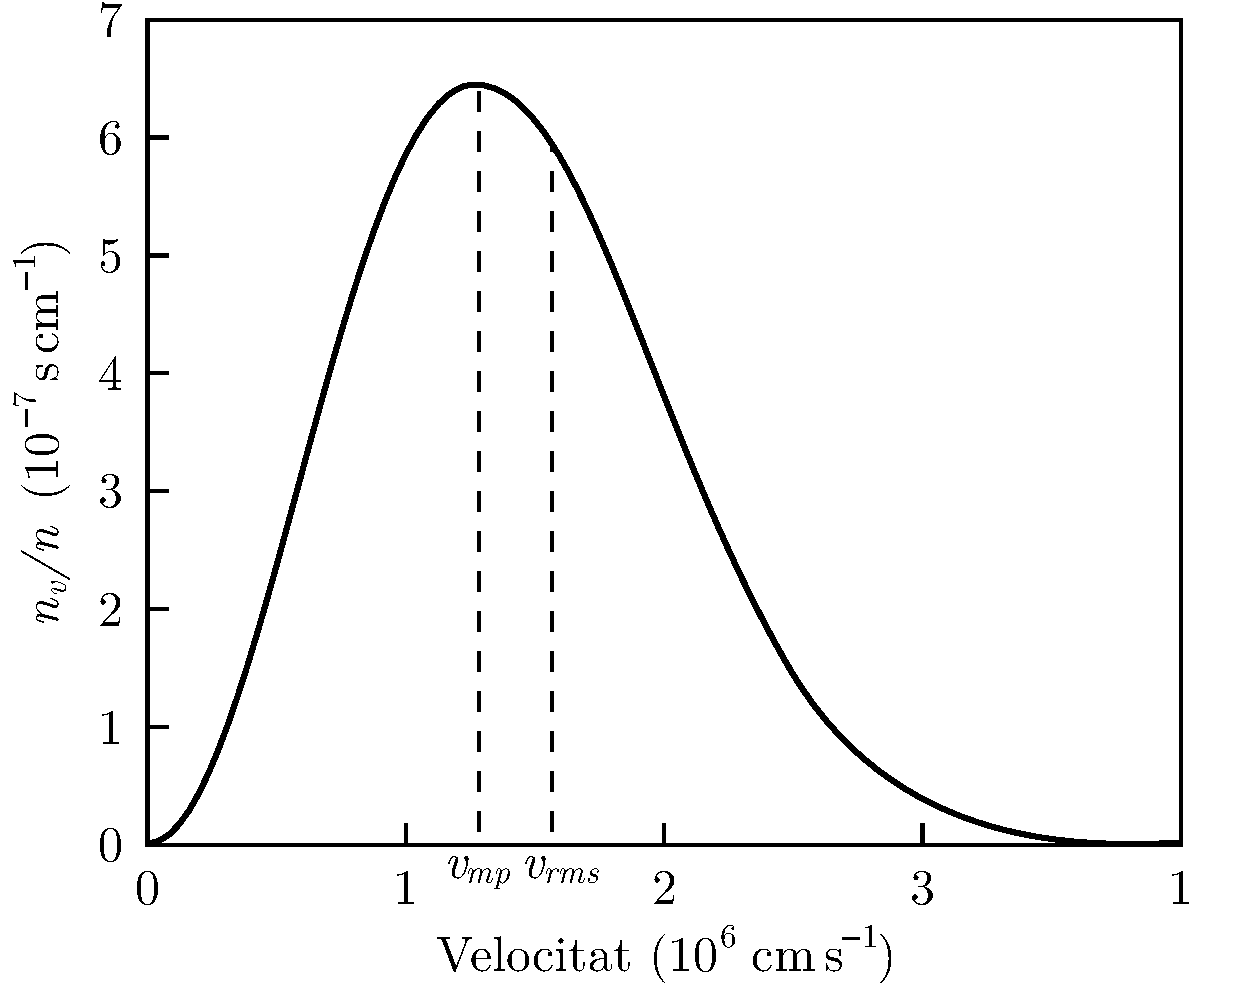
\includegraphics[width=0.65\textwidth]{./images/3-maxwell-boltzmann}
	\caption{Distribució de Maxwell--Boltzmann per a àtoms d'hidrogen a $T = \SI{10000}{\K}$, on $v_{mp} = \SI{1.29 e6}{\cm\per\s}$ i $v_{rms} = \SI{1.57 e6}{\cm\per\s}$}
	\label{fig:maxwell-boltzmann}
\end{figure}

La cua de la distribució cau aproximadament com $\exp[-\dfrac{mv^{2}}{2k_{B}T}]$.

La mecànica estadística ens diu que el quocient entre el nombre d'àtoms en dos estats idèntics $a$ i $b$ accessibles al sistema (el qual es troba en equilibri termodinàmic) és
\begin{align}
	\frac{N_{a}}{N_{b}} = \frac{g_{b}}{g_{a}} \exp[- \frac{E_{b} - E_{a}}{k_{B} T}]
\end{align}
on $g_{a}$ i $g_{b}$ són el nombre d'estats amb energies $E_{a}$ i $E_{b}$, respectivament, és a dir, la degeneració. Per a l'àtom d'hidrogen $g_{H,n} = 2n^{2}$.
\begin{example}
	Sigui un gas d'àtoms neutres d'hidrogen. A quina temperatura hi haurà igual nombre d'àtoms en l'estat fonamental que el primer estat excitat?
	\begin{align*}
		\frac{N(n=1)}{N(n=2)} = \frac{2\times 2^{2}}{2\times 1^{2}} \exp[\frac{13.6}{k_{B}T} \qty(\frac{1}{2^{2}} - \frac{1}{1^{2}})] \equiv 1 \Rightarrow T = \SI{8.54 e4}{\K}
	\end{align*}
\end{example}

Igualment, el nombre relatiu d'àtoms en diferents estats d'ionització ve determinat (en l'equilibri) per la temperatura segons l'equació de Saha~\eqref{eq:saha}.
\begin{figure}[h]
	\centering
	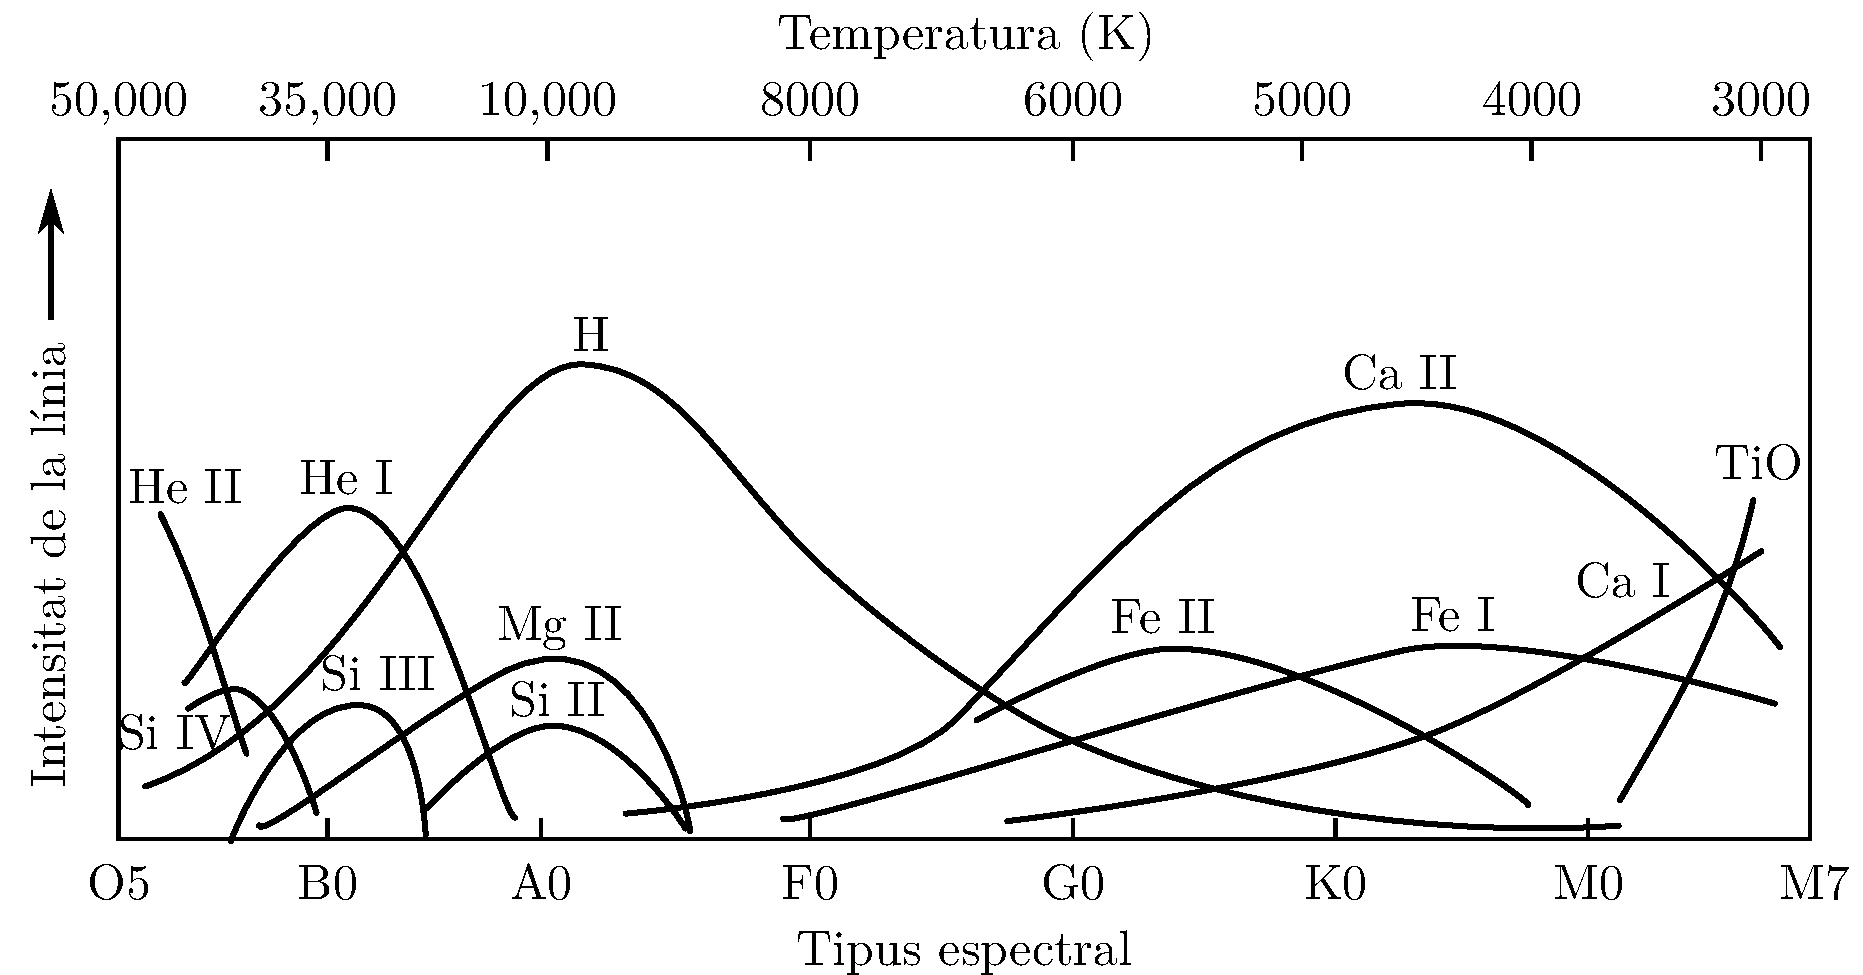
\includegraphics[width=0.95\textwidth]{./images/3-spectral-strenght}
	\caption{Dependència de les intensitats de les línies espectrals amb la temperatura}
	\label{fig:spectral-strenght}
\end{figure}

Per exemple, en l'equació de recombinació--ionització $e^{-} + p \leftrightarrows \ch{H} + \gamma$, la condició d'equilibri tèrmic és
\begin{align*}
	\mu(e^{-}) + \mu(p) = \mu(\ch{H}), \quad \qty[\mu(\gamma) \equiv 0]
\end{align*}
Aquesta condició condueix a
\begin{align}\label{eq:saha}
	\frac{x^{2}}{x-1} = \frac{1}{n} \qty[\frac{2\pi m_{e} k_{B} T}{h^{2}}] e^{-B/K_{B}T}
\end{align}
on $B = \SI{13.6}{\eV}$ és l'energia d'ionització, $x= n_{e}/n_{p}$, i $n = n_{p} + n_{H}$.
% \begin{sproof}
%     TODO: proof (class)
%     \url{https://en.wikipedia.org/wiki/Saha_ionization_equation}
% \end{sproof}

Llavors, el conjunt de línies espectrals d'una estrella ens proporciona informació no només de l'abundància relativa d'elements químics en les capes més externes, sinó també sobre el tipus espectral (O, B, A, etc.), estats d'ionització, i pressió (ja que a l'equació de Saha $n_{e}$ pot substituir-se per $p_{e} = n_{e} K_{B}T$).

%-----------------------------------------------------------------
\subsection{Efecte Doppler}
En general els espectres estel·lars es veuen desplaçats respecte els seus corresponents al laboratori. Això és degut a l'efecte Doppler.
\begin{figure}[h]
	\centering
	
\includegraphics[width=0.7\textwidth]{./images/3-doppler}
	\caption{Quan la font de llum s'allunya de l'obsrvador, es produeix un \textit{redshift}, mentre que si la font s'hi apropa, es produeix un \textit{blueshift}}
	\label{fig:doppler}
\end{figure}

Si la velocitat radial (velocitat al llarg de la visual), $v_{r}$, de l'estrella és baixa ($v_{r} \ll c$), tenim
\begin{align}
	\frac{\Delta \lambda}{\lambda} = \frac{\lambda_{obs} - \lambda_{em}}{\lambda_{em}} = \frac{v_{r}}{c}
\end{align}
la qual cosa permet determinar $v_{r}$ amb una aproximació de $\SI{\pm10}{\m\per\s}$.

Per determinar $v_{\theta}$ (perpendicular a $v_{r}$) és necessari conèixer la distància a l'estrella, sigui aquesta $d$, i el seu desplaçament angular per unitat de temps, $\mu$, (típicament en $\si{\arcsecond\per\year}$), la qual cosa s'aconsegueix a través de l'observació durant un període de temps suficientment llarg. Es veu fàcilment que
\begin{align}
	v_{\theta} = \mu d
\end{align}

La velocitat de l'estrella respecte al Sol serà, doncs
\begin{align}
	v = \sqrt{v_{r}^{2} + v_{\theta}^{2}}
\end{align}
La velocitat mitjana del conjunt d'estrelles més pròximes al Sol és d'uns $\SI{25}{\km\per\s}$.

En realitat, la determinació de $v_{r}$ no és molt simple, ja que s'ha de tenir en compte la velocitat ($\approx$ constant) de la Terra en la seva òrbita solar ($\SI{29.8}{\km\per\s}$). Això dóna lloc a que $\lambda_{obs}$ variï sinusoïdalment al llarg de l'any. No obstant això, només cal restar (o sumar) la component de la velocitat terrestre al llarg de la visual per obtenir la vertadera velocitat radial de l'estrella respecte al Sol.

%-----------------------------------------------------------------
\subsection{Espectrògraf}
S'utilitza per determinar l'espectre d'estrelles i galàxies. Es fa passar la llum estel·ar per una escletxa, es col·lima mitjançant un mirall i es dirigeix sobre una xarxa de difracció. L'espectre resultant de la xarxa s'enfoca sobre una placa fotogràfica o sobre un detector electrònic.

La xarxa de difracció (una llarga sèries de doble escletxes molt pròximes entre elles) dóna lloc a màxims i mínims de difracció. Sigui $a$ la separació entre dues escletxes adjacents, llavors, es compleix
\begin{align}
	a \sin \theta = n \lambda, \quad n \in \mbb{N}
\end{align}
on $\theta$ és l'angle de difracció i $n$ és l'ordre de l'espectre.
\begin{figure}[H]
	\centering
	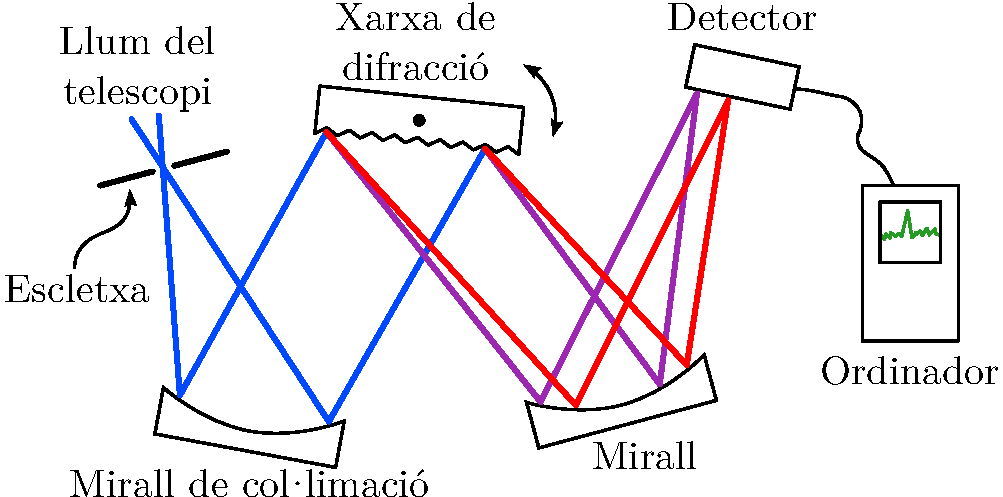
\includegraphics[width=0.65\textwidth]{./images/3-spectrograph}
	\caption{Diagrama d'un espectrògraf}
	\label{fig:spectrograph}
\end{figure}

La capacitat de resoldre dues longituds d'ona molt pròximes, separades per $\Delta \lambda$, depèn de l'ordre $n$ de l'espectre i del nombre total $N$ d'escletxes il·luminades.

La màxima resolució a la qual l'espectrògraf pot arribar és
\begin{align}
	\Delta \lambda = \frac{\lambda}{nN}
\end{align}
El quocient $\Delta \lambda / \lambda$ ens dóna el poder de resolució de la xarxa de difracció (a menor quocient, major poder).

%-----------------------------------------------------------------
\subsection{Diagrames de Hertzsprung--Russell}\label{sec:hertz-russell}
Si s'accepta que la superfície d'una estrella es comporta, aproximadament, com un cos negre, tindrem una relació entre la seva lluminositat $L$, el seu radi $R$, i la seva temperatura efectiva $T_{e}$:
\begin{align}\label{eq:hertz-russell}
	L = 4 \pi R^{2} \sigma T_{e}^{4}
\end{align}
on $\sigma$ és la constant d'Stefan--Boltzmann.

Aquesta relació és consistent amb el diagrama proposat per Hertzsprung (1905) i, independentment, per Russell (1912).

El radi d'una estrella pot calcular-se a partir de l'equació \eqref{eq:hertz-russell} i la seva posició al diagrama de Hertzsprung--Russell.

És important destacar les següents franges dels diagrames de Hertzsprung--Russell:
\begin{itemize}
	\item Una franja aproximadament diagonal (en què es troba el Sol) amb $\SI{0.1}{\Rsun} \leq R \leq \SI{20}{\Rsun}$. Aquesta franja s'anomena \textit{seqüència principal}.
	\item Una franja d'estrelles gegants (a dalt de la zona inferior de la seqüència principal) amb $\SI{10}{\Rsun} \leq R \leq \SI{100}{\Rsun}$.
	\item Una altra franja, menys poblada, de supergegants amb radis $\sim \SI{e3}{\Rsun}$.
\end{itemize}
\begin{figure}[h]
	\centering
	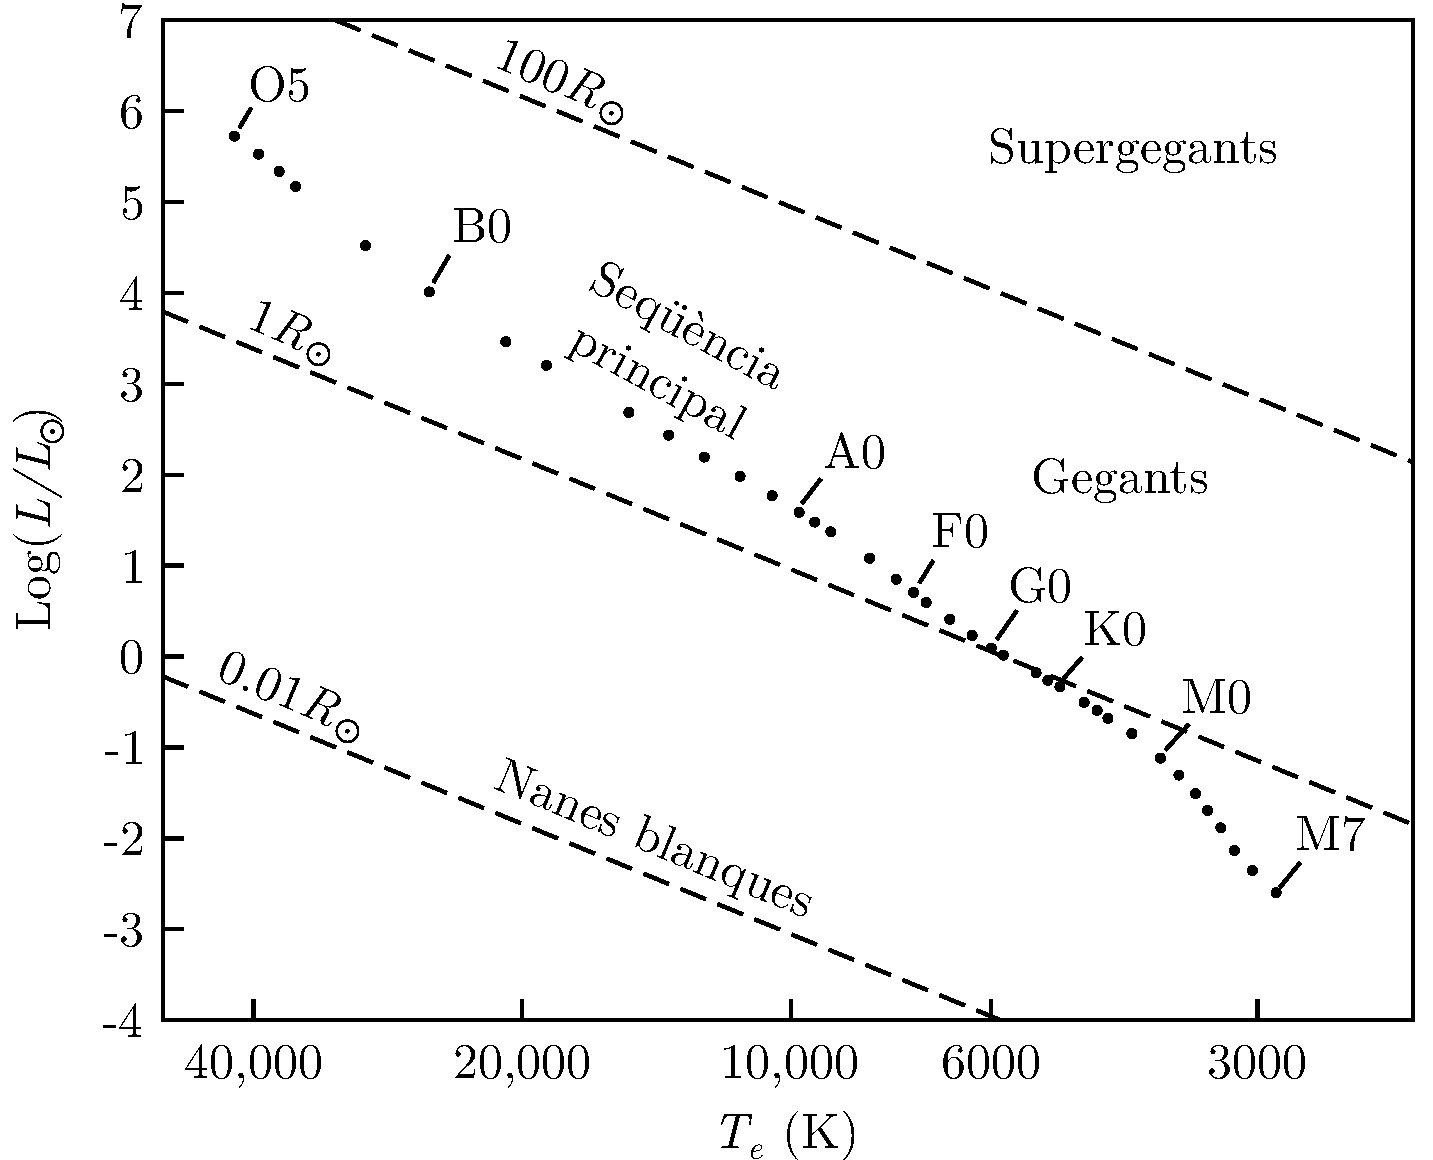
\includegraphics[width=0.75\textwidth]{./images/3-hertzsprung-russell}
	\caption{Diagrama de Hertzsprung--Russell teòric. Les línies discontínues indiquen les estrelles de radi constant.}
	\label{fig:hertzsprung-russell}
\end{figure}

El rang de lluminositats estel·lars és aproximadament de
\begin{align*}
	\SI{5 e-4}{\Lsun} \lesssim L \lesssim \SI{e6}{\Lsun}
\end{align*}
Sobre la seqüència principal es dóna la relació lluminositat--massa
\begin{align}
	\frac{L}{\Lsun} \propto \qty(\frac{M}{\Msun})^{\nu}, \quad \text{on } \nu = \begin{cases} 1 & \text{estrelles molt massives} \\ 3 & \text{estrelles massives} \\ 5.5 & \text{estrelles poc massives} \end{cases}
\end{align}
La densitat en les estrelles de la seqüència principal és $\sim \SI{1}{\g\per\cubic\cm}$.
\begin{itemize}
	\item El Sol és una estrella de la seqüència principal de tipus espectral G2. $\Msun = \SI{1.988 e 33}{\g}$, $\Rsun = \SI{6.955 e10}{\cm} \Rightarrow \rho_{\odot} = \SI{1.411}{\g\per\cubic\cm}$.
	\item Sírius, l'estrella més brillant del firmament nocturn, és del tipus espectral A1. $M_{S} = \SI{2.3}{\Msun}$, $R_{S} = \SI{1.6}{\Rsun} \Rightarrow \rho_{S} = \SI{0.792}{\g\per\cubic\cm}$.
\end{itemize}
En canvi, les gegants i supergegants són molt menys denses.
\begin{itemize}
	\item Betelgeuse ($M_{B} \approx \SI{12}{\Msun}$) és una estrella polsant de radi màxim de $\SI{e3}{\Rsun}$. Llavors, té una densitat de $\rho_{B} \sim \SI{e-8}{\g\per\cubic\cm}$, menys densa, doncs, que l'aire a nivell del mar.
\end{itemize}

\begin{example}
	La temperatura efectiva d'una estrella és $T_{e} = \SI{12000}{\K}$ i la seva magnitud absoluta és $M = 0.0$. Trobeu el seu radi sabent que la temperatura efectiva del Sol és $T_{e,\odot} = \SI{5800}{\K}$ i la seva magnitud absoluta és $\Msun = 4.76$.

	Recordem que si dues estrelles es troben a la mateixa distància de la Terra, la relació entre les seves magnituds absolutes és $M_{1} - M_{2} = - 2.5 \log (L_{1}/L_{2})$, i si una de les estrelles és el Sol, llavors
	\begin{align*}
		M - \Msun = - 2.5 \log(\frac{L}{\Lsun})
	\end{align*}
	Tenint en compte que $L = 4 \pi R^{2} \sigma T_{e}^{4}$, s'arriba a
	\begin{align*}
		M - \Msun = - 2.5 \qty[ 2\log(\frac{R}{\Rsun}) + 4\log( \frac{T_{e}}{T_{e,\odot}} ) ]
	\end{align*}
	és a dir
	\begin{align*}
	\begin{aligned}
		-\qty(\frac{M-\Msun}{5}) &= \log \qty[\qty(\frac{R}{\Rsun}) \qty(\frac{T_{e}}{T_{e,\odot}})^{2}]\\
		\Rightarrow \frac{R}{\Rsun} &= \qty(\frac{T_{e,\odot}}{T_{e}})^{2} 10^{-(M-\Msun)/5} \approx 2
	\end{aligned}
	\end{align*}
	Llavors $R \approx \SI{2}{\Rsun} = \SI{1.391 e6}{\km}$.
\end{example}

%-----------------------------------------------------------------
%	CAMP DE RADIACIÓ
%	!TEX root = ./../main.tex
%-----------------------------------------------------------------
\section{Camp de radiació}
\subsection{Conceptes bàsics}
La llum que rebem d'una estrella procedeix de la seva atmosfera, és a dir, de les capes superiors i transparents de gas que envolten l'interior (opac) de l'estrella. Aquí descriurem breument com viatja la llum a través de aquest gas.
\begin{figure}[h]
	\centering
	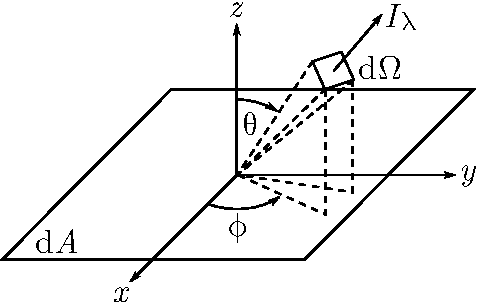
\includegraphics[width=0.4\textwidth]{./images/4-intensitat}
	\caption{Intensitat $I_{\lambda}$}
	\label{fig:intensitat}
\end{figure}

La figura \ref{fig:intensitat} mostra un raig de llum amb longitud d'ona entre $\lambda$ i $\lambda + \dd{\lambda}$ travesant una superfície $\dd{A}$ sota un angle $\theta$ respecte a la normal en un con d'angle sòlid $\dd{\Omega}$.

\subsubsection*{Intensitat}
\begin{defi}[Intensitat mitjana]
	Sigui $E_{\lambda}\dd{\lambda}$ l'energia que el raig porta a aquell con en un temps $\dd{t}$. Es defineix la intensitat mitjana d'aquest rang al quocient
	\begin{align}
	\bar{I}_{\lambda} = \frac{E_{\lambda} \dd{\lambda}}{\dd{\lambda} \dd{t} \dd{A} \cos \theta \dd{\Omega}}
	\end{align}
	Al CGS té unitats de $\qty[\bar{I}_{\lambda}] = \si{\erg \per \s \per \square\cm \per \steradian}$.
\end{defi}

\begin{defi}[Intensitat específica]
	En el límit $\dd{\Omega} \to 0$ el raig no es dispersa i la corresponent intensitat $I_{\lambda}$ es coneix com intensitat específica o simplement intensitat.
\end{defi}
En general la intensitat depèn de la direcció, de forma que la intensitat mitjana (sobre la direcció) s'escriu
\begin{align}
	\ev{I_{\lambda}} = \frac{1}{4\pi} \int I_{\lambda} \dd{\Omega} = \frac{1}{4\pi} \int_{\phi = 0}^{2\pi} \int_{\theta = 0}^{\pi} I_{\lambda} I_{\lambda} \sin \theta \dd{\theta} \dd{\phi}
\end{align}
Per a un camp isòtrop, $\ev{I_{\lambda}} \equiv I_{\lambda}$.

\subsubsection*{Energia}
\begin{defi}[Densitat d'energia]
	En un volum qualsevol (però que contingui moltes longituds d'ona), la densitat d'energia en l'interval $(\lambda, \lambda + \dd{\lambda})$ és
	\begin{align}
		u_{\lambda} \dd{\lambda} = \frac{1}{c} \int I_{\lambda} \dd{\lambda} \dd{\Omega} = \frac{4\pi}{c} \ev{I_{\lambda}} \dd{\lambda}
	\end{align}
\end{defi}
Per a un camp de radiació de cos negre (que és isòtrop), tenim que
\begin{align*}
	u_{\lambda} \dd{\lambda} = \frac{4\pi}{c} B_{\lambda} \dd{\lambda} = \frac{8\pi h c}{\lambda^{5}(e^{hc/\lambda k_{B} T} - 1)} \dd{\lambda}
\end{align*}
i en termes de la freqüència ($\nu = c/\lambda$), es pot reescriure com
\begin{align*}
	u_{\lambda} \dd{\nu} = \frac{4\pi}{c} B_{\nu} \dd{\nu} = \frac{8\pi h \nu}{\nu^{3}(e^{h \nu/k_{B} T} - 1)} \dd{\nu}
\end{align*}
Sumant totes les longituds d'ona, la densitat d'energia radiant d'un cos negre és
\begin{align}
	U = \int_{0}^{\infty} u_{\lambda} \dd{\lambda} = \frac{4\pi}{c} \int_{0}^{\infty} B_{\lambda}(T) \dd{\lambda} = \frac{4 \sigma}{c} T^{4} \equiv a T^{4}
\end{align}
on $a \equiv \dfrac{4\sigma}{c} = \SI{7.566}{\erg \per \cubic\cm \per \quartic\K}$ és la constant de radiació.

\begin{defi}[Flux radiant]
	$F_{\lambda} \dd{\lambda}$ és l'energia neta que amb longitud d'ona entre $\lambda$ i $\lambda + \dd{\lambda}$ passa a través de la unitat d'àrea en la unitat de temps per una direcció donada:
	\begin{align}
		F_{\lambda} \dd{\lambda} = \int I_{\lambda} \dd{\lambda} \cos \theta \dd{\Omega}
	\end{align}
	Al CGS té unitats de $\qty[F_{\lambda}] = \si{\erg \per \square\cm \per \s}$. Si el camp de radiació és isòtrop, llavors $F_{\lambda} = 0$.
\end{defi}

\subsubsection*{Pressió de radiació}
\begin{defi}
	Ja que cada fotó posseeix un moment lineal $p = E/c$, el camp de radiació associada té una pressió
	\begin{align}
		P_{rad,\lambda} \dd{\lambda} = \frac{2}{c} \int I_{\lambda} \dd{\lambda} \cos^{2} \theta \dd{\Omega}
	\end{align}
	Si el camp de radiació és de cos negre, integrant sobre $\lambda$ s'obté
	\begin{align}
		P_{rad} = \frac{4\pi}{3c} \int_{0}^{\infty} B_{\lambda}(T) \dd{\lambda} = \frac{1}{3} a T^{4} \equiv \frac{U}{3}
	\end{align}
\end{defi}

%-----------------------------------------------------------------
\subsection{Opacitat}
En travessar l'atmosfera estel·lar, la llum és en part absorbida (a unes longituds d'ona més que a altres), de manera que l'espectre que resulta no és exactament de cos negre.
\begin{figure}[H]
	\centering
	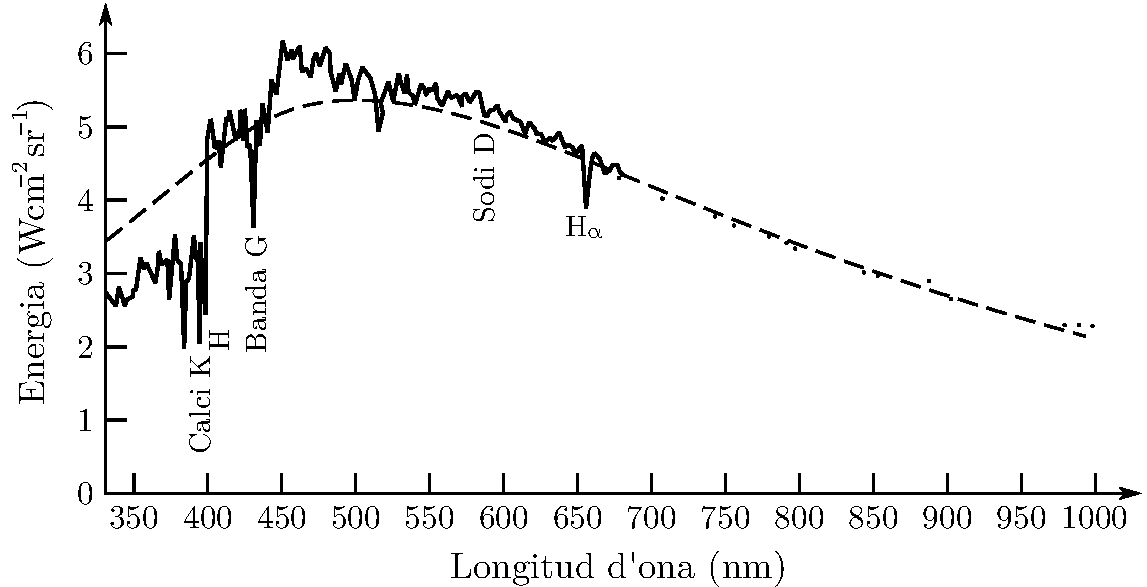
\includegraphics[width=0.8\textwidth]{./images/4-espectre-solar}
	\caption{Espectre solar}
	\label{fig:espectre-solar}
\end{figure}

La figura \ref{fig:espectre-solar} mostra l'espectre del Sol. La línia discontínua correspon a un cos negre de temperatura igual a la temperatura efectiva del Sol ($\SI{5770}{\K}$).

El decreixement de la intensitat a certes longituds d'ona es deu a l'absorció de la llum a aquestes longituds d'ona per metalls presents en l'atmosfera solar.

L'absorció es mesura mitjançant el \textit{coeficient d'absorció} o \textit{opacitat}, $\kappa_{\lambda}$.

Sigui un feix de llum, col·limat, que incideix sobre una placa de gas (figura \ref{fig:gas-opacitat}).
\begin{figure}[h]
	\centering
	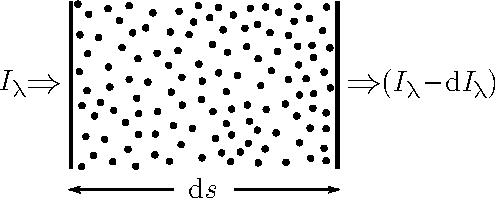
\includegraphics[width=0.45\textwidth]{./images/4-gas-opacitat}
	\caption{Placa de gas}
	\label{fig:gas-opacitat}
\end{figure}

La disminució d'intensitat al recórrer una distància $\dd{s}$ al gas de densitat $\rho$ és
\begin{align}\label{eq:int-opac}
	\dd{I}_{\lambda} = - \kappa_{\lambda} \rho I_{\lambda} \dd{s}
\end{align}
on $\kappa_{\lambda} > 0$ és la opacitat.

En general $\kappa_{\lambda}$ és una funció de la densitat del gas, la seva composició i temperatura. Al CGS té unitats de $\qty[\kappa_{\lambda}] = \si{\square\cm \per \g}$.

Convé advertir que en travesar el gas, es poden afegir fotons al feix per emissió dels àtoms de aquest gas. Així que l'equació \eqref{eq:int-opac} s'ha de generalitzar com
\begin{align}
	\dd{I}_{\lambda} = (j_{\lambda} - \kappa_{\lambda}) \rho I_{\lambda} \dd{s}
\end{align}
on $j_{\lambda}$ és el coeficient d'emissió del gas. De moment suposarem que $j_{\lambda} \equiv 0$.

Òbviament, si $\rho$ i $\kappa_{\lambda}$ són constants, l'equació \eqref{eq:int-opac} s'integra com
\begin{align}
	I_{\lambda}(s) = I_{\lambda 0} \exp[-\kappa_{\lambda} \rho s]
\end{align}

Així doncs, la distància típica que recorre un fotó qualsevol del feix abans d'abandonar-lo és
\begin{align*}
	l = \frac{1}{\kappa_{\lambda} \rho}
\end{align*}
aquesta és, a més a més, el \textit{recorregut lliure mig} dels fotons per procés de dispersió o \textit{scattering}.

\begin{example}
	En la fotosfera solar $\rho = \SI{2.5 e-7}{\g \per \cubic\cm}$, i la opacitat (per a $\lambda = \SI{5000}{\angstrom}$) $\kappa_{5000} = \SI{0.264}{\square\cm \per \g}$ , de manera que $l = \SI{1.52 e7}{\cm} = \SI{152}{\km}$.
\end{example}

%-----------------------------------------------------------------
\subsection{Profunditat òptica}
La profunditat òptica és un concepte unit estretament al d'opacitat. Quan observem la llum d'una estrella estem mirant al llarg del camí mitjà seguit pels fotons. Així doncs, es defineix profunditat òptica (\textit{optical depth}) com
\begin{align}\label{eq:opt-depth}
	\dd{\tau}_{\lambda} = - \kappa_{\lambda} \rho \dd{s}
\end{align}
on $s$ és la distància mesurada al llarg del camí del feix de llum en la direcció del moviment. Òbviament $\tau_{\lambda}$ és adimensional. Es pot veure que
\begin{align*}
	\Delta \tau_{\lambda} = \tau_{\lambda} - \tau_{\lambda 0} = - \int \kappa_{\lambda} \rho \dd{s}
\end{align*}
de manera que $\Delta \tau_{\lambda} < 0$.

Conforme la llum s'apropa a l'observador, aquesta viatja a través de valors més i més petits de $\tau_{\lambda}$. En les capes més externes de les estrelles $\tau_{\lambda} = 0$ ($\forall \lambda$). Així doncs,
\begin{align}
	\tau_{\lambda 0} = \int_{0}^{s} \kappa_{\lambda} \rho \dd{s}
\end{align}
és la profunditat òptica al llarg del raig en la seva posició inicial a la distància $s$ mesurada des de la superfície de l'atmosfera estel·lar.

Combinant \eqref{eq:int-opac} i \eqref{eq:opt-depth} i integrant s'obté
\begin{align}\label{eq:itau}
	I_{\lambda} = I_{\lambda 0} \exp[-\tau_{\lambda}]
\end{align}
de manera que la intensitat de llum decau exponencialment un cop abandona la superfície de l'estrella (sota la suposició que $\kappa_{\lambda}$ i $\rho$ són uniformes al llarg del camí seguit pel raig de llum).

Es pot veure que la profunditat òptica ens dóna el nombre de recorreguts lliures mitjos des de la superfície de l'estrella ($s > 0$) fins l'observador ($s = 0$):
\begin{align}
	l = \frac{1}{\kappa_{\lambda} \rho} \Rightarrow \tau_{\lambda} = \int_{0}^{s} \frac{\dd{s}}{l}
\end{align}
Ja que $\tau_{\lambda}$ depèn de $\lambda$, una atmosfera (o gas) pot ser òpticament gruixuda per a certes longituds d'ona i prima per a unes altres:
\begin{itemize}
	\item Si $\tau_{\lambda} \gg 1$, l'atmosfera es diu òpticament gruixuda (\textit{optically thick}).
	\item Si $\tau_{\lambda} \ll 1$, l'atmosfera es diu òpticament prima (\textit{optically thin}).
\end{itemize}

\begin{example}
	És obvi que les mesures del flux radioactiu rebut d'una estrella així com la magnitud aparent, $m$, han de ser corregides tenint en compte l'espessor de l'atmosfera terrestre.
	\begin{figure}[h]
		\centering
		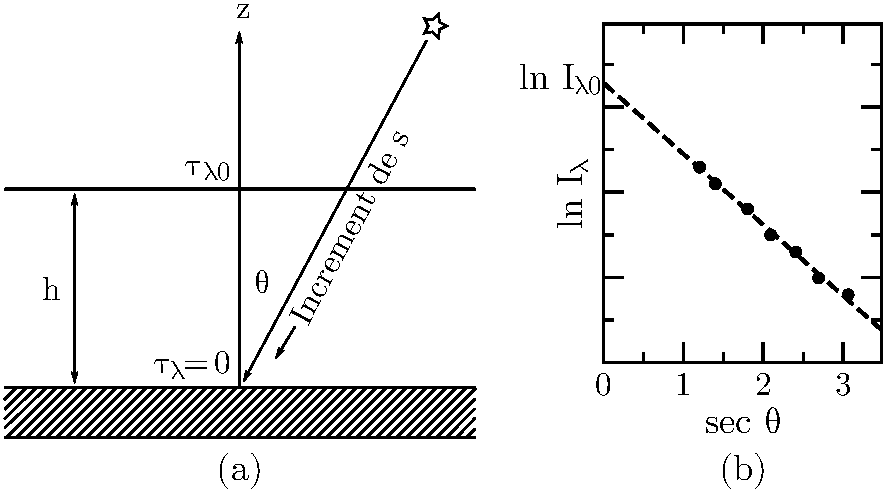
\includegraphics[width=0.6\textwidth]{./images/4-profunditat}
		\caption{(a) Un raig de llum entrant l'atmosfera terrestre amb un angle $\theta$, (b) $\ln I_{\lambda}$ en funció de $\sec \theta$}
		\label{fig:profunditat}
\end{figure}

	La figura \ref{fig:profunditat} mostra un raig que penetra en l'atmosfera terrestre sota un angle $\theta$ amb la vertical i viatjant fins un telescopi. L'alçada de l'atmosfera és $h$. La intensitat de la llum detectada al telescopi és $I_{\lambda}$.

	Es tracta de determinar $I_{\lambda 0}$. Per això considerem $\tau_{\lambda} = 0$ al telescopi (alçada zero), llavors
	\begin{align*}
		\tau_{\lambda} = \int_{0}^{s} \kappa_{\lambda} \rho \dd{s} = - \int_{0}^{h} \kappa_{\lambda} \rho \frac{\dd{z}}{\cos \theta} = \sec \theta \int_{0}^{h} \kappa_{\lambda} \rho \dd{z}
	\end{align*}
	Així doncs, $\tau_{\lambda} = \tau_{\lambda 0} \sec \theta$, de manera que
	\begin{align}
		I_{\lambda} = I_{\lambda 0} \exp[-\tau_{\lambda 0} \sec \theta]
	\end{align}
	però ens falta conèixer $I_{\lambda 0}$ i $\tau_{\lambda 0}$.

	Cap d'elles es pot determinar mitjançant una única observació. No obstant això, conforme la Terra gira en torn al seu eix, $\theta$ canvia, podent-se obtenir una gràfica (com a la figura \ref{fig:profunditat}) de $\ln I_{\lambda}$ en funció de $\sec \theta$.

	El pendent de la recta de regressió és $-\tau_{\lambda 0}$, i extrapolant la reca a $\sec \theta = 0$ s'obté gràficament $\ln I_{\lambda 0}$. Així es pot corregir la intensitat de flux radiant de l'absorció patida en travessar l'atmosfera terrestre.
\end{example}

%-----------------------------------------------------------------
\subsection{Fonts microscòpiques de l'opacitat}
Existeixen quatres processos principals que eliminen fotons d'un feix de llum mitjançant la interacció del fotó amb un electró (ja sigui aquest lliure o lligat, bé a un àtom neutre o a un ió):
\begin{figure}[h]
	\centering
	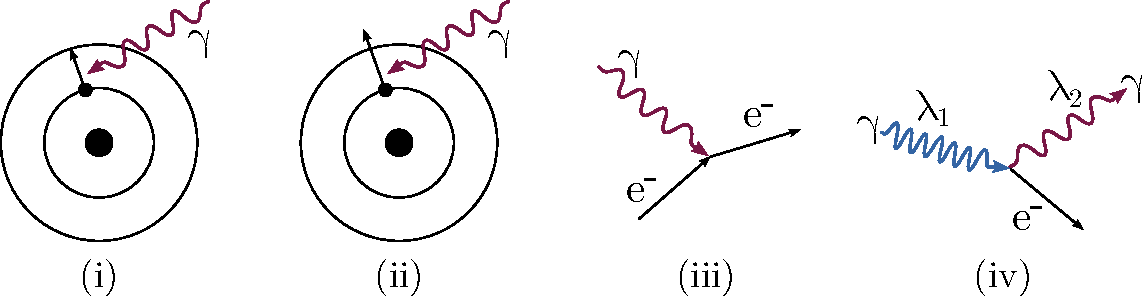
\includegraphics[width=0.8\textwidth]{./images/4-fonts-opacitat}
	\caption{(i) Transició lligat--lligat, (ii) transició lligat--lliure, (iii) absorció lliure--lliure, (iv) dispersió electrònica}
	\label{fig:fonts-opacitat}
\end{figure}

\begin{enumerate}[(i)]
	\item Transició lligat--lligat ($\kappa_{\lambda, bb}$): responsable de les ratlles d'absorció als espectres.
	\item Transició lligat--lliure ($\kappa_{\lambda, bf}$): font d'opacitat contínua, ja que pot eliminar del feix qualsevol fotó amb energia igual o superior a la d'ionització.
	\item Absorció lliure--lliure ($\kappa_{\lambda, ff}$): es tracta d'un procés de dispersió. Un electró lliure pròxim a un ió absorbeix un fotó i augmenta la seva velocitat. També contribueix a la opacitat contínua.

	El procés invers ($e^{-} \to e^{-} + \gamma$) rep el nom de \textit{Bremsstrahlung}.
	\item Dispersió electrònica ($\kappa_{es}$).
	\begin{enumerate}[(a)]
	\item Dispersió de Thomson: el fotó és dispersat per un electró lliure.

		És independent de $\lambda$ i és especialment eficaç a altes temperatures (la major part dels electrons són lliures a temperatures prou elevades). Aquest procés també contribueix a l'opacitat contínua.

		La secció eficaç de Thomson és
		\begin{align}
			\sigma_{T} = \frac{8\pi}{3} \qty(\frac{e^{2}}{m_{e} c^{2}}) = \SI{6.652 e-25}{\square\cm}
		\end{align}
		\item Dispersió de Compton: es dóna entre un fotó i un electró feblement lligat a un nucli atòmic si $\lambda \ll$ mida de l'àtom. També contribueix a l'opacitat contínua.
		\item Dispersió de Rayleigh: es dóna entre un fotó i un electró feblement lligat a un nucli atòmic si $\lambda \gg$ mida de l'àtom.

		La secció eficaç de Rayleigh és
		\begin{align}
			\sigma_{R} \propto \frac{1}{\lambda^{4}}
		\end{align}
		En la major part de les atmosferes estel·lars la dispersió de Rayleigh es pot menysprear. També contribueix a l'opacitat contínua.

		La dispersió de Rayleigh és responsable del color blau de la nostra atmosfera.
	\end{enumerate}
\end{enumerate}
És important senyalar que la font primària d'opacitat contínua en la majoria d'atmosferes estel·lars és la fotoionització d'ions \ch{H-} (un àtom format per $1p$ i $2e^{-}$). L'energia d'enllaç de l'electró addicional és $B = \SI{0.75}{\eV}$, de manera que qualsevol fotó amb $\lambda \leq hc/B = \SI{16400}{\angstrom}$ pot ser absorbit i l'electró alliberat.

Així doncs, aquest procés és una font important d'opacitat contínua des de la meitat de l'infraroig a longituds d'ona menors.

%-----------------------------------------------------------------
\subsection{Opacitat total}
L'opacitat total és la suma de totes les opacitats i depèn no només de la longitud d'ona sinó també de la composició, densitat i temperatura de l'atmosfera estel·lar:
\begin{align}
	\kappa_{\lambda} = \kappa_{\lambda, bb} + \kappa_{\lambda, bf} + \kappa_{\lambda, ff} + \kappa_{es}
\end{align}

\subsubsection*{Opacitat mitjana de Rosseland}
És l'opacitat obtinguda de fer la mitjana sobre $\lambda$, de manera que noés deoèn de la densitat, composició, i temperatura de l'atmosfera estel·lar. Així doncs, tenim $\bar{\kappa}_{\lambda, bb}$, $\bar{\kappa}_{\lambda, bf}$, $\bar{\kappa}_{\lambda, ff}$, i $\bar{\kappa}_{es}$.

L'opacitat total de Rosseland total és
\begin{align}
	\bar{\kappa} = \overline{\kappa_{\lambda, bb} + \kappa_{\lambda, bf} + \kappa_{\lambda, ff} + \kappa_{es}}
\end{align}
\begin{figure}[h]
	\centering
	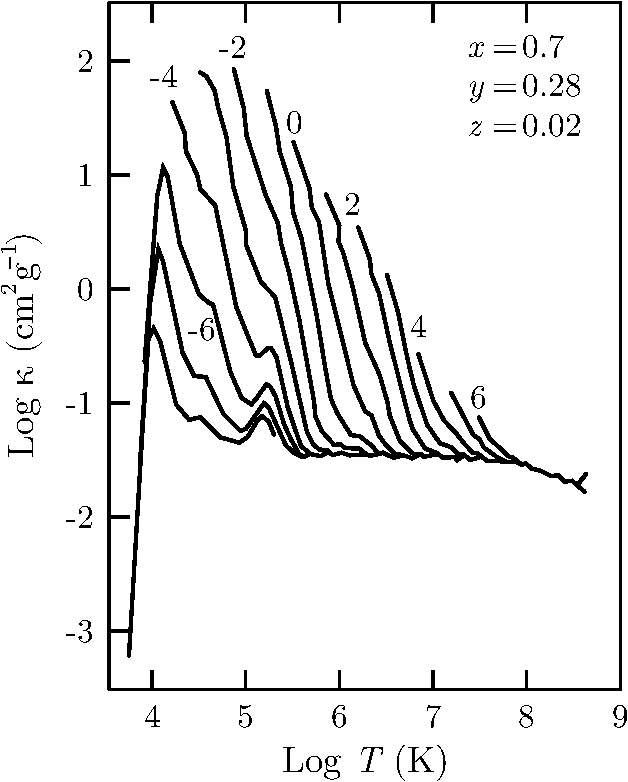
\includegraphics[width=0.45\textwidth]{./images/4-opacitat-rosseland}
	\caption{Opacitat mitjana de Rosseland. Les corbes estan etiquetades per $\log \rho$ en $\si{\g \per \cubic\cm}$}
	\label{fig:opacitat-rosseland}
\end{figure}

La figura \ref{fig:opacitat-rosseland} mostra $\bar{\kappa}$ en funció de la temperatura, amb $x = 0.7$, $y = 0.28$, $z = 0.02$ (on $x$, $y$, $z$ són les fraccions en pes d'hidrogen, heli i metalls, respectivament).

Inicialment $\bar{\kappa}$ creix quasi verticalment amb $T$ a causa del gran nombre d'electrons lliures procedents d'àtoms d'hidrogen i heli. Després d'assolir un màxim, les corbes cauen seguint aproximadament la llei de Kramers
\begin{align}
	\bar{\kappa} \propto T^{-3.5}
\end{align}
a causa de les absorcions lliure--lliure i lligat--lliure.

L'ió \ch{He} perd el seu únic electró aproximadament a $\SI{40000}{\K}$. Aquest lleuger augment d'electrons produeix el pic que s'observa en torn a aquesta temperatura.

En la zona inferior dreta de la figura, els gràfics posseeixen pendent nul. Allí domina l'absorció per dispersió d'electrons ja que a altes temperatures tots els electrons són lliures.
%-----------------------------------------------------------------
\subsection{Extinció}
La presència de pols i gas ocasiona que ens arribi menys llum de la que ens hauria arribat en absència d'aquests. Això, a més a més, provoca \textit{reddening}, l'empobriment de la llum en components  de curta longitud d'ona.

La quantificació sumultània d'ambdós efectes, ja que van units, es realitza mitjançant el paràmetre $A$. L'expressió $m - M = 5 \log(d/\SI{10}{\parsec})$ es converteix en
\begin{align}\label{eq:mMA}
	m - M = 5 \log(\frac{d}{\SI{10}{\parsec}}) + A
\end{align}
quan l'extinció (i/o reddening) es tenen en compte.

És obvi que si no hi hagués absorció (opacitat) es tindria $A = 0$ i la profunditat òptica seria $\tau = 0$.

\subsubsection*{Deducció de la relació entre $A$ i $\tau$}
Sigui $F_{0}$ el flux en la superfície d'una estrella de radi $R$, i $F(d)$ el seu valor a la distància $d$. Es pot veure que
\begin{align}\label{eq:iflux}
	I = \Omega F(d) d^{2} \Rightarrow I_{0} = \Omega F_{0} R^{2}
\end{align}
combinant \eqref{eq:itau} amb l'equació \eqref{eq:iflux} se segueix
\begin{align}
	F(d) = F_{0} \qty(\frac{R}{d})^{2} \exp[-\tau]
\end{align}
Per obtenir la distància mòdul, $m - M$, necessitem conèixer el flux que rebríem si l'estrella fos a $\SI{10}{\parsec} $ del nostre telescopi, avaluat sense extinció ($\tau = 0$):
\begin{align*}
	F(d) = F_{0} \frac{R^{2}}{(\SI{10}{\parsec})^{2}}
\end{align*}
La distància mòdul la podem escriure com
\begin{align*}
	m - M = -2.5 \log(\frac{F(d)}{F(\SI{10}{\parsec})}) = -2.5 \log[ \qty(\frac{\SI{10}{\parsec}}{d})^{2} \exp[-\tau]]
\end{align*}
és a dir
\begin{align}
	m - M = 5 \log(\frac{d}{\SI{10}{\parsec}}) + \qty(2.5 \log e) \tau
\end{align}
Comparant amb \eqref{eq:mMA}, obtenim
\begin{align}
	A_{\lambda} = \qty(2.5 \log e) \tau_{\lambda}
\end{align}
El subíndex $\lambda$ ens recorda que aquesta expressió és vàlida per a qualsevol longitud d'ona.

\begin{example}
	Cal trobar la profunditat òptica d'un banc de boira si el Sol vist a través d'aquest posseeix una lluminositat igual a la de la lluna plena en una nit perfecta. Dades: $m_{\odot} = -26.8$, $m_{L} = -12.5$.
	\begin{align*}
		A = m_{L} - m_{\odot} = \qty(2.5 \log e) \tau \Rightarrow \tau \approx 13.17
	\end{align*}
\end{example}

%-----------------------------------------------------------------
\subsection{Estructura de les línies espectrals}
La forma de la línia espectral conté una informació molt valuosa quant a l'ambient en què es va formar.
\begin{figure}[h]
	\centering
	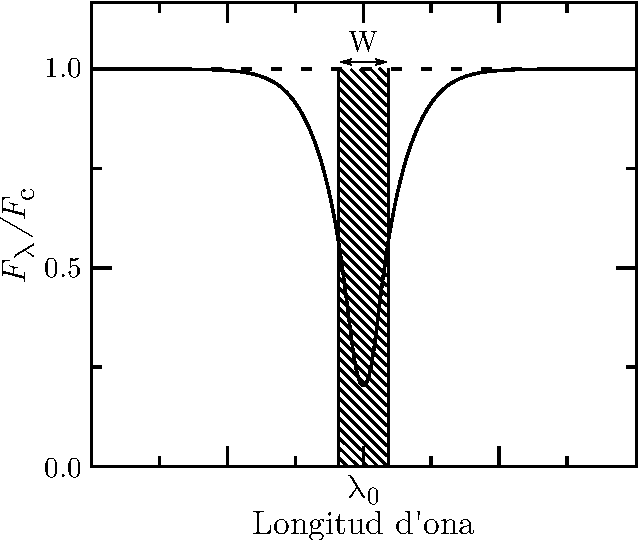
\includegraphics[width=0.5\textwidth]{./images/4-typical-spectral}
	\caption{Forma típica d'una línia espectral}
	\label{fig:typical-spectral}
\end{figure}

La figura \ref{fig:typical-spectral} mostra el flux radiant, $F_{\lambda}$, en funció de $\lambda$ per a una línia espectral típica.

La profunditat de la línia espectral és una funció de $\lambda$:
\begin{align}
	\frac{F_{c} - F_{\lambda}}{F_{c}}
\end{align}
on $F_{c}$ és el valor del flux radiant en l'espectre continu, i $\lambda_{0}$ la longitud d'ona al centre de la línia.

L'amplada de la línia (o amplada equivalent), $W$, sol ser $\approx \SI{0.1}{\angstrom}$:
\begin{align}
	W = \int \frac{F_{c} - F_{\lambda}}{F_{c}} \dd{\lambda}
\end{align}
Una altra mesura de l'amplada és l'amplada sencera a la meitat del màxim $(\Delta \lambda)_{1/2}$, és a dir, la distància de banda a banda de la línia espectral justament on se satisfà
\begin{align*}
	\frac{F_{c} - F_{\lambda}}{F_{c} - F_{\lambda 0}} = \frac{1}{2}
\end{align*}
En la figura \ref{fig:typical-spectral}, l'opacitat $\kappa_{\lambda}$ del material estel·lar és màxima en $\lambda_{0}$ (ja que allí l'absorció és màxima) i decreix conforme ens desplacem (a la dreta o esquerra de $\lambda_{0}$) pels costats de la línia espectral. Es pot concloure que el centre de la línia espectral (en $\lambda_{0}$) es va formar a les zones altes (i fredes) de l'atmosfera estel·lar. Conforme ens desplacem cap a dalt al llarg dels costats, aquests trams es van formar en zones més profundes i calents de l'atmosfera solar.

Hi ha tres efectes diferents que contribueixen a l'eixamplament de les línies espectrals.

\subsubsection*{Eixamplament natural}
Pel principi d'incertesa de Heisenberg, la incertesa en l'energia d'un electró en un orbital concret és
\begin{align*}
	\Delta E \approx \frac{\hbar}{\Delta t}
\end{align*}
on $\Delta t$ és l'interval de temps d'un electró en aquest orbital. Combinant aquesta equació amb
\begin{align*}
	E_{\gamma} = \frac{h c}{\lambda} \Rightarrow \dv{E}{\lambda} = - \frac{h c}{\lambda^{2}}
\end{align*}
arribem fàcilment a una expressió per l'eixamplament de les línies espectrals:
\begin{align}
	\Delta \lambda \approx \frac{\lambda^{2}}{2\pi c} \qty(\frac{1}{\Delta t_{i}} + \frac{1}{\Delta t_{f}})
\end{align}

\subsubsection*{Eixamplament per efecte Doppler}
En equilibri tèrmic, la velocitat més probable dels àtoms del gas és $v_{mp} = \sqrt{2 k_{B} T/m}$, i les longituds d'ona de la llum absorbida o emesa pels àtoms del gas seran desplaçades d'acord amb $\Delta \lambda / \lambda = \pm v_{r}/c$, de manera que
\begin{align}
	\Delta \lambda = \frac{2\lambda}{c} \sqrt{\frac{2 k_{B} T}{m}}
\end{align}
\begin{example}
	Per a àtoms d'hidrogen en la fotosfera solar ($T = \SI{5770}{\K}$) l'eixamplament per efecte Doppler de la línia $H_{\alpha}$ de l'hidrogen ($\lambda = \SI{6560.44}{\angstrom}$) resulta ser $\Delta \lambda = \SI{0.427}{\angstrom}$, aproximadament $\num{e3}$ vegades major que l'eixamplament natural.
\end{example}
Un estudi més detallat ens indica que l'eixamplament de la línia en la meitat del màxim és
\begin{align}
	(\Delta \lambda)_{1/2} = \frac{2\lambda}{c} \sqrt{\frac{2 k_{B} T}{m} \ln 2}
\end{align}
Si el moviment dels àtoms del gas és turbulent i la distribució de velocitats turbulentes segueix una distribució de Maxwell--Boltzmann, tenim
\begin{align}
	(\Delta \lambda)_{1/2} = \frac{2\lambda}{c} \sqrt{\qty[\frac{2 k_{B} T}{m} + v^{2}_{turb}] \ln 2}
\end{align}
Gràcies a aquest efecte es va poder inferir l'existència de fluxos turbulents en les atmosferes d'estrelles gegants i supergegants.

\subsubsection*{Eixamplament col·lisional i de pressió}
Col·lisions entre àtoms així com el camp elèctric d'un gran nombre d'ions passant a prop d'un àtom poden pertorbar els orbitals d'aquest.

Sense entrar en detalls de càlcul, es veu que l'eixamplament de les línies espectrals ve donat per
\begin{align}
	\Delta \lambda \approx \frac{\lambda^{2}}{c} \frac{n \sigma}{c} \sqrt{\frac{2 k_{B} T}{m}}
\end{align}
on $n$ és la densitat numèrica d'àtoms, i $\sigma$ és la secció eficaç de col·lisió.
\begin{example}
	Per a àtoms d'hidrogen en la fotosfera solar ($T = \SI{5770}{\K}$) l'eixamplament col·lisional i de pressió de la línia $H_{\alpha}$ de l'hidrogen ($\lambda = \SI{6560.44}{\angstrom}$) resulta ser $\Delta \lambda = \SI{2.36 e-4}{\angstrom}$, valor similar a l'eixamplament natural.
\end{example}

%-----------------------------------------------------------------
%	ESTRELLES BINÀRIES
%	!TEX root = ./../main.tex
%-----------------------------------------------------------------
\section{Estrelles binàries}
Aproximadament la meitat de les estrelles són sistemes de dos o més components que orbiten en torn a un centre de massa comú. Aquí considerarem només sistemes binaris.

Aquests sistemes es poden classificar segons les seves característiques observacionals. Els diferents grups d'aquesta classificació no són, però, mútuament excloents; així doncs, un sistema binari pot ser a la vegada eclipsant i espectroscòpica.

\subsection{Classificació dels sistemes binaris}
\subsubsection*{Binàries òptiques}
Dues estrelles que jeuen en la mateixa visual no lligades gravitacionalment entre si (ja que estan molt lluny l'una de l'altra), de manera que no formen un autèntic sistema binari.

\subsubsection*{Binàries visuals}
Ambdues estrelles poden resoldre's individualment, i si el període orbital no és molt llarg, és possible seguir el moviment de cadascuna.

Si, a més, la distància al sistema binari és coneguda, la separació entre ambdues estrelles es podrà determinar.

\subsubsection*{Binàries astromètriques}
Si un membre del sistema és molt més brillant que l'altre membre, això no es podrà observar visualment.
\begin{figure}[h]
	\centering
	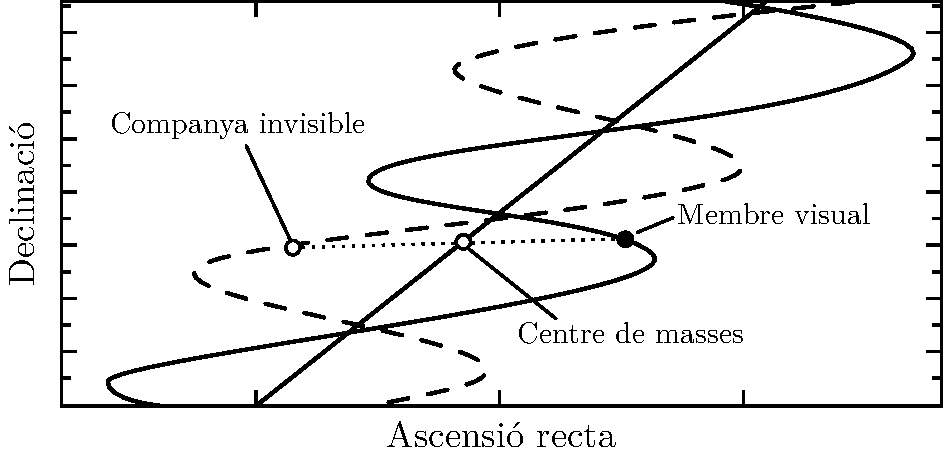
\includegraphics[width=0.7\textwidth]{./images/5-bin-astro}
	\caption{Diagrama de la dinàmica d'un sistema binari astromètric}
	\label{fig:bin-astro}
\end{figure}

No obstant, la seva existència es pot deduir del moviment oscil·latori del primer (figura \ref{fig:bin-astro}).

\subsubsection*{Binàries eclipsants}
Si el pla d'òrbita està orientat aproximadament al llarg de la visual de l'observador terrestre, una estrella passarà periòdicament en front de l'altra interceptant la llum d'aquesta (es produeix un eclipsi).
\begin{figure}[h]
	\centering
	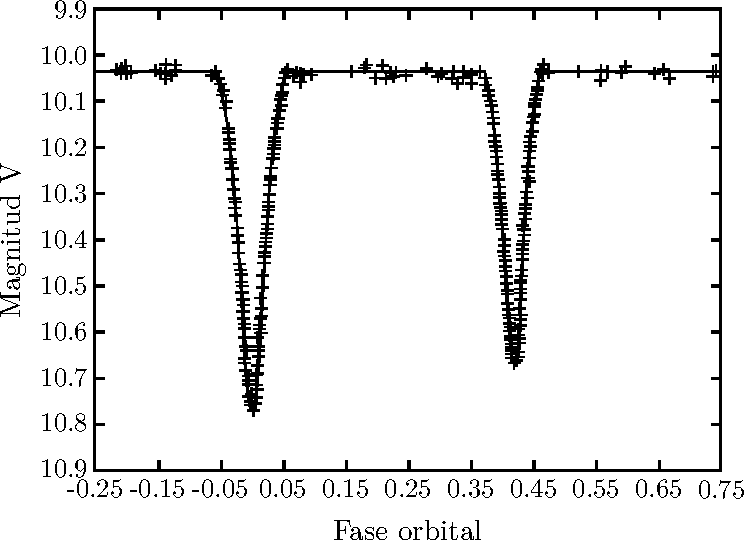
\includegraphics[width=0.7\textwidth]{./images/5-bin-eclip}
	\caption{Corba de llum del sistema YY Sagitari de període \num{2.6284734} dies, excentricitat $\num{0.1573}$, i inclinació orbital $i = \SI{88.89}{\degree}$}
	\label{fig:bin-eclip}
\end{figure}

S'infereix l'existència d'aquests sistemes per la variació periòdica en la llum rebuda al telescopi terrestre (figura \ref{fig:bin-eclip}).

La corresponent corba de la llum proporciona, a més, informació quant al quocient entre les temperatures d'ambdues estrelles, i dels seus radis.

\subsubsection*{Binàries espectrals}
És un sistema amb dos espectres independents, discernibles i superposats. Quan l'espectre d'una estrella està desplaçat cap al vermell, el de l'altra ho està cap al blau i viceversa (respecte de l'espectre que tindrien si es moguessin amb la velocitat constant del centre de masses).

\subsubsection*{Binàries espectroscòpiques}
Si el període del sistema no és molt gran i si el moviment en l'òrbita té una component al llarg de la visual, s'observarà un desplaçament periòdic de les línies espectrals.
\begin{figure}[h]
	\centering
	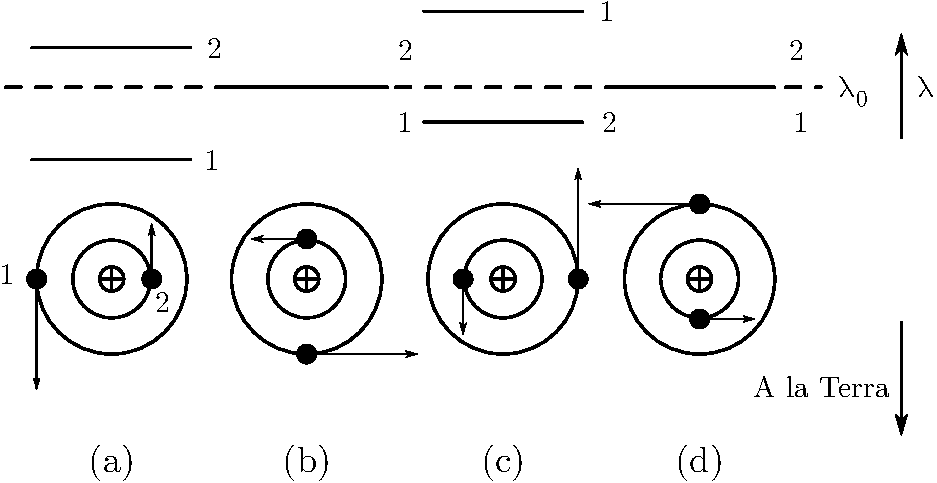
\includegraphics[width=0.8\textwidth]{./images/5-bin-spect}
	\caption{Desplaçament periòdic de les línies espectrals d'un sistema binari espectroscòpic}
	\label{fig:bin-spect}
\end{figure}

Si ambdues estrelles són de lluminositat semblant, ambdós espectres seran observables. No obstant això, si una estrella és molt més lluminosa que l'altra, l'espectre de la menys lluminosa no serà discernible i només seran visibles les línies espectrals de la primera.

Tant en un cas com en l'altre tenim un sistema binari. La figura \ref{fig:bin-spect} il·lustra la relació entre els espectres i les fases orbitals.


%-----------------------------------------------------------------
\subsection{Determinació de les masses d'un sistema binari}
\subsubsection*{Determinació de les masses d'un sistema binari visual}
Aquí ambdues estrelles es distingeixen visualment l'una de l'altra. Prenent l'origen de coordenades al centre de masses ($CM$), tenim
\begin{align}\label{eq:bin-ma}
	\frac{m_{1} \va{r}_{1} + m_{2} \va{r}_{2}}{m_{1} + m_{2}} = \va{0} \Rightarrow \frac{m_{1}}{m_{2}} = \frac{r_{2}}{r_{1}} = \frac{a_{2}}{a_{1}}
\end{align}
on $\norm{\va{r}_{i}} = r_{i} = a_{i}$ és el semieix major de les òrbites el·lipsoïdals de les estrelles.

Els angles subtendits pels semieixos seran (en radiants) $\alpha_{i} = a_{i} / d$, on $d$ és la distància del sistema binari a l'observador. Substituint en l'equació \eqref{eq:bin-ma} es pot determinar el quocient entre les masses:
\begin{align}\label{eq:bin-malpha}
	\frac{m_{1}}{m_{2}} = \frac{\alpha_{2}}{\alpha_{1}}
\end{align}
Les masses individuals també es poden obtenir. Només cal utilitzar l'equació \eqref{eq:bin-malpha} amb la tercera llei de Kepler:
\begin{align}\label{eq:bin-mkepler}
	T^{2} = \frac{4\pi^{2}}{G} \frac{a^{3}}{m_{1} + m_{2}}
\end{align}
on $a = a_{1} + a_{2}$ és el semieix major de l'òrbita de la massa reduïda.

Fins aquí hem suposat que:
\begin{enumerate}[(i)]
	\item El moviment del $CM$ es pot sostreure sense dificultat.
	\item El pla de les òrbites és perpendicular a la visual.
\end{enumerate}
Quan (ii) no es compleix, hi haurà un angle (que anomenarem $i$) entre el pla de les òrbites i el pla del cel (aquest és perpendicular a la visual).
\begin{figure}[h]
	\centering
	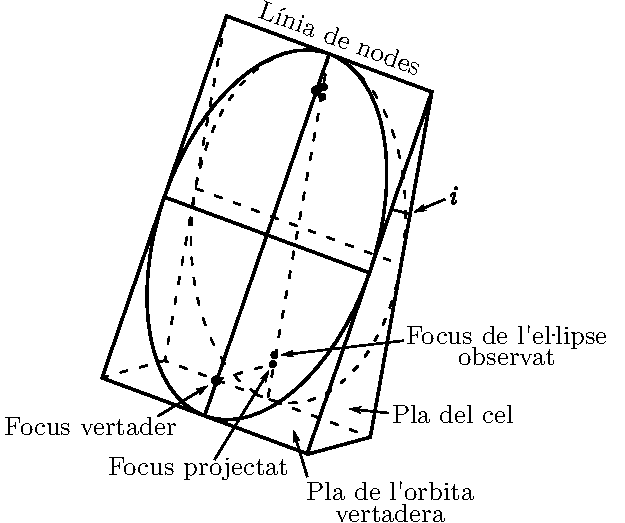
\includegraphics[width=0.6\textwidth]{./images/5-bin-visual-pla}
	\caption{L'òrbita observada és en realitat l'òrbita vertadera projectada sobre el pla del cel}
	\label{fig:bin-visual-pla}
\end{figure}

A la figura \ref{fig:bin-visual-pla} s'ha suposat que la línia de la intersecció d'ambdós plans és paral·lela al semieix menor (cal recordar, de pas, que les òrbites d'ambdues estrelles jeuen sobre el mateix pla).

L'observador terrestre no mesura en realitat $\alpha_{1}$ i $\alpha_{2}$, sinó que la seva projecció sobre el pla del cel: $\tilde{\alpha_{i}} = \alpha_{i} \cos i$. Llavors, en comptes de l'equació \eqref{eq:bin-malpha}, tenim la seva equivalent
\begin{align}
	\frac{m_{1}}{m_{2}} = \frac{\tilde{\alpha}_{2}}{\tilde{\alpha}_{1}}
\end{align}
Tenint en compte que
\begin{align*}
	a = \alpha d = \frac{\tilde{\alpha}}{\cos i} d
\end{align*}
on $\tilde{\alpha} = \tilde{\alpha}_{1} + \tilde{\alpha}_{2}$, en comptes de l'equació \eqref{eq:bin-mkepler} ara tenim
\begin{align}
	T^{2} = \frac{4\pi^{2}}{G} \frac{(\tilde{\alpha}/\cos i)^{3}}{m_{1} + m_{2}} d^{3}
\end{align}
Veiem, doncs, que l'angle $i$ efectivament intervé en la determinació de les masses, i aquest s'ha d'obtenir esbrinant la posició aparent del $CM$ sobre el pla del cel.

Fins i tot en el cas en què la distància $d$ al sistema binari sigui desconeguda és possible trobar $m_{1}$ i $m_{2}$. Per això es necessita conèixer la projecció dels vectors velocitat d'ambdues estrelles sobre la visual. Això, juntament amb la informació quant a les posicions de les estrelles i l'orientació de les seves òrbites, permet esbrinar els semieixos majors d'ambdues òrbites.

%-----------------------------
\subsubsection*{Determinació de les masses d'un sistema espectroscòpic binari}
En aquest cas tenim desplaçaments Doppler periòdics de les línies espectrals d'ambdós components del sistema.
\begin{itemize}
	\item Si les òrbites són circulars, la velocitat de cada estrella serà constant.
	\item Si la visual pertany al pla de les òrbites ($i = \SI{\pi/2}{\radian}$), la component radial de la velocitat observada serà sinusoïdal (figura \ref{fig:bin-spect-sinus}).
\end{itemize}
\begin{figure}[h]
	\centering
	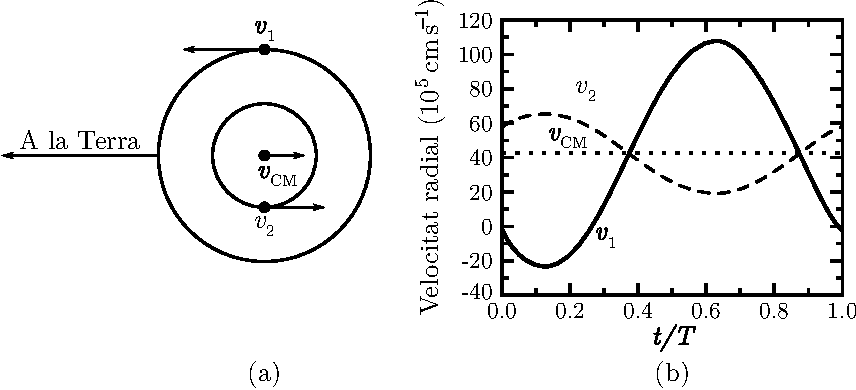
\includegraphics[width=0.8\textwidth]{./images/5-bin-spect-sinus}
	\caption{(a) Dues òrbites circulars el pla de les quals conté la visual de l'observador, (b) corbes de les velocitats radials observades d'ambdues estrelles i del $CM$}
	\label{fig:bin-spect-sinus}
\end{figure}

\begin{itemize}
	\item Si $i \neq \SI{\pi/2}{\radian}$ (la visual ja no pertany al pla de les òrbites) les amplituds queden multiplicades per un factor $\sin i$, però la forma de les corbes no canvia.
	\item Si les òrbites no són circulars (excentricitat $e \neq 0$), les corbes de velocitat observades resultes inclinades (figura \ref{fig:bin-spect-eneq0}) i la forma d'aquestes depèn de l'angle $i$.
\end{itemize}
\begin{figure}[h]
	\centering
	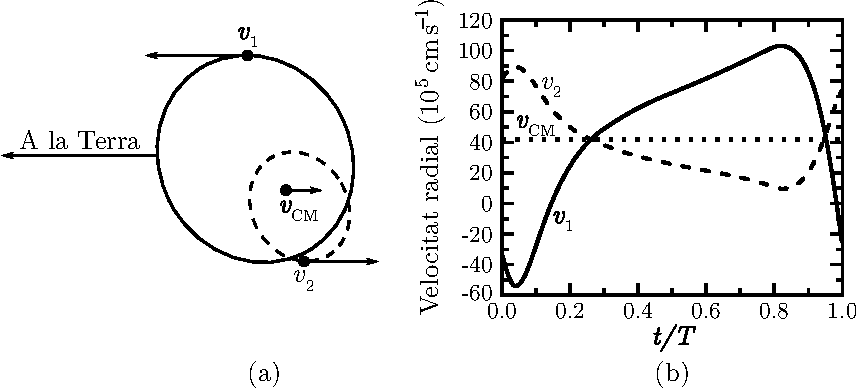
\includegraphics[width=0.8\textwidth]{./images/5-bin-spect-eneq0}
	\caption{Velocitats radials observades. En aquest cas $m_{1} = \SI{0.5}{\Msun}$, $m_{2} = \SI{2.0}{\Msun}$, $a = \SI{2}{\au}$, $e = 0.3$, $i = \SI{\pi/6}{\radian}$}
	\label{fig:bin-spect-eneq0}
\end{figure}

Ja que en realitat moltes binàries posseeixen òrbites de baixa excentricitat suposarem òrbites circulars:
\begin{align*}
	v_{i} = \frac{2\pi a_{i}}{T}
\end{align*}
Utilitzant l'equació \eqref{eq:bin-ma} se segueix
\begin{align}\label{eq:bin-mmvv}
	\frac{m_{1}}{m_{2}} = \frac{v_{2}}{v_{1}}
\end{align}
A més a més, $v_{1 r} = v_{1} \sin i$ i $v_{2 r} = v_{2} \sin i$, de manera que
\begin{align}\label{eq:bin-mmvrvr}
	\frac{m_{1}}{m_{2}} = \frac{v_{2 r}}{v_{1 r}}
\end{align}
Així doncs, el quocient entre ambdues velocitats radials observades ens dóna el quocient entre les masses.

Per determinar la suma de les masses utilitzem l'equació \eqref{eq:bin-mkepler} (Kepler), de manera que
\begin{align}\label{eq:bin-mkepler2}
	m_{1} + m_{2} = \frac{T}{2\pi G} \frac{(v_{1 r} + v_{2 r})^{3}}{\sin^{3} i}
\end{align}
Així doncs, hem de conèixer les components radials de la velocitat d'ambdues estrelles.

Amb freqüència una estrella (e.g., la 1) és molt més brillant que l'altra, de forma que l'espectre d'aquesta resulta inaccessible. En aquest cas només es coneix $v_{1 r}$ i no és possible determinar les masses individuals. No obstant, utilitzant la relació \eqref{eq:bin-mmvrvr} per eliminar $v_{2 r}$ de l'equació \eqref{eq:bin-mkepler2}, tenim:
\begin{align*}
	m_{1} + m_{2} = \frac{T}{2\pi G} \frac{v_{1 r}^{3}}{\sin^{3} i} \qty(1 + \frac{m_{1}}{m_{2}})^{3}
\end{align*}
i després de reordenar els termes obtenim
\begin{align}\label{eq:bin-mkepler3}
	\frac{m_{2}^{3}}{(m_{1} + m_{2})^{2}} \sin^{3} i = \frac{T}{2\pi G} v_{1 r}^{3}
\end{align}

El costat dret de l'expressió \eqref{eq:bin-mkepler3} es coneix com la \textit{funció de massa}, i depèn només de les magnituds obtingudes mitjançant l'observació (període i velocitat radial de l'estrella 1).
\begin{figure}[h]
	\centering
	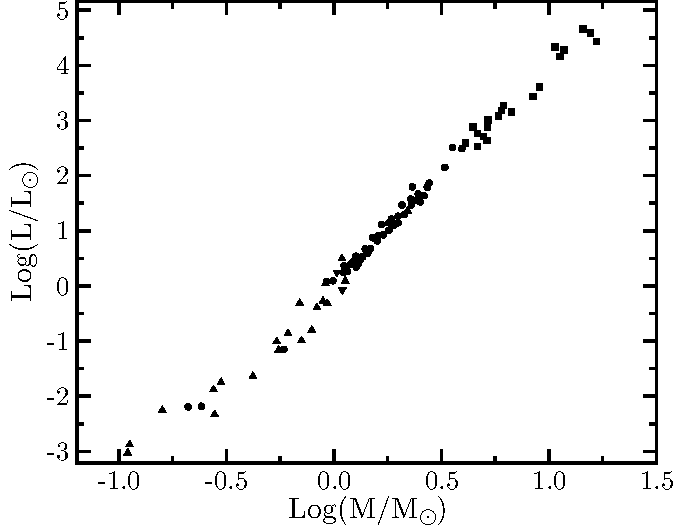
\includegraphics[width=0.6\textwidth]{./images/5-bin-spect-m-l}
	\caption{Relació massa--lluminositat. ($\bullet$) Sistemes de la seqüència principal distants, B6 fins M, ($\blacktriangle$) binàries visuals, (${\scriptstyle \blacksquare}$) sistemes OB distants, ($\blacktriangledown$) binàries espectroscòpiques resoltes}
	\label{fig:bin-spect-m-l}
\end{figure}

Ja que no és es coneix l'espectre de l'estrella 1, no és possible determinar $m_{1} / m_{2}$. En conseqüència, la funció de massa és útil només per a estudis estadístics o si una estimació de la massa d'un dels components fos possible per mètodes indirectes.

Si $m_{1}$ o bé $\sin i$ fos desconegut, la funció de massa imposa un límit sobre $m_{2}$, ja que el costat esquerre de l'equació \eqref{eq:bin-mkepler3} és inferior a $m_{2}$.

Gràcies a la determinació de masses en sistemes binaris s'ha aconseguit obtenir una relació empírica massa--lluminositat per a la majoria de les estrelles del firmament (figura \ref{fig:bin-spect-m-l}).

%-----------------------------
\subsubsection*{Determinació de les masses d'un sistema espectroscòpic binari eclipsant}
Si el sistema espectroscòpic binari és a més eclipsant, es pot obtenir informació addicional.
\begin{figure}[H]
	\centering
	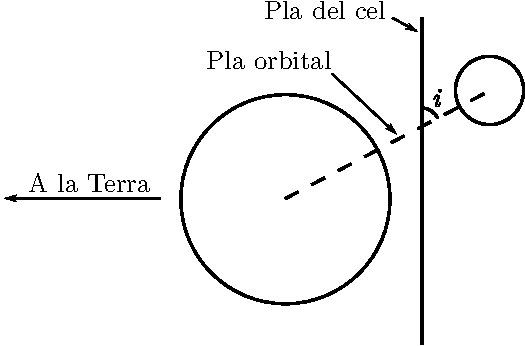
\includegraphics[width=0.5\textwidth]{./images/5-bin-pi2}
	\caption{Geometria d'una binària espectroscòpica eclipsant requereix que l'angle d'inclinació sigui $i \approx \SI{\pi/2}{\radian}$}
	\label{fig:bin-pi2}
\end{figure}

En primer lloc, l'angle $i$ entre el pla de les òrbites i el pla cel cel ha de ser pròxim a $\SI{\pi/2}{\radian}$ (figura \ref{fig:bin-pi2}).

La duració dels eclipsis permet estimar els radis d'ambdues estrelles. Per simplificar\footnote{Cal notar, que en el desenvolupament hem menyspreat l'efecte dels llimbs i la possible no esfericitat de les estrelles a causa de la presència de l'altra.} el desenvolupament, suposem que $i \equiv \SI{\pi/2}{\radian}$.
\begin{figure}[h]
	\centering
	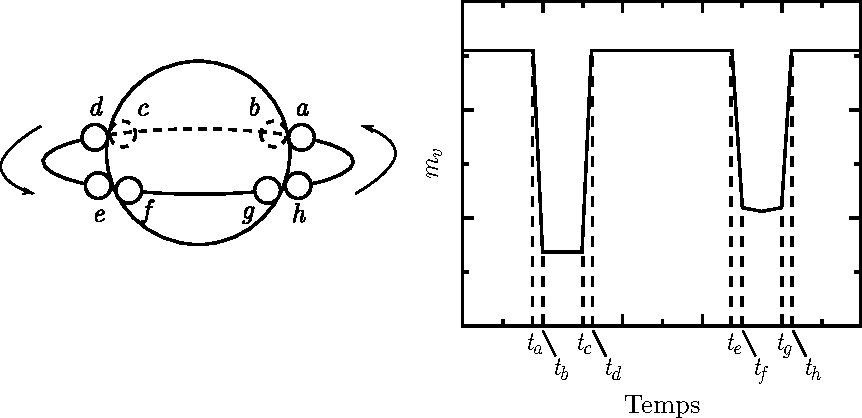
\includegraphics[width=0.8\textwidth]{./images/5-bin-eclipses}
	\caption{Corba de llum d'una binària eclipsant amb $i = \SI{\pi/2}{\radian}$. Els temps indicats en l'eix de les abscisses corresponen a les posicions successives de l'estrella petita respecte a la gran. Entre $t_{b}$ i $t_{c}$ la petita es troba totalment oculta per la gran. Aquí se suposa implícitament que la petita és de major temperatura que la gran}
	\label{fig:bin-eclipses}
\end{figure}

De la figura \ref{fig:bin-eclipses}, deduïm que el radi de l'estrella petita és donat aproximadament per
\begin{align}
	r_{s} = \frac{1}{2} v (t_{b} - t_{a})
\end{align}
i deduïm que el radi de l'estrella gran és aproximadament
\begin{align}
	r_{l} = \frac{1}{2} v (t_{c} - t_{a})
\end{align}
on $v = v_{s} + v_{l}$ és la velocitat relativa d'ambdues estrelles.

El flux de radiació en la superfície (de cada estrella) ve donat per
\begin{align}\label{eq:F-T}
   F = \sigma T_{e}^{4}
\end{align}

Suposem que l'estrella de major temperatura és la petita. Referint-nos de nou a la figura \ref{fig:bin-eclipses}, la brillantor quan ambdues estrelles són totalment visibles és
\begin{align}
	B_{0} = k (\pi r_{l}^{2} F_{l} + \pi r_{s}^{2} F_{s}) \qc (k > 0)
\end{align}
En el primer mínim (el més profund $\Rightarrow$ estrella petita oculta) la brillantor serà
\begin{align*}
	B_{p} = k \pi r_{l}^{2} F_{l}
\end{align*}
En el segon mínim (estrella gran parcialment oculta), la brillantor serà
\begin{align*}
	B_{s} = k (\pi r_{l}^{2} - \pi r_{s}^{2}) F_{l} + k \pi r_{s}^{2} F_{s}
\end{align*}
Com que la constant $k$ no es pot determinar amb prou exactitud hem de conformar-nos amb el quocient
\begin{align*}
	\frac{B_{0} - B_{p}}{B_{0} - B_{s}} = \frac{F_{s}}{F_{l}}
\end{align*}
i utilitzant l'equació \eqref{eq:F-T}, obtenim
\begin{align}
	\frac{B_{0} - B_{p}}{B_{0} - B_{s}} = \qty(\frac{T_{s}}{T_{l}})^{4}
\end{align}

\setcounter{section}{11}
%-----------------------------------------------------------------
%	LA NOSTRA GALÀXIA: LA VIA LÀCTIA
%	!TEX root = ./../main.tex
%-----------------------------------------------------------------
\section{La nostra galàxia: la Via Làctia}
\subsection{Forma i mida de la Via Làctia}
La majoria d'estrelles visibles a simple vista de la nostra galàxia (la Via Làctia, o simplement la Galàxia) es troba en un gegant disc prim (figura \ref{fig:disc}).
\begin{figure}[h]
	\centering
	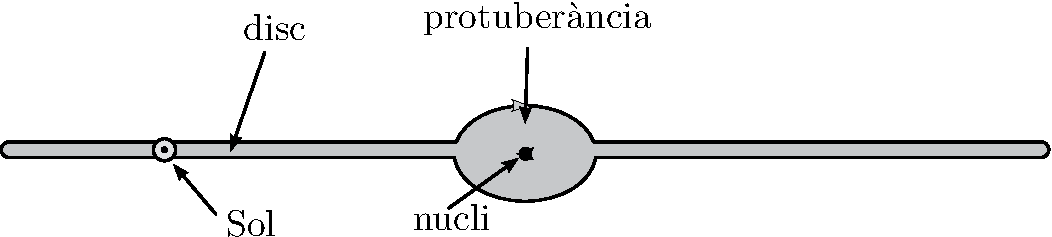
\includegraphics[width=0.7\textwidth]{./images/6-disc}
	\caption{La nostra posició a la Galàxia. Som al centre del disc, però més lluny del centre de la Galàxia que de l'extrem del disc}
	\label{fig:disc}
\end{figure}

El disc el veiem de cantonada, ja que ens trobem en ell; a l'estiu (hemisferi nord), destaca més que a l'hivern (figura \ref{fig:disc-nord-sud}).
\begin{figure}[h]
	\centering
	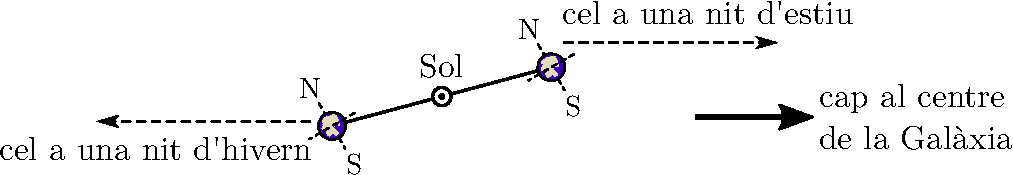
\includegraphics[width=0.8\textwidth]{./images/6-disc-nord-sud}
	\caption{Un observador a l'hemisferi nord veu amb major prominència el disc de la Galàxia a l'estiu que a l'hivern}
	\label{fig:disc-nord-sud}
\end{figure}

\subsubsection*{Univers de Kapteyn}
Inicialment es creia que el sistema solar es trobava al centre de la Via Làctia. Efectivament, si comptem el nombre d'estrelles de diferent magnitud aparent en cada direcció del cel i suposem que la densitat numèrica d'estrelles de lluminositat $L$ no canvia amb la posició, $n(L) = cte$, es dedueix que el nombre d'estrelles amb magnitud aparent major que cert valor llindar $F_{0}$, ve donat per
\begin{align}\label{eq:dens-estrelles}
	N(F > F_{0}) = \frac{A}{F_{0}^{3/2}} \qc \text{on } A = cte
\end{align}
% \begin{sproof}
%     TODO: demostració a classe
% \end{sproof}

Aquesta equació implica que si es troben 1000 estrelles amb $F>F_{0}$ duen haver 8000 estrelles amb $F/F_{0}/4$ (l'augment és degut al fet que quan es consideren valors de $F$ menors estem incloent estrelles més llunyanes).

El que en realitat es va trobar és que el nombre d'estrelles no creix tan ràpid en disminuir $F_{0}$. Ja que la fórmula \eqref{eq:dens-estrelles} es basa en suposar que les estrelles estarien distribuïdes uniformement, es va arribar a la conclusió (falsa) que la distribució d'estrelles decreix amb la distància al nostre sistema solar. Per tant, hauríem d'estar a prop del centre de la distribució d'estrelles al cel. A més, al decaure el nombre d'estrelles més ràpidament en unes direccions que altres es va pensar que hauríem d'estar a prop d'una \textit{distribució plana d'estrelles fixes}, en què el gruix de la Via Làctia seria aproximadament $1/5$ del seu diàmetre (vegeu la figura \ref{fig:kapteyn}, la qual mostra l'Univers de Kapteyn (1851--1922)).
\begin{figure}[h]
	\centering
	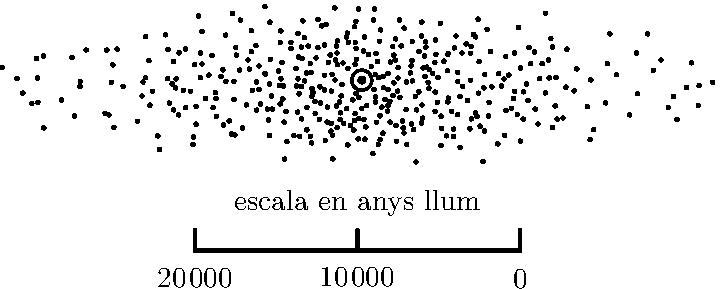
\includegraphics[width=0.7\textwidth]{./images/6-kapteyn}
	\caption{Escala i forma de l'Univers de Kapteyn. El Sol està situat al centre del sistema d'estrelles; l'amplada d'aquest és $\approx 1/5$ del seu radi}
	\label{fig:kapteyn}
\end{figure}

\subsubsection*{Univers de Shapley}
%FIXME: shapley@sec:bio
Harlowe Shapley (1885--1972) va demostrar que aquest univers era erroni. Shapley va utilitzar les estrelles polsants RR Lyrae (la lluminositat variable de les quals les fa destacar) per determinar la distància que ens separa dels cúmuls globulars (que posseeixen RR Lyrae) i va advertir que es distribuïen 2000, aproximadament, amb simetria més o menys esfèrica en torn al centre del disc (no ocupat pel Sol).

Desconeixent la presència de pols al mitjà interestel·lar va sobreestimar les distàncies. No obstant, aquesta descripció és acceptada avui (figura \ref{fig:shapley}).

Els cúmuls globulars se situen bàsicament en l'halo, per això l'extinció per la pols (situada preferentment al disc) afecta poc a la seva lluminositat.

D'aquest anàlisi va resultar que el Sol es troba a uns 25 mil anys llum ($\approx \SI{8}{\kilo\parsec}$) del centre de la Galàxia. Per estudiar el centre de la Galàxia s'ha de recórrer a longituds d'ona típiques de raigs X i raigs gamma. Aquests revelen que esdeveniments altament energètics tenen lloc allà.

El treball de Shapley i l'estudi de la galàxia M31 (Andròmeda) per Walter Baade (1893--1960) va mostrar que la distribució espacial d'estrelles riques en metalls (població I) difereix de la distribució espacial d'estrelles pobres en metalls (població II). Les estrelles al disc són bàsicament de població I; a la protuberància es dóna una barreja d'ambdues poblacions, i en l'halo pràcticament totes són de la població II.

Avui es coneix que la lluminositat del disc és $\approx \SIrange{15}{20}{\Lsun}$, i la de la protuberància és $\approx \SI{5 e9}{\Lsun}$. La massa del disc en estrelles és $\approx \SI{60 e9}{\Msun}$, i la de la protuberància $\approx \SI{20 e9}{\Msun}$. Les estrelles de l'halo contribueixen amb només $\SI{e9}{\Msun}$ a la massa de la Galàxia.
\begin{figure}[ht]
	\centering
	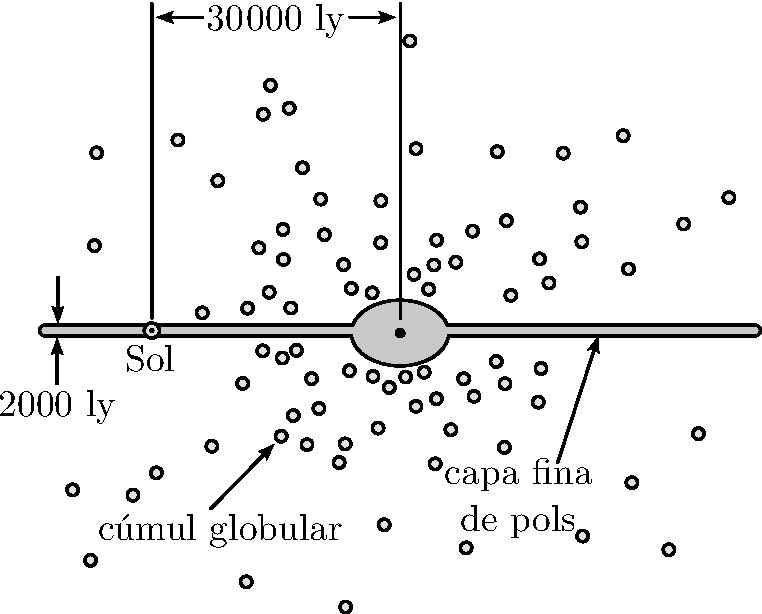
\includegraphics[width=0.55\textwidth]{./images/6-shapley}
	\caption{Visió actual de l'estructura de la Galàxia. Es composa d'un disc prim d'estrelles, gas i pols, una protuberància central, i un halo d'estrelles velles}
	\label{fig:shapley}
\end{figure}

\subsubsection*{Moviment i forma de la galàxia}
El moviment de les estrelles i núvols de gas a la nostra galàxia explica a grans trets la forma d'aquesta.
\begin{figure}[H]
	\centering
	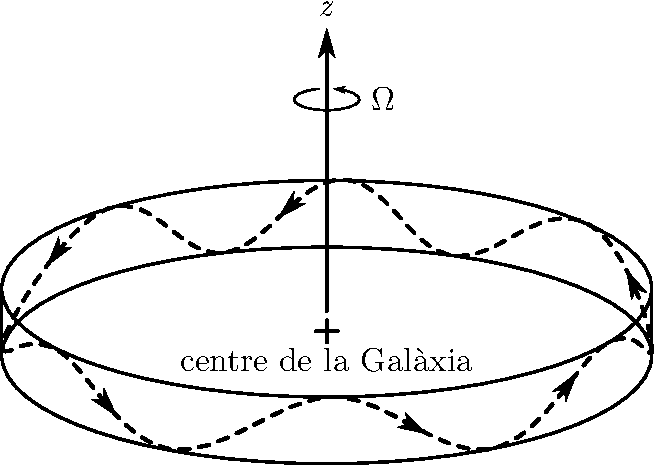
\includegraphics[width=0.5\textwidth]{./images/6-vel-disc}
	\caption{Il·lustració de com la velocitat circular de l'òrbita d'una estrella del disc en ser molt major que la seva velocitat segons l'eix $z$ condueix a que aquestes estrelles donin lloc a una distribució aplanada amb centre al centre de la Galàxia}
	\label{fig:vel-disc}
\end{figure}

El disc està format per estrelles la velocitat de les quals en torn al centre de la Galàxia és molt major que la velocitat del seu moviment erràtic. Això impedeix que col·lapsin a un punt comú i les obliga a romandre al disc (figura \ref{fig:vel-disc}).

La protuberància conté estrelles d'escassa velocitat circular, d'aquesta manera aquestes estrelles formen aproximadament una distribució esfèrica (figura \ref{fig:milky-protuberance}).
\begin{figure}[H]
	\centering
	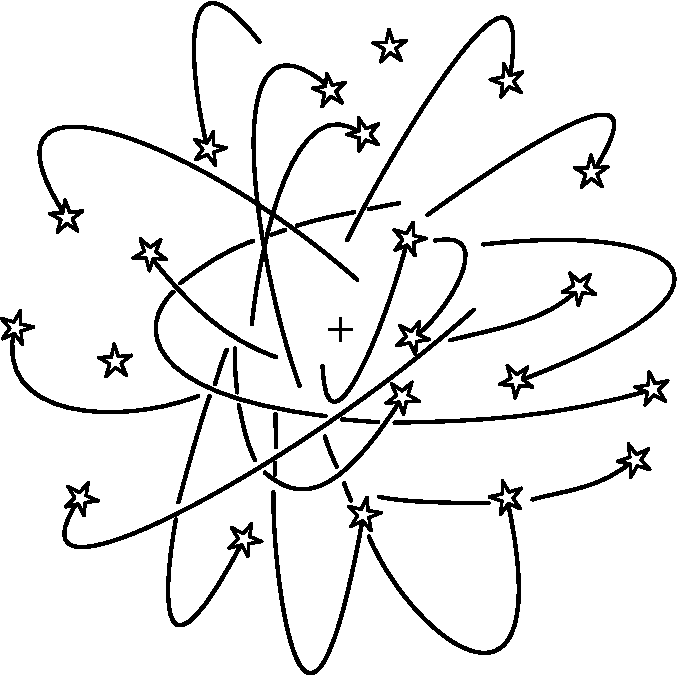
\includegraphics[width=0.5\textwidth]{./images/6-milky-protuberance}
	\caption{La protuberància central està formada per estrelles que no posseeixen una rotació mitjana important. Es mouen en torn al centre $\otimes$ de forma més o menys erràtica donant la impressió (falsa) d'abelles en torn a un rusc. L'equilibri entre el moviment circular i l'atracció gravitatòria cap al centre dóna lloc a la forma esfèrica de la protuberància. La forma exacta d'aquesta no es coneix bé a causa de l'extinció}
	\label{fig:milky-protuberance}
\end{figure}

L'halo està format per estrelles que executen un moviment més o menys harmònic travessant cap a dalt i cap a ball el disc de la Galàxia. La seva component erràtica és clarament major que la de les estrelles del disc i estan menys unides a la Galàxia que les estrelles de la protuberància.

Podria donar-se una transició lenta d'estrelles de la protuberància a l'halo.

%-----------------------------------------------------------------
\subsection{Matèria fosca}
El gruix del disc de la Galàxia al veïnatge del Sol es pot mesurar amb ajuda d'estrelles gegants de tipus espectral K. Aquestes són nombroses i relativament brillants de manera que no són difícils de veure fins i tot a grans distàncies del pla central del disc.

Això, combinat amb mesures de les velocitats erràtiques d'aquestes estrelles, permet deduir la intensitat de la component normal $g_{\perp}$ del camp gravitatori; amb això es pot trobar la massa local necessària per produir aquest camp. A continuació es pot comparar aquesta massa amb la massa observada en forma d'estrelles i núvols de gas.

% FIXME: oort@sec:bio
Per aquest procediment Jan Oort (1895-1965) va descobrir que la massa observada és només la meitat de la requerida per produir aquesta acceleració. Aquesta discrepància és només la primera d'una sèrie detectada en mesures dinàmiques de massa a escala de galàxies i cúmuls de galàxies (el problema de la massa oculta, \textit{missing mass problem}). Se'ns planteja la següent qüestió: existeix potser una massa enorme de matèria no--lluminosa només detectable gràcies a la seva influència gravitatòria?

\subsubsection*{Quocient massa/llum}
Al disc de la Galàxia, al veïnatge del Sol, es té $M/L = 5 \, \Msun/\Lsun$. Aquest valor és també de l'ordre de l'observat en les parts visibles de les galàxies espirals. Això té les següents implicacions:
\begin{enumerate}[(i)]
	\item La massa mitjana de la Galàxia és menys eficaç en produir llum que el Sol. Això es consistent amb el fet que la majoria de les estrelles a la Galàxia són de tipus espectral K febles, o nanes de tipus M, les quals són poc massives (i menys lluminoses que les massives). Hem de concloure, doncs, que la major part de la llum de la Galàxia (excepte en la zona infraroja de l'espectre) procedeix d'un petit nombre d'estrelles massives blaves, i/o de gegants en fase d'evolució avançada. Una fracció important de la massa al disc de la Galàxia està en forma de nanes poc lluminoses i poc massives, i potser en nanes fosques o fins i tot forats negres.
	\item La segona conseqüència es refereix a la producció d'heli. Matèria tan poc eficaç en produir llum no pot haver produït l'heli observat a l'Univers (25\% en massa). El Sol (amb quocient $(M/L)_{\odot} \equiv 1$, per definició) aconsegueix convertir només el 10\% del seu hidrogen en heli en $10^{10}$ anys; de forma que matèria amb $M/L \sim 5$ només convertirà (per processos nuclears) el 2\% del seu hidrogen en heli (en $10^{10}$, aproximadament l'edat de la Galàxia). La major part d'aquest heli es trobaria tancat a l'interior de les estrelles, no incorporant-se a noves generacions d'estrelles; només contribuiria una dècima part a l'heli observat a escales còsmiques.

	Per descomptat, podria ser que els processos nuclears a les estrelles haguessin procedit més ràpidament en temps passats que ara; però els astrònoms creuen que l'heli produït a les estrelles no pot superar en molt 3 cops la producció d'elements pesats (aproximadament 2\% en massa). Així doncs, la major part de l'heli té origen no estel·lar. Molt possiblement va ser produït als primers minuts de l'expansió de l'Univers.
\end{enumerate}

\subsubsection*{Corbes planes de rotació}
Mesures de la línia espectral de $\SI{21}{\cm}$ de l'hidrogen neutre (H I), a causa de l'spin-flip de l'electró, han permès determinar empíricament les corbes de rotació, $v = v(r)$, en més de 100 galàxies espirals.
\begin{figure}[h]
	\centering
	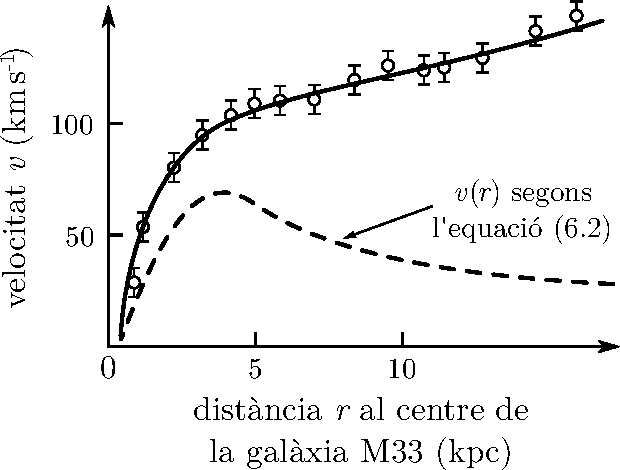
\includegraphics[width=0.5\textwidth]{./images/6-rotation-curve}
	\caption{La corba de rotació de la galàxia espiral nana M33 s'estén molt més enllà de la seva imatge òptica}
	\label{fig:rotation-curve}
\end{figure}

A partir de $\displaystyle m \frac{v^{2}(r)}{r} = G \frac{m M(r)}{r^{2}}$ sobté que la corba de rotació hauria de complir
\begin{align}\label{eq:vel-rotacio}
	v(r) = \sqrt{G \frac{M(r)}{r}}
\end{align}
no obstant els resultats empírics esmentats indiquen una massa molt major que l'observada visualment (matèria fosca). És a dir, la massa de les galàxies segueix creixent molt més enllà tot i que no hi hagi component lluminosa que provoqui aquest augment (figura \ref{fig:rotation-curve}).

Els resultats indiquen que $M/L \approx \SIrange{10}{20}{\Msun/\Lsun}$ a galàxies el·líptiques i espirals; $M/L \approx \SIrange{200}{600}{\Msun/\Lsun}$ a galàxies de baixa lluminositat superficial i a galàxies nanes. En el cas de la galàxia M33 (una galàxia espiral a $\SI{3 e6}{\lightyear}$ de la Via Làctia; [\href{http://apod.nasa.gov/apod/ap030924.html}{APOD~030924}]), es troba que $(M/L)_{Draco} = \SI{440 \pm 240}{\Msun/\Lsun}$.

\subsubsection*{Matèria fosca en cúmuls de galàxies}
Per a cúmuls de galàxies que han assolit l'equilibri dinàmic, el teorema virial
\begin{align}\label{eq:thm-virial}
	K + \frac{1}{2} U = 0
\end{align}
relaciona l'energia cinètica del cúmul $K \approx (3/2) M \ev{v_{r}^{2}}$, on $\ev{v_{r}^{2}}^{1/2}$ és la dispersió de velocitat en la visual, amb l'energia potencial mitjana del cúmul $U \approx - G M^{2}/R$, essent $R$ la mida del cúmul (cúmuls al Catàleg d'Abell solen tenir $R \approx \SI{2.15}{\mega\parsec}$).

La relació \eqref{eq:thm-virial} ens permet determinar l'energia potencial (si la cinètica es coneix amb certa precisió) i d'aquesta deduir la massa gravitatòria del cúmul. El quocient $M/L$ pot arribar a ser tan gran com $\SI{300}{\Msun/\Lsun}$. No obstant això, com que la major part de la massa als cúmuls està en forma de gas calent emissor de raigs X, s'estima que $M/M_{lluminosa} \approx 20$, on $M_{lluminosa}$ és la massa total de matèria lluminosa (incloent-hi estrelles i gas).

Al 1933 Fritz Zwicky (1898--1974) va advertir que les velocitats de les galàxies individuals al Cúmul de Coma eren molt grans, i que aquest cúmul podria romandre lligat gravitacionalment només si la seva massa total excedís substancialment la suma de les masses de les seves galàxies.

\subsubsection*{\textsl{Modified Newton Dynamics} (MOND)}
MOND\footnote{M. Milgrom, \textit{Astrophysical Journal} 270, 365(1983), 384(1983); R. Sanders \& S. McGaugh, \href{http://arxiv.org/abs/astro-ph/0204521}{arXiv:astro-ph/0204521}.} és un intent de substituir la matèria fosca per una altra hipòtesi la qual modificaria la segona llei de Newton, $\va{F} = m \va{a}$, de manera que ara s'escriuria
\begin{align}\label{eq:mond}
	\va{F} = m \mu \qty(\frac{a}{a_{0}}) \va{a}
\end{align}
on $a_{0} \approx \SI{e-8}{\cm \per \square\s}$, i $\displaystyle \mu\qty(\frac{a}{a_{0}}) = \begin{cases} a/a_{0} & \text{si } a \ll a_{0} \\ 1 & \text{si } a \gg a_{0} \end{cases}$.

Si es compara \eqref{eq:mond}, per a $a \ll a_{0}$, amb la fórmula de Newton de l'acceleració gravitatòria, $\va{F} = m \va{g}$, resulta que
\begin{align*}
	a = \sqrt{g a_{0}}
\end{align*}
i ja que l'acceleració centrípeta és $a = v^{2}/r$, se segueix
\begin{align*}
	\frac{v^{4}}{r^{2}} = g a_{0} = G \frac{M}{r^{2}} a_{0}
\end{align*}
de manera que es compleix la relació seüent:
\begin{align}
	v = \qty[G M a_{0}]^{1/4}
\end{align}
és a dir, si l'acceleració és prou baixa (inferior a $\SI{e-8}{\cm \per \square\s}$) la corba de rotació d'un cos aïllat no depèn de la distància $r$ al centre de forces.

Així doncs, MOND no només prediu corbes planes de rotació sinó que implica que l'halo de les galàxies és infinit. Això és un problema per a MOND, ja que hi ha indicis que els halos de les galàxies no s'estenen més enllà de $\SI{0.5}{\mega\parsec}$.

Si bé MOND dóna resultats concordants amb l'observació per a galàxies individuals, no és tan reeixida amb cúmuls de galàxies. En aquests sembla haver una major concentració de massa al centre que predita per MOND. Una altra dificultat amb MOND és la seva resistència a ser inclosa en una teoria de gravitació.

\subsubsection*{Massa de l'halo de la Galàxia}
La massa de l'halo de la Galàxia en forma d'estrelles lluminoses resulta ser d'unes poques centèsimes de la massa del disc. S'ha estès la idea que l'halo contindria un gran nombre de components invisibles o pràcticament invisibles però massives: MACHOs (\textit{Massive Compact Halo Objects}). Aquests podrien ser nanes blanques poc lluminoses, nanes marrons (estrelles que no han aconseguit desencadenar processos nuclears al seu interior), júpiters (planetes de la mida de Júpiter), i forats negres.

Una altra hipòtesi atribueix la massa de l'halo a un oceà de partícules elementals, massives, la interacció de les quals amb la llum i la matèria ordinària (protons, neutrons, electrons) és extraordinàriament lleu: WIMPs (\textit{Weakly Interacting Massive Particles}).

Bé podria ser que ambdós components contribuïssin substancialment a la massa de l'halo. Avui en dia això és una conjectura amb certa base però lluny de ser confirmada.

%-----------------------------------------------------------------
\subsection{Lents gravitacionals}
Segons la relativitat general els raigs de llum pateixen una desviació del seu camí rectilini en passar suficientment prop d'un objecte massiu (en això es va basar el primer test de la relativitat general verificat per Arthur Eddington al 1919 aprofitant un eplipsi solar).
% FIXME: eddington@sec:bio

Si el raig passa a una distància $b$ d'una massa $M$, l'angle de desviació és
\begin{align}\label{eq:alpha-deviation}
	\alpha \approx \frac{4GM}{bc^2} = \frac{2 R_{S}}{b}
\end{align}
on $R_{S} \equiv 2GM/c^2$ es coneix com a \textit{radi de Schwarzschild} de la massa $M$ (pel Sol, $R_{S} \approx \SI{3}{\km}$). La fórmula \eqref{eq:alpha-deviation} és només aproximada; el resultat predit és correcte sempre que $R_{S} \ll b$.
\begin{figure}[H]
	\centering
	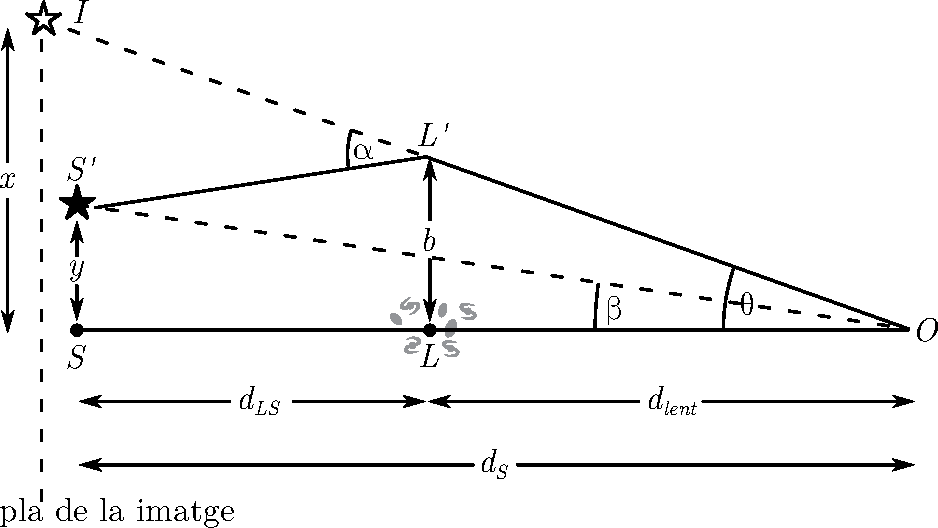
\includegraphics[width=0.75\textwidth]{./images/6-image-gravit}
	\caption{El camp gravitatori d'una massa puntual $M$ (situada a $L$) inclina la llum de l'estrella en $S'$ cap a l'observador. La impressió visual és que l'estrella es troba a $I$}
	\label{fig:image-gravit}
\end{figure}

Mitjançant \eqref{eq:alpha-deviation} es pot calcular la posició de la imatge $I$ si un objecte de massa $M$ s'interposa entre l'estrella $S$ i l'observador $O$ (figura \ref{fig:image-gravit}).

Si no hi hagués lent l'observador veuria l'estrella en $S'$, sota un angle $\beta \approx d_{S}$ (suposant que $y \ll d_{S}$). Ja que la llum s'ha desviat un angle $\alpha$, l'observador veu la imatge sota un angle $\theta \approx x/d_{S}$. Quan $\alpha \ll 1$, se segueix
\begin{align}\label{eq:xyalpha}
	x - y = \alpha d_{LS}
\end{align}
Dividint l'equació \eqref{eq:xyalpha} per $d_{S}$, i tenint en compte l'equació \eqref{eq:alpha-deviation}, suposant que $x \ll d_{S}$, i utilitzant $b \approx \theta d_{L}$, es troba
\begin{align}\label{eq:theta-beta}
	\theta - \beta = \frac{1}{\theta} \frac{4GM}{c^{2}} \frac{d_{LS}}{d_{L} d_{S}} \equiv \frac{\theta_{E}^{2}}{\theta}
\end{align}
on $\theta_{E}$ es coneix com \textit{radi d'Einstein} (tot i que en realitat és un angle).

L'equació \eqref{eq:theta-beta} es pot reescriure com
\begin{align}\label{eq:theta-einstein}
	\theta = \frac{1}{2} \qty[\beta \pm \sqrt{\beta^{2} + 4 \theta_{E}^{2}}]
\end{align}
Aquesta última expressió ens dóna la posició angular de la imatge en termes de l'angle $\beta$ i del radi d'Einstein.
\begin{itemize}
	\item Una estrella exactament darrere la lent ($\beta = 0$) es veurà com un cercle lluminós, al cel, de radi $\theta_{E}$.
	\item Si $\beta > 0$ (la imatge en $\theta_{+}$) apareixerà allunyada de la lent, amb $\theta_{+} > \beta$, fora del radi d'Einstein ($\theta_{+} > \theta_{E}$); aquestes imatges exteriors van ser les observades en torn al Sol eclipsat per la lluna.
	\item La imatge en $\theta_{-}$ és invertida i es troba dins el radi d'Einstein, al lloc oposat de la lent gravitatòria.
\end{itemize}
Tot i que les dues imatges produïdes ($I_{-}$ i $I_{+}$) poden confondre's en una sola (per ser les dues molt properes entre si), podem afirmar que una font lluminosa (estrella, núvol de gas, galàxia, cúmul, quàsar...) està sent afectada per una lent gravitacional (situada entre nosaltres i la font), si apareix més brillant.
\begin{itemize}
	\item Si la lent està en front d'una font extensa, una petita taca de llum al cel es convertirà en dues taques lluminoses en posar la lent entre la font i nosaltres. Les lents gravitacionals no afecten la lluminositat per unitat de superfície, de manera que la lluminositat aparent de cada imatge és proporcional a la seva àrea.
\end{itemize}

Sigui una regió angular $S'$ amb centre en la lent $L$, entre $y$ i $y + \Delta y$ (figura \ref{fig:amplif-lent}).
\begin{figure}[h]
	\centering
	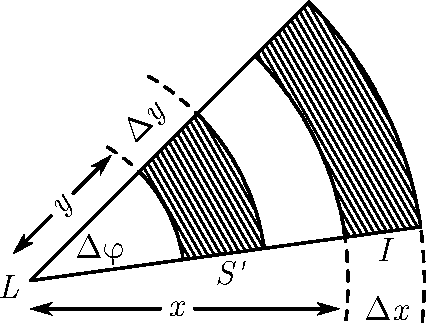
\includegraphics[width=0.35\textwidth]{./images/6-amplif-lent}
	\caption{Amplificació d'una imatge per una lent gravitacional}
	\label{fig:amplif-lent}
\end{figure}

Una imatge $I$ de $S'$ ocupa el mateix angle $\Delta \phi$ que $S'$, però les distàncies relatives al centre $L$ resulten ampliades o contretes:
\begin{align}
	\frac{x}{y} = \frac{\theta}{\beta} \Rightarrow \frac{\Delta x}{\Delta y} = \dv{\theta}{\beta}
\end{align}

En general, una imatge $S'$ més enllà de la lent $L$ resulta més brillant que la taca lluminosa original $S'$ (de no haver intervingut la lent). En canvi, una imatge més propera a l'observador que la lent $L$ resulta menys brillant.

El quocient de les àrees és
\begin{align}
	\frac{A_{imatge}}{A_{font}} = \abs{\frac{\theta}{\beta} \dv{\theta}{\beta}} = \frac{1}{4} \abs{\frac{\beta}{\sqrt{\beta^{2} + 4 \theta_{E}^{2}}} + \frac{\sqrt{\beta^{2} + 4 \theta_{E}^{2}}}{\beta} \pm 2}
\end{align}
de manera que la imatge $\theta_{+}$ és més brillant que la font $S'$, mentre que la imatge $\theta_{-}$ és menys brillant que la font llevat que $\beta < \theta_{E}/ \sqrt{2}$.

Conforme la lent (generalment invisible) es desplaça sobre el fons d'estrelles (pràcticament immòbil) el radi d'Einstein també es desplaça davant una estrella llunyana. Consegüentment veurem augmentar la lluminositat de l'estrella fins assolir un màxim i després decréixer.

Si aconseguim mesurar molts fenòmens de \textit{microlensing} i estudiar el moviment propi de la lent i de la font, la duració mitjana de l'augment en lluminositat ens dóna la massa de les lents gravitatòries. Si la lent consisteix en una estrella binària o en un sistema planetari els components del qual siguin tan propers entre ells que les regions dins dels radis d'Einstein se superposen, les corbes de llum resulten més complicades ja que es formen altres parells d'imatges i apareixen dos o més màxims de llum. En concret, per a una lent de $\SI{0.5}{\Msun}$ a una distància de nosaltres de $\SI{8}{\kilo\parsec}$, i amb una font a dues vegades aquesta distància, es troba que $\theta_{E} \approx \SI{5 e-4}{\arcsecond}$.

\subsubsection*{Objectes compactes massius de l'halo (MACHOs)}
Si suposem que la matèria fosca de l'halo de la Galàxia està constituïda per MACHOs, podrem calcular la probabilitat que una estrella distant sigui pròxima (en l'esfera celeste) a algun MACHO. Com que l'àrea de cada anell d'Einstein ($\pi d_{L}^{2} \theta_{E}^{2}$) és proporcional a la massa de la lent, la suma de totes les àrees només dependrà de la densitat numèrica de MACHOs i no de la massa individual de cadascun d'ells. Donada la massa fosca que es creu que existeix a la Galàxia, qualsevol estrella més enllà de la Galàxia tindrà una probabilitat de $\num{e-6}$ d'estar dins el radi d'Einstein d'algun MACHO. Així doncs, és necessari observar un milió d'estrelles llunyanes per tenir una probabilitat alta de veure alguna d'elles experimentar microlensing.

Una possible objecció a aquest procediment d'estimació observacional de la massa de MACHOs seria que l'augment transitori de lluminositat en una estrela llunyana podria ser degut no a microlensing, sinó a que aquesta estrella és polsant (e.g., una Cefeida). No obstant, en el cas d'estrelles polsants, la variació en lluminositat va acompanyada d'un canvi en temperatura i en color mentre que el microlensing no altera el color, ja que totes les longituds d'ona són afectades per igual pel camp gravitatori de la lent. Per aquesta raó els cercadors de microlensing mesuren la llum de les estrelles fent-les passar per dos filtres de diferents longituds d'ona. Només estrelles la lluminositat de les quals variï en la mateixa proporció en ambdós colors s'acceptaran com a candidats a microlensing.

Cap a l'any 2000 el MACHO Project hauria trobat entre 13 i 17 candidats a microlensing d'estrelles al Gran Núvol de Magalhães. La massa promig d'aquests candidats seria de $\SI{0.5}{\Msun}$ amb una fracció del 20\% de la massa de l'halo (amb un 95\% de confiança si el rang de masses està entre $\SIrange{0.15}{0.9}{\Msun}$, o bé entre $\SIrange{0.08}{0.5}{\Msun}$). Això suggereix que els MACHOs serien nanes blanques, però també podrien ser forats negres formats en transició quark--hadró, poc després del Big Bang.

%-----------------------------------------------------------------
\subsection[Partícules massives d'interacció feble]{Partícules massives d'interacció feble (WIMPs)}
L'estructura de l'Univers a gran escala ens indica que la major part de la matèria no és bariònica, ja que si no les fluctuacions de densitat de matèria en el desacoblament matèria--radiació (300 mil anys després del Big Bang) haurien donat lloc a anisotropies en la radiació de fons de microones molt majors que l'observació ens indica. Això ens diu, no obstant, de quin tipus de matèria no--bariònica es tracta.

L'escenari inicialment proposat, \textit{Hot Dark Matter} (HDM), a començaments dels anys 80, suposava que els WIPMs serien neutrinos, però aviat es va veure la incompatibilitat d'aquesta proposta amb la presència de matèria fosca en galàxies nanes (aquestes no poden retenir a aquests neutrinos donat el seu llarg lliure recorregut mitjà).

A mitjans dels anys 80 es va proposar \textit{Cold Dark Matter} (CDM). Aquest model va estar en voga aproximadament una dècada fins que es va veure la seva incompatibilitat amb les dades més recents d'estructures a gran escala ni amb la proporció de gas en cúmuls de galàxies.

A mitjans dels anys 90 van aparèixer models amb barreja de matèria calenta i matèria freda (CHDM), però aquests tenen dificultats en explicar l'abundància de cúmuls de galàxies. Per una altra banda, la radiació de fons de microones junt amb mesures de la quantitat de matèria present en l'Univers senyala clarament l'existència d'una component d'energia en forma de constant cosmològica (energia del buit) o bé d'un camp escalar.

Entre els diferents candidats a WIMPs en destaquen els neutrinos massius i els axions.

\subsubsection*{Neutrinos massius}
Experiments recents semblen indicar que el neutrino muònic tindria una massa superior a $\SI{0.5}{\eV}$, d'on aquests podrien contribuir amb un 0.5\% a la massa--energia total de l'univers.

Una altra possibilitat és que $m(\nu_{\tau}) \approx m(\nu_{\mu})$, això implicaria que els neutrinos contribuirien fins a un 20\% d'aquesta massa--energia.

Models de partícules elementals més enllà del model estàndard proposen l'existència d'un gran nombre de partícules (no incloses en aquest) de massa fins a $\SI{1}{\tera\eV}$. Tres candidats han estat suggerits:
\begin{itemize}
	\item El sneutrino (spin $= 0$).
	\item El gravitino (spin $= 3/2$).
	\item El neutralino (spin $= 1/2$).
\end{itemize}
D'entre ells, el més afavorit és el neutralino, la massa del qual podria estar entre $30$ i $\SI{60}{\giga\eV}$. De ser així, un continu flux de neutralinos provinents de l'halo de la Galàxia creuaria el nostre planera. D'aquí que hi hagi experiments em marxa orientats a detectar aquest flux.

\subsubsection*{Axions}
Aquestes partícules (també feblement interactives) tindrien masses en el rang de $\SIrange{e-6}{e-2}{\eV}$. Intents de detectar-les han fracassat fins el moment, però la seva base teòrica és tan sòlida que es confia en trobar-les tard o d'hora.

\subsubsection*{Detecció de WIMPs}
Com dèiem més anteriorment, existeixen intents de detectar el suposat flux de WIMPs conforme aquesta travessa la Terra segons aquesta recorre la seva òrbita en torn al Sol. El detector consisteix en $\ch{NaI}$ (iodur sòdic). La interacció d'una partícula WIMP amb un nucli del detector faria que el nucli experimentés un retrocés que es podria mesurar.
\begin{figure}[H]
	\centering
	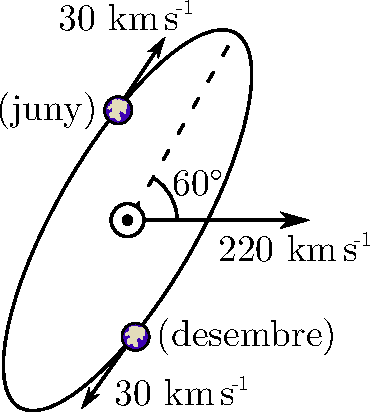
\includegraphics[width=0.25\textwidth]{./images/6-pla-terra-sol}
	\caption{La Terra orbita el Sol. Aquí es mostra la posició del nostre planeta al juny i al desembre}
	\label{fig:pla-terra-sol}
\end{figure}

La Terra orbita el Sol a $\SI{30}{\km\per\s}$ aproximadament, i el Sol orbita la Galàxia a $\SI{220}{\km\per\s}$. El pla de l'òrbita terrestre est 'a inclinat $\SI{60}{\degree}$ respecte al pla del disc de la Galàcia (figura \ref{fig:pla-terra-sol}).

Així és d'esperar que el flux de WIMPs sigui major al juny (quan la velocitat de la Terra i el Sol se sumen) que al desembre (quan es resten). La variació del flux entre ambdós mesos seria del 7\%.

L'experiment DAMA (\textit{Dark Matter Experiment}) sembla mostrar un senyal compatible amb aquestes característiques (figura \ref{fig:dama-results}). No obstant, aquests resultats no han estat corroborats per altres grups, els quals no mostren una variació significativa entre juny i desembre.
\begin{figure}[ht]
	\centering
	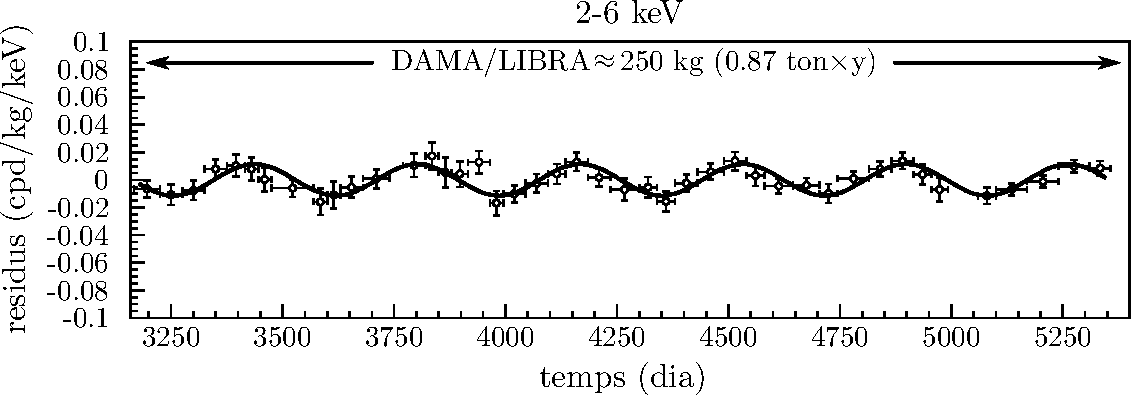
\includegraphics[width=0.9\textwidth]{./images/6-dama-results}
	\caption{Modulació del flux de partícules detectades a l'experiment DAMA en funció del temps}
	\label{fig:dama-results}
\end{figure}

Tanmateix, estan en marxa experiments encaminats a detectar WIMPs per mitjans indirectes. Així, l'anihilació de WIMPs en l'halo produiria un flux de raigs còsmics (integrals per protons i antiprotons). Globus sonda a gran alçada en l'atmosfera han detectat un excés de protons i antiprotons, però podria ser que aquests posseeixin un origen divers com la interacció de raigs còsmics primaris amb protons interestel·lars. L'anihilació de WIMPs podria també donar lloc a una radiació de fons de raigs gamma, amb una intensitat característica d'una ratlla $\gamma$ cap al centre de la Galàxia. El satèl·lit EGRET podria haver ja detectat aquest efecte.

%-----------------------------------------------------------------
%	ROTACIÓ DE LA VIA LÀCTIA
%	!TEX root = ./../main.tex
%-----------------------------------------------------------------
\section{Rotació de la Via Làctia}
%-----------------------------------------------------------------
\subsection{El disc i l'halo de la Via Làctia}
El disc de la Galàxia ha estat objecte d'un estudi més detallat que l'halo.

Al disc les estrelles i els núvols de gas interestel·lar es desplacen en orbites aproximadament circulars en torn al centre de la Galàxia (figura \ref{fig:orbit-star}). La rotació no és uniforme (de sòlid rígid) sinó que les estrelles més properes al centre inverteixen menys temps que les més llunyanes en completar una volta (rotació diferencial $\Omega = \Omega(r)$, figura \ref{fig:star-pattern}).

\begin{figure}[h]
	\centering
	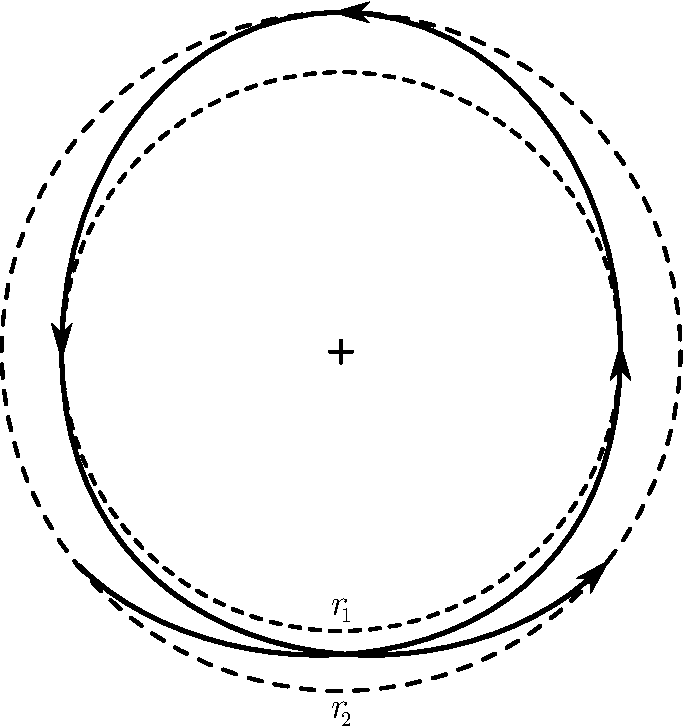
\includegraphics[width=0.55\textwidth]{./images/7-orbit-star}
	\caption{Òrbita d'una estrella projectada sobre el pla del disc. El radi de entre $r_{1}$ i $r_{2}$. El temps invertit en tornar a la distància $r_{2}$ després d'haver partit d'allà és, en general, menor que el temps en completar una volta. L'òrbita no és tancada}
	\label{fig:orbit-star}
\end{figure}

\begin{figure}[h]
	\centering
	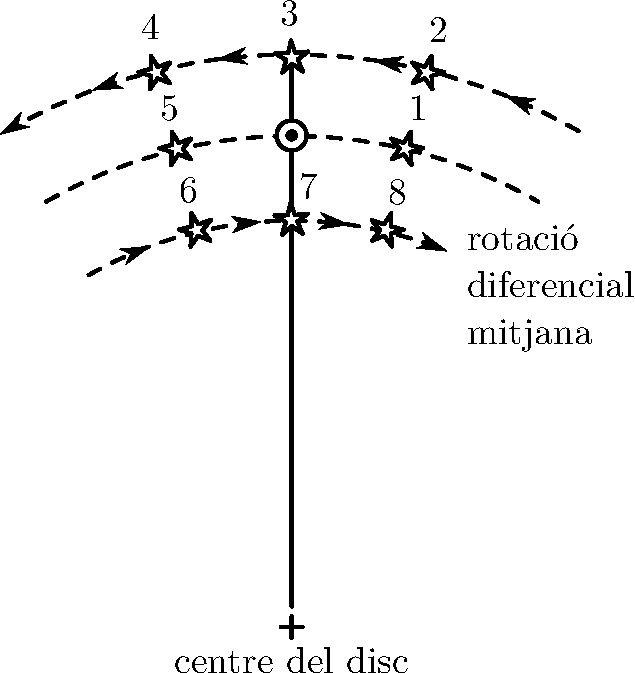
\includegraphics[width=0.45\textwidth]{./images/7-star-pattern}
	\caption{Patró de moviment típic de rotació d'estrelles situades a uns pocs milers d'any llum del Sol ($\odot$)}
	\label{fig:star-pattern}
\end{figure}

La velocitat del Sol en la seva òrbita és $\approx \SI{220}{\km \per\s}$ i el seu període $\approx \SI{200}{\mega\year}$ (si l'edat del Sol és $\approx \SI{5e9}{\year}$, haurà completat la seva òrbita unes 25 vegades).

Les estrelles i núvols de gas propers al Sol viatgen aproximadament a la velocitat d'aquest, de manera que estan gairebé en repòs respecte al Sol. En astronomia es defineix el Sistema de referència estàndard local (\textit{Local Standard of Rest}, LSR) com aquell que segueix el moviment mitjà del material del disc en la velocitat del Sol.

No obstant això, hi ha estrelles a les proximitats del Sol que posseeixen una velocitat notable respecte al LSR. Es dóna el fet curiós que aquestes tenen la seva velocitat cap a una direcció i no cap a l'oposada (figura \ref{fig:asimetria-estrelles}).
\begin{figure}[H]
	\centering
	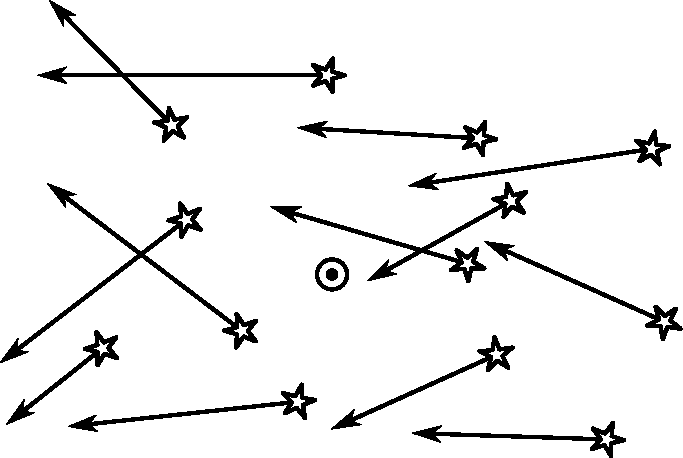
\includegraphics[width=0.5\textwidth]{./images/7-asimetria-estrelles}
	\caption{Asimetria de les estrelles d'\textit{alta velocitat}. Les estrelles que es desplacen a velocitats superiors a $\SI{65}{\km \per\s}$ respecte del sistema estàndard local semblen desplaçar-se exclusivament de dreta a esquerra. No es coneixen estrelles d'alta velocitat que es desplacen al sentit oposat}
	\label{fig:asimetria-estrelles}
\end{figure}

L'explicació d'aquest fenomen és deguda a Lindblad (1895--1965): les estrelles d'alta velocitat posseeixen en realitat baixa velocitat rotacional i gran velocitat no rotacional. El Sol (i altres estrelles) giren ràpidament deixant-les al darrere per la qual cosa les d'\textit{alta velocitat} semblen fluir en sentit oposat. Nosaltres tenim a considerar al Sol en repòs, però si l'observem des del centre de la Galàxia, comprovaríem que les estrelles d'\textit{alta velocitat} posseeixen en realitat un moviment més lent que el Sol.

La figura \ref{fig:star-pattern} mostra que, en mitjana, les estrelles situades entre el Sol i el centre del disc inverteixen menys temps que aquest en completar una òrbita en torn al centre del disc, mentre que les situades més lluny al centre que el Sol inverteixen més temps. Aquesta rotació diferencial recolza la tesi que el Sol no és al centre de la Galàxia.

Mesures observacionals permeten determinar el cisallament (\textit{shear}) de la rotació diferencial en l'entorn del Sol i la \textit{vorticitat}. Aquestes magnituds venen donades a través de les constants $A$ i $B$ de Oort definides per
\begin{align}
	A = - \frac{r}{2} \dv{\Omega}{r} \qc B = -\frac{1}{2r} \dv{\qty(r^{2}\Omega)}{r},
\end{align}
de manera que
\begin{align}
	\Omega = A - B
\end{align}

Observacionalment es troba que
\begin{align*}
	A = \SI{0.005}{\km \per\s \per\lightyear} \qc \sqrt{1 - A/B} = 1.6
\end{align*}
La constant $A$ mesura el cisallament i s'obté de mesures de les velocitats radials al veïnatge solar. A la vegada, mesures de moviments propis mitjans ens donen la constant $B$ (vorticitat). Com la figura \ref{fig:vel-erratic} indica, en les proximitats del Sol, les estrelles tenen velocitats erràtiques predominantment orientades cap al centre de la Galàxia. Conegudes $A$ i $B$ es determina $\Omega$, i el període $2\pi/\Omega$ (aproximadament 220 milions d'anys per a estrelles properes al Sol). Això, juntament amb la distància del Sol al centre del disc ($\approx \SI{25}{\giga\lightyear}$), ens permet determinar la velocitat orbital del Sol en aproximadament $\SI{220}{\km\per\s}$.

\begin{figure}[h]
	\centering
	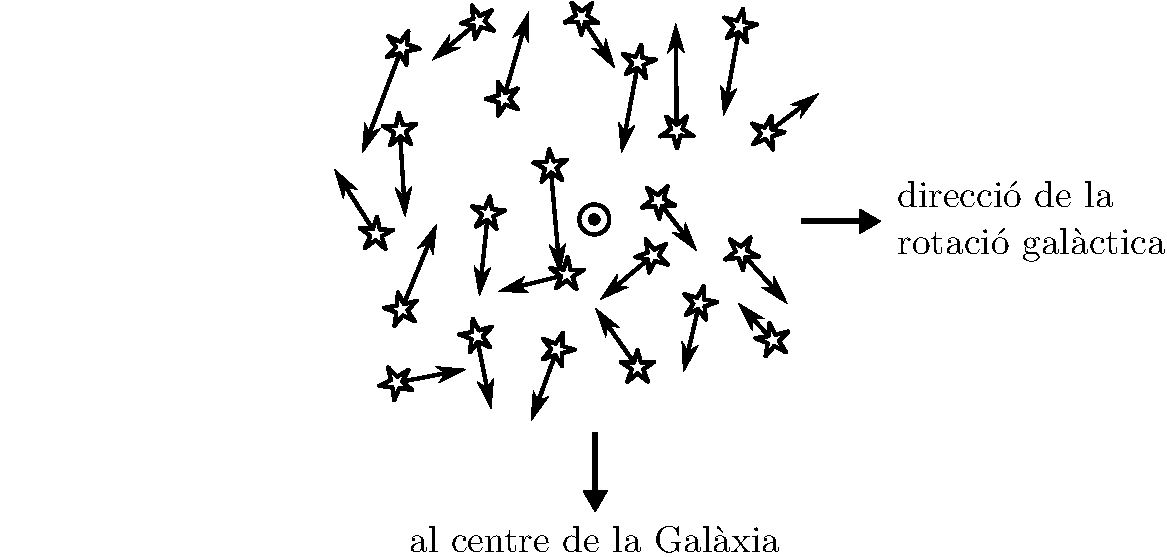
\includegraphics[width=0.8\textwidth]{./images/7-vel-erratic}
	\caption{Les velocitats erràtiques de les estrelles al veïnatge del Sol tendeixen a ser majors cap al centre de la Galàxia que en la direcció de rotació. Aquesta asimetria en la dispersió de velocitats també mostra que la Galàxia no gira com sòlid rígid}
	\label{fig:vel-erratic}
\end{figure}

Tanmateix, es pot estimar la massa de la Galàxia interior a l'òrbita solar com $M(r) = v^{2} r / G \approx \SI{e11}{\Msun} > M_{lluminosa}$.

Malgrat l'enorme nombre d'estrelles a la Galàxia, una col·lisió és altament improbable (excepte, és clar, en sistemes lligats: estrelles binàries, cúmuls d'estrelles; o al centre de la Via Làctia).

\subsubsection*{Coordenades galàctiques}
Per descriure el moviment de les estrelles al disc convé introduir dos sistemes de coordenades diferents (figura \ref{fig:coordenades-galactiques}):
\begin{itemize}
	\item Un sistema de coordenades cilíndriques $(r, \theta, z)$ amb origen al centre del disc (útil per a la descripció teòrica).
	\item Un sistema $(R,l,b)$ centrat al Sol (útil per a la descripció observacional), on $R$, és la distància al Sol, $l$ la longitud, i $b$ la latitud.
\end{itemize}

\begin{figure}[h]
	\centering
	\includegraphics[width=0.9\textwidth]{./images/7-coordenades-galactiques}
	\caption{Coordenades galàctiques. Els astrònoms acostumen a presentar les seves observacions al pla galàctic com si el contempléssim de dalt cap a baix. Llavors, als dibuixos observacionals el sentit de rotació de la Galàxia en torn a l'eix $Z$ és el sentit horari}
	\label{fig:coordenades-galactiques}
\end{figure}

\subsubsection*{Òrbites estel·lars al disc}
A ordre zero, el camp gravitatori al disc resulta estacionari (independent del temps) i amb simetria axial. Per tant, dins d'aquesta aproximació, l'energia per unitat de massa i el moment angular per unitat de massa són constants del moviment.
\begin{align*}
	E = \frac{1}{2} \qty(v_{r}^{2} + v_{\theta}^{2} + v_{z}^{2}) + V(r,z) \approx cte \qc J = r v_{\theta} \approx cte
\end{align*}

Tenint això en compte, les òrbites al disc no són exactament circulars: superimposat al moviment circular es dóna un altre segons l'el·lpse centrada al cercle i en sentit retrògrad; és a dir, es tracta d'un \textit{epicicle} (figura \ref{fig:galaxy-epicycle}) tal que les freqüències angulars d'ambdós moviments ($\kappa$ i $\Omega$) difereixen en general. Per una altra part, la freqüència del moviment alllarg de l'eix $z$ és major que $\kappa$ i $\Omega$.
\begin{figure}[h]
	\centering
	\includegraphics[width=0.5\textwidth]{./images/7-galaxy-epicycle}
	\caption{Epicicle. Si l'òrbita és lleugerament no circular, aquesta pot entendre's com formada per la superposició d'un moviment circular de velocitat angular constant $\Omega$, i un moviment retrògrad, el·líptic de freqüència $\kappa$ amb centre al cercle}
	\label{fig:galaxy-epicycle}
\end{figure}

Per conèixer l'estructura de la Galàxia a gran escala (i d'això dedir la seva distribució de massa) hem de determinar la posició i velocitat de rotació d'objectes molt llunyans al Sol. En aquesta tasca ens servim de la longitud d'ona de $\SI{21}{\cm}$ de l'hidrogen atòmic.

Suposem un radiotelescopi localitzat al Sol i apuntant en la direcció de la longitud galàctica $l$ amb $b = 0$. A la figura \ref{fig:patro-rotacio} s'adverteix que el núvol de gas 2 és d'especial interès, ja que només hi ha un punt tangent (o punt subcentral).

A causa de la rotació diferencial, el núvol 2 (més proper que els altres de la figura \ref{fig:patro-rotacio} al centre de la Galàxia) es mou amb major velocitat que els altres núvols respecte a nosaltres. Els núvols 1 i 3 s'allunyen més lentament, el núvol 4 apareix amb velocitat zero ja que es troba a igual distància que el Sol al centre de la Galàxia, i el núvol 5 (extern a l'òrbita del Sol) s'aproxima a nosaltres (posseeix velocitat radial negativa). El cas del núvol 2 és molt especial ja que
\begin{align*}
	r = r_{\odot} \sin l
\end{align*}
on $r_{\odot}$ és la distància del Sol al centre de la Galàxia ($\approx \SI{8.5}{\kilo\parsec}$).
\begin{figure}[H]
	\centering
	\includegraphics[width=0.6\textwidth]{./images/7-patro-rotacio}
	\caption{Patró de rotació diferencial a gran escala per a un observador al sistema local de referència. Cal notar que els núvols 1 i 3 posseeixen igual velocitat al llarg de la visual (velocitat radial), i el núvol 2 té la velocitat radial positiva major; el núvol 4 apareix en repòs, i el 5 posseeix una velocitat negativa}
	\label{fig:patro-rotacio}
\end{figure}

\begin{figure}[H]
	\centering
	\includegraphics[width=0.47\textwidth]{./images/7-perfil-21cm}
	\caption{Perfil esquemàtic de la intensitat de la línia de $\SI{21}{\cm}$ neutre font a la velocitat radial. La màxima velocitat es dóna per al núvol 2 (al punt de tangència)}
	\label{fig:perfil-21cm}
\end{figure}

Per tant, per trobar les velocitats i posicions d'objectes en òrbites interiors al Sol, l'estratègia és apuntar el radiotelescopi a diferents longituds $l$; així s'obté la velocitat radial $v(r)$ per a diferents distàncies radials (del punt de tangència) al centre de la Via Làctia. El resultat es mostra a la figura \ref{fig:gal-corba-rotacio1}, corba de rotació de la Galàxia.
\begin{figure}[H]
	\centering
	\includegraphics[width=0.51\textwidth]{./images/7-gal-corba-rotacio1}
	\caption{Corba de rotació de la Galàxia obtinguda mitjançant observacions de $\lambda = \SI{21}{\cm}$ de l'àtom d'hidrogen per a núvols de gas interiors al cercle solar}
	\label{fig:gal-corba-rotacio1}
\end{figure}

Com que més enllà del cercle solar no hi ha punts tangents, aquest mètode només serveix per a objectes que es mouen en òrbites interiors a aquest cercle.

La corba de rotació de la Galàxia per a objectes que es mouen en òrbites externes a la solar s'obté mesurant per mitjans òptics la distància a objectes la velocitat radial de les quals es desitja determinar.
\begin{figure}[H]
	\centering
	\includegraphics[width=0.51\textwidth]{./images/7-gal-corba-rotacio2}
	\caption{Corba de rotació de la Galàxia estesa més enllà del cercle solar per mitjans fotomètrics d'estrelles OB i emissió de \ch{CO} de núvols moleculars gegants}
	\label{fig:gal-corba-rotacio2}
\end{figure}

Se sol recórrer a complexes H II (hidrogen ionitzat) gegants als límits del disc, ja que experimenten poc enfosquiment degut a la pols interestel·lar i les seves distàncies es poden trobar fotomètricament (tot i que no amb gran exactitud) estudiant les propietats òptiques de les estrelles que exciten aquests núvols. Núvols moleculars gegants solen acompanyar als complexes H II, i les velocitats radials d'aquests núvols moleculars poden trobar-se a partir de la seva emissió de \ch{CO} (monòxid de carboni). Aquest mètode permet estendre la corba de rotació de la Galàxia fins a gairebé $\SI{2}{r_{\odot}}$. La corba completa es mostra a la figura \ref{fig:gal-corba-rotacio2}. És obvi que la rotació de la Galàxia és diferencial.

\subsubsection*{Espessor de la capa de gas}
El mètode del punt tangent (al qual li correspon la màxima velocitat al llarg de la visual, per a una longitud $l$ fixa) se suposa vàlid fins i tot encara si la coordenada angular $b$ és lleugerament diferent de zero. Mitjançant l'estudi del descens en intensitat de la línia $\SI{21}{\cm}$ d'hidrogen atòmic conforme el radiotelescopi escombra diferents valors de $b$ (latitud galàctica) tot mantenint $l$ (longitud), els astrònoms mesuren l'amplada efectiva dels punts de tangència.

Es troba que la capa d'hidrogen presenta una amplada pràcticament constant d'uns $\SI{700}{\lightyear}$ ($\approx \SI{214}{\parsec}$) per a tots els radis interiors a l'òrbita solar.

Mesures anàlogues s'han portat a terme per a mesuraments de \ch{CO} per les distribucions de gas molecular, trobant que aquest posseeix una amplada de $\SI{300}{\lightyear}$ ($\approx \SI{92}{\parsec}$). Com que el diàmetre del cercle solar és d'aproximadament $\SI{5 e4}{\lightyear}$, veiem que les capes de gas i pols a la Via Làctia són proporcionalment tan primes com un naip.

Es coneix que la capa d'hidrogen atòmic s'estén molt més enllà de l'òrbita solar, mostrant, a més a més, una duplicitat en la seva perifèria (figura \ref{fig:disc-perfil}). Aquest efecte, també observat en altres galàxies, podria atribuir-se al fet que els núvols de Magalhães hagin passat recentment molt a prop de la Galàxia, produint efectes de marea.
\begin{figure}[h]
	\centering
	\includegraphics[width=0.65\textwidth]{./images/7-disc-perfil}
	\caption{Vista de perfil (esquemàtica) del disc gasós de la Galàxia mostrant el seu eixamplament més enllà de l'òrbita solar i la seva duplicitat en la perifèria}
	\label{fig:disc-perfil}
\end{figure}

\subsubsection*{Estructura esquemàtica de la Via Làctia}
La figura \ref{fig:galaxy-scheme} mostra una vista esquemàtica de la Galàxia. La protuberància central posseeix un radi d'uns pocs kiloparsecs. El Sol es troba al disc prim a uns $\SI{8}{\kilo\parsec}$ del nucli, que allotja, sembla ser, un forat negre de massa $\approx \SI{4 e6}{\Msun}$ (que experimenta un augment aproximat de $\SI{7e-10}{\Msun \per\year}$).

\begin{figure}[h]
	\centering
	\includegraphics[width=0.8\textwidth]{./images/7-galaxy-scheme}
	\caption{Vista esquemàtica de la Via Làctia}
	\label{fig:galaxy-scheme}
\end{figure}

El \textit{disc prim} conté el 95\% de les estrelles del disc i totes les estrelles massives joves. La seva alçada d'escala (la distància que ens hem de desplaçar perpendicularment al disc perquè la seva densitat caigui en un factor $e$) està entre $\SIrange{300}{400}{\parsec}$. La resta d'estrelles forma el \textit{disc gruixut} amb una alçada d'escala entre $\SIrange{1000}{1500}{\parsec}$. Les estrelles del disc gruixut són més velles que les del disc prim i són més pobres en elements químics pesats. El gas i la pols jeuen en una capa encara més prima que la de les estrelles. Es creu que la matèria fosca se situa per totes parts i també a l'halo de la Galàxia, per aquesta raó és a vegades anomenat l'\textit{halo fosc} (\textit{dark halo}).

%-----------------------------------------------------------------
\subsection{Estructura espiral}
Estudis de la posició i velocitat de núvols de gas hidrogen neutre i núvols moleculars suggereixen que el disc de la Galàxia presenta una estructura espiral de 3 braços semblant a la galàxia NGC 4622 [\href{http://apod.nasa.gov/apod/ap040221.html}{APOD~040221}]. Als braços espirals es dóna una fort concentració de gas i al seu si té lloc la gènesi de noves estrelles. Efectivament, els discs de les galàxies espirals posseeixen un color blau més destacat que ;a resta del disc i les emissions de \ch{H_{$\alpha$}} revelen l'existència de gas calent i ionitzat envoltant estrelles joves massives. Com que estrelles suficientment calents per emetre fotons ultraviolats capaços d'ionitzar àtoms d'hidrogen viuen només 10 milions d'anys, els braços espirals deuen ser llocs on contínuament es formin estrelles. A coordenades galàctiques $(r,l)$ la forma espiral d'una galàxia de $m$ braços es pot representar mitjançant
\begin{align}\label{eq:gal-spirals}
	\cos\qty{m\qty[l + f(r,t)]} = 1
\end{align}
on $f(r,t)$ mesura quant estretament (o no) estan units entre si els braços: si $\abs{\pdv*{f}{r}}$ és gran, els braços estan pegats els uns als altres; si $\abs{\pdv*{f}{r}}$ és petit, llavors estan més oberts. L'angle $i$ entre les tangents al braç espiral i al cercle de radi $r$ que el talla en aquest punt (figura \ref{fig:gal-spiral}) ve donat per
\begin{align}\label{eq:gal-spiral-i}
	\cot i = \abs{r \pdv{l}{r}} = \abs{r \pdv{f}{r}}
\end{align}

\begin{figure}[ht]
	\centering
	\includegraphics[width=0.5\textwidth]{./images/7-gal-spiral}
	\caption{En un disc que roti en sentit contrari a les agulles del rellotge i en què la velocitat angular $\Omega(r)$ decreixi amb $r$, estrelles inicialment situades al llarg d'un radi es disposarien més tard en una espiral estreta seguint el moviment darrere}
	\label{fig:gal-spiral}
\end{figure}

Es creu que els braços espirals corresponen a ones de densitat; de no ser així, la rotació diferencial de la Galàxia donaria en poc temps que els braços quedessin estrets en un rínxol (cosa que no s'observa). Per veure això amb cert detall suposem que inicialment les estrelles estiguin disposades al llarg d'una línia radial amb $l = l_{0}$ (figura \ref{fig:gal-spiral}). Cada estrella descriu la seva òrbita amb velocitat $v(r)$ (recordem que la velocitat angular és $\Omega(r) = v(r)/r$), de manera que després d'un temps $t$ aquestes estrelles jeuen al llarg de l'espiral
\begin{align*}
	l = l_{0} + \Omega(r) t
\end{align*}
Combinant aquesta expressió amb l'equació \eqref{eq:gal-spirals} se segueix
\begin{align*}
	m \qty[l_{0} + \Omega(r) t + f(r,t)] = 0
\end{align*}
o, equivalentment,
\begin{align}
	f(r,t) = -l_{0} - \Omega(r) t
\end{align}

Com que, en general, $\Omega(r)$ decreix amb $r$, per a $\Omega(r) > 0$ s'infereix que $f(r,t)$ augmenta conforme ens movem al llarg del braç cap a valors de $r$ creixents, així que $l$ ha de disminuir (perquè se segueixi complint l'equació \eqref{eq:gal-spirals}). Tenim, doncs, una \textit{trailing spiral} ja que l'extrem del braç apunta en el sentit oposat al gir; i conforme passa el temps, l'espiral es fa més i més estreta.

Al veïnatge del Sol $v(r)$ ($\approx \SI{220}{\km \per\s}$) és aproximadament constant i $r \approx \SI{8}{\kilo\parsec}$, l'angle $i$ (donat per l'equació \eqref{eq:gal-spiral-i}) s'estrenyeria d'acord amb
\begin{align*}
	\cot i = r \abs{\dv{\Omega(r)}{t}} t \approx \frac{220}{8} \frac{t}{\SI{1}{\giga\year}} \Leftrightarrow i \approx \SI{2}{\degree} \times \qty(\frac{\SI{1}{\giga\year}}{t})
\end{align*}
Després de $\num{e9}$ anys, l'espiral resultaria molt més estreta que les espirals observades a galàxies anàlogues a la Via Làctia. Qualsevol patró inicial patiria un estrenyiment semblant.

El fenomen d'estructura espiral de galàxies és molt complex i probablement siguin varis mecanismes els responsables d'aquest. Un cop el núvol de gas ha produït les primeres estrelles, ones de xoc de les supernoves (corresponents a l'explosió d'estrelles de vida curta) comprimeixen el gas que les envolta. Això pot ocasionar el naixement de més estrelles, així que la producció d'aquestes es propaga a través del gas. A continuació, la rotació diferencial arrossega el núvol a un segment del braç espiral \textit{endarrerit}. Per quan aquest fregament hagi estat fortament estirat, el gas s'haurà esgotat, les estrelles calentes s'hauran apagat i la regió retorna al disc.

Aquest model d'\textit{autopropagació de formació d'estrelles} serà eficaç només si el ritme de naixement d'estrelles pot auto-regular-se de tal manera que no mori mai ni faci cremar tot el disc esgotant el seu gas. Aquest mecanisme pot explicar l'estructura espiral de la galàxia M33, però no probablement la del sistema M100 [\href{http://apod.nasa.gov/apod/ap010203.html}{APOD~010203}], on els braços espirals giren més de $\SI{180}{\degree}$.

Un paràmetre clau en la formació de l'estructura espiral és el paràmetre d'estabilitat de Toomre:
\begin{align}
	Q = \frac{\kappa \sigma_{r}}{3.36 G \Sigma}
\end{align}
on $\kappa$ és la freqüència de l'epicicle (figura \ref{fig:galaxy-epicycle}), $\sigma_{r}$ és la dispersió de velocitats estel·lars al llarg de la visual, i $\Sigma$ és la densitat superficial del disc.

Simulacions mitjançant ordinador mostren que una estructura espiral només apareixerà si $Q \gtrsim 1.2$. Conforme l'estructura espiral es desenvolupa, la mida dels epicicles en les òrbites estel·lars augmenta i amb això $Q$. Així doncs, no s'espera observar una estructura espiral amb $Q < 1$ (figura \ref{fig:gal-simulation}).
\begin{figure}[H]
	\centering
	\includegraphics[width=\textwidth]{./images/7-gal-simulation}
	\caption{Simulació per ordinador mostrant com un disc de $\num{50000}$ partícules que s'atreuen mútuament per gravetat desenvolupa primer un patró espiral de dos braços, i després una barra al centre. El bulb galàctic i l'halo fosc són representats per una força cap a dins. La simulació correspon a $\SI{2.65}{\giga\year}$ si el radi del disc és de $\SI{16}{\kilo\parsec}$ i la massa de la galàxia és de $\SI{2 e11}{\Msun}$; el disc comença amb $Q = 1$}
	\label{fig:gal-simulation}
\end{figure}

Al veïnatge solar, i per a estrelles d'edat semblant al Sol ($\approx \SI{5 e9}{\year}$) es té $\sigma_{r} \approx \SI{30}{\km \per\s}$, $\Sigma \approx \SI{50}{\Msun \per\square\parsec}$, $\kappa \approx \SI{36}{\km \per\s \per\kilo\parsec}$, de manera que $Q \approx 1.4$, valor compatible amb l'estructura espiral.

%-----------------------------------------------------------------
%	AGRUPACIONS DE GALÀXIES
%	!TEX root = ./../main.tex
%-----------------------------------------------------------------
\section{Agrupacions de galàxies}\label{sec:galaxies}
\subsection{Classificació de les galàxies}
Les galàxies solen classificar-se atenent al seu aspecte en la longitud d'ona del visible.

El tipus més abundant de galàxia és el de nana poc lluminosa; les galàxies grans i les gegants emeten una enorme quantitat de llum.

L'existència de galàxies (més enllà de la Via Làctia) va ser establida als anys 20. Abans d'això, apareixien als catàlegs com a «nebuloses», sistemes lluminosos, suposadament dins els confins de la Galàxia. En les imatges captades pels telescopis les nebuloses apareixien borroses i per tant es creia que eren mancants d'estrelles.
\begin{figure}[h]
	\centering
	\includegraphics[width=0.8\textwidth]{./images/8-hubble-scheme}
	\caption{Esquema original de Hubble amb certes modificacions}
	\label{fig:hubble-scheme}
\end{figure}

Hubble, amb l'ajut del telescopi del \textit{Mount Wilson Observatory} (MWO), va trobar estrelles variables a la «nebulosa» M31 (Andròmeda) [\href{http://apod.nasa.gov/apod/ap130626.html}{APOD~130626}], i va advertir que el ritme de variació de la llum seguia el mateix patró que les Cefeides de la Via Làctia. Sota la hipòtesi que eren estrelles del mateix tipus, va aplicar l'equació $F = L/ (4\pi d^2)$ tot trobant $d \gtrsim \SI{300}{\kilo\parsec}$ com a distància a Andròmeda; de manera que aquesta havia de ser una galàxia i no un sistema interior a la Via Làctia. Avui dia se sap que la distància a Andròmeda és aproximadament $\SI{800}{\kilo\parsec}$.

Hubble va establir a \textit{The Realm of the Nebulae} (1936) un esquema de classificació de les galàxies (figura \ref{fig:hubble-scheme}). En dit esquema hi ha tres tipus de galàxies (el·líptiques, lenticulars, i espirals) més un quart tipus (irregulars) per aquelles que no s'ajusten a cap dels tipus interiors.

%-------------------------------
\subsubsection*{Galàxies el·líptiques (E)}
Són arrodonides sense característiques especials (ni braços espirals ni franges de pols). Normalment manquen de núvols freds de gas per la qual cosa posseeixen no poques estrelles blaves joves. Un estudi detallat revela que les el·líptiques gegants posseeixen una estructura diferent de les petites i poc lluminoses. N'hi ha amb un disc dins el cos el·líptic.

Les el·líptiques predominen en cúmuls de moltes galàxies i les el·líptiques més grans (galàxies CD) solen trobar-se en la zona més densa d'aquests cúmuls. Les galàxies CD consten d'un nucli el·líptic rodejat d'una enorme i difusa embolcall que pot assolir centenars de kiloparsecs. Aquests sistemes arriben a ser fins a 100 cops més lluminosos que la Via Làctia.

Les el·líptiques de mida mitjana i gegants posseeixen una lluminositat varies vegades la de la Galàxia, i mides de l'ordre de desenes de kiloparsecs. Les seves estrelles segueixen un moviment en aparença poc organitzat i les seves òrbites en torn al centre de la galàxia estan orientades erràticament. En el·líptiques menys massives i menys lluminoses les estrelles tenen un moviment més ordenat i menys erràtic.

Les el·líptiques molt poc lluminoses ($\sim 1/10$ de la Via Làctia) solen ser de dos tipus:
\begin{enumerate}[(i)]
	\item Galàxies compactes, com el sistema M32 [\href{http://apod.nasa.gov/apod/ap960106.html}{APOD~960106}].
	\item Galàxies nanes difuses (dE) [\href{http://apod.nasa.gov/apod/ap001023.html}{APOD~001023}], i les encara menys lluminoses nanes esferoïdals (dSph) [\href{http://apod.nasa.gov/apod/ap990122.html}{APOD~990122}]. Aquestes últimes són a penes visibles a les plaques fotogràfiques.
\end{enumerate}

Les galàxies tipus dE i les dSph no mostren gairebé moviment de rotació.

%-------------------------------
\subsubsection*{Galàxies lenticulars (S0)}
Posseeixen un disc rotatori a més d'un cos central el·líptic, però aquest manca de braços espirals o de grans franges de pols. Poden considerar-se com un tipus intermedi entre el·líptiques i espirals. Són semblants a les el·líptiques en el fet que solen trobar-se a regions molt poblades. S'assemblen a les espirals en la presència del disc que gira ràpidament. N'és un exemple la galàxia NGC 2787 [\href{http://apod.nasa.gov/apod/ap020408.html}{APOD~020408}].

%-------------------------------
\subsubsection*{Galàxies espirals (S)}
Posseeixen braços espirals brillants en què destaca la llum blava d'estrelles joves. Els braços queden delineats per grups per grups d'estrelles O i B calents, i per núvols de gas i pols a partir de les quals es formen aquestes estrelles.

Aproximadament la meitat de les espirals i lenticulars posseeixen una barra central. Els sistemes SB0, SBA, \dots, SBd formen una seqüència paral·lela a les galàxies sense barra.

Al llarg de la seqüència Sa, \dots, Sd la protuberància central es fa menys important amb respecte al disc (que gira ràpidament) i els braços s'obren més i més; i la proporció de gas i estrelles joves al disc augmenta. La Via Làctia és una Sc i potser una Sbc. Andròmeda (M31) és una Sb. En mitjana, galàxies Sc i Sd són menys lluminoses que les Sa i Sb, però algunes Sc són més brillants que una Sa típica.

Cap al final de les seqüències de galàxies espirals, Sd i SBd, els braços apareixen menys ordenats i discontinus (a trossos). Les Sm i SBm són les espirals de Magalhães (el prototip de les quals és LMC, el Gran Núvol de Magalhães [\href{http://apod.nasa.gov/apod/ap130528.html}{APOD~130528}]). En aquestes, l'espiral es redueix a un únic i ample braç. Conforme la lluminositat de la galàxia decreix, la velocitat de rotació del disc disminueix. Les galàxies menys brillants són menys massives. El Gran Núvol de Magalhães gira només a $\SI{80}{\km \per\s}$, un terç de la velocitat de rotació de la Via Làctia.

El moviment estel·lar erràtic també disminueix en les galàxies petites, però, tot i així, el moviment rotacional ordenat forma una part menys important de la seva energia total.

%-------------------------------
\subsubsection*{Galàxies irregulars (Irr)}
Hubble va situar en aquest grup totes aquelles galàxies que no s'ajusten a cap dels tres tipus anteriors.

Avui dia s'utilitza el nom d'\textit{irregular} només per a galàxies blaves, petites mancants de braços espirals o de qualsevol altra estructura organitzada. Les nanes irregulars es diferencien de les nanes esferoïdals en el fet que posseeixen fas i estrelles joves blaves. És possible que les nanes esferoïdals no siguin més que nanes irregulars que han esgotat o perdut gairebé tot el seu gas.

\subsubsection*{Catàlegs de galàxies}\label{sec:catalogues}
\begin{itemize}
	\item Charles Messier (1784) va catalogar 109 objectes, entre ells Andròmeda (M31).
	% FIXME: messier@sec:bio
	\item \textit{New General Catalogue} (John Dreyer, 1888, amb addicions al 1895 i al 1908), basat fonamentalment en el treball de William Herschel, conté més de 7000 objectes lluminosos com ara cúmuls d'estrelles, núvols gasosos, i galàxies. Andròmeda és NGC~224.
	% FIXME: herschel@sec:bio
	\item El catàleg de la NASA \textit{Extragalactic Database} és accessible via web: \url{https://ned.ipac.caltech.edu/}.
	\item \textit{David Dunlap Observatory Catalogue}, conegut com a DDO o \textit{A Catalogue of Dwarf Galaxies}, és un catàleg de galàxies nanes que va ser publicat al 1959 (amb addicions al 1966) per Sidney van den Bergh (1929).
\end{itemize}

%-----------------------------------------------------------------
\subsection{Fotometria galàctica}
Les galàxies no apareixen com punts de llum (cas de les estrelles) sinó com objectes extensos i borrosos sobre el fons fosc del cel nocturn (l'observació òptica de les galàxies requereix un cel sense lluna o lluna nova). La turbulència de l'atmosfera ocasiona que les galàxies apareguin borroses, i que els telescopis terrestres no puguin distingit detalls per baix de $\SI{1/3}{\arcsecond}$.

Interessa conèixer quanta llum és emesa a diferents longituds d'ona per les diferents regions de la galàxia sota observació. Per fer-ho es defineix la lluminositat superficial.

\begin{defi}[Lluminositat superficial, $I(\va{x})$]
	Es defineix la lluminositat superficial, $I(\va{x})$, com la quantitat de llum per segon d'arc quadrat sobre el cel en un punt $\va{x}$ de la imatge.

	Sigui un petit quadrat de costat $D$ a la imatge d'una galàxia que es troba a una distància $d$, de manera que aquest quadrat subtendeix un angle $\alpha = D/d$ al cel, llavors
	\begin{align}\label{eq:llum-sup}
		I(\va{x}) \equiv \frac{F}{\alpha^{2}} = \frac{L}{4\pi D^{2}}
	\end{align}
	on $L$ és la lluminositat del quadrat en qüestió.

	En un principi $I(\va{x})$ no depèn de la distància a la galàxia, no obstant, si la distància és molt gran, l'efecte d'expansió de l'Univers intervé a través del desplaçament $z$ cal al vermell.
\end{defi}

Els contorns $I(\va{x}) = cte$ s'anomenen \textit{isofotos}. L'equació \eqref{eq:llum-sup} mostra que la posició d'un isofoto en una galàxia és independent d'aquest observador.

La lluminositat superficial sol ser mesurada en una banda determinada de longitud d'ona. Es centres de galàxies solen assolir només $I_{B}(\va{x}) \approx \SI{18}{^{\prime\prime-2}}$ i $I_{R}(\va{x}) \approx \SI{16}{^{\prime\prime-2}}$. Els disc estel·lars són encara menys brillants.

Ja que les galàxies manquen de fronteres ben definides per estimar la seva mida, aquesta es mesura dins un isofoto donat. Freqüentment s'agafa l'isofoto de magnitud $m = 25$ a la banda $B$ (blava), denotat com $R_{25}$. Aquest és aproximadament l'1\% de la lluminositat del cel nocturn típic. Una altra possibilitat de mesura de la mida d'una galàxia és el \textit{radi de Holmberg}, corresponent a $I_{B}(\va{x}) = \SI{26.5}{^{\prime\prime-2}}$.

Per determinar la lluminositat d'una galàxia completa es mesura l'augment de lluminositat conforme augmenta la distància des del centre de la galàxia cap a l'exterior, tot extrapolant aquest resultat per trobar el total.

La lluminositat superficial d'una galàxia espiral decau amb la distància $r$ al seu centre al llarg del semieix major segons la llei de de Vaucouleurs:
\begin{align}\label{eq:vancouleurs}
	I(r) = I_{0} \exp[-\qty(r/r_{0})^{1/4}]
\end{align}
Aquesta llei també regeix la variació de la lluminositat en la protuberància central.

La llum al disc d'una galàxia espiral varia sinusoïdalment amb l'angle azimutal. Si aquesta llum és integrada sobre un cercle per obviar l'estructura espiral, la distribució de llum al disc segueix la llei empírica
\begin{align}
	I(r) = I_{0} \exp[-r/r_{0}]
\end{align}

Mentre que $r_{0}$ varia notablement d'una galàxia espiral a una altra, $I_{0}$ varia poc, sent el seu valor de l'ordre de $\SI{2 e4}{\Lsun \per\square\lightyear}$. No obstant, s'ha trobat que la constància de $I_{0}$ no regeix per a galàxies nanes, i probablement tampoc per a les gegants.

Hi ha moltes més galàxies poc lluminoses que grans i brillants. La figura \ref{fig:nombre-galaxies} mostra el nombre de galàxies observades en funció de la seva lluminositat $L$ segons mesures de l'\textit{Observatorio de Las Campanas} (Xile). La línia contínua correspon a la funció de Schechter:
\begin{align}\label{eq:schechter}
	\Phi (L) \Delta L = n_{\star} \qty(\frac{L}{L_{\star}}) \exp[-\frac{L}{L_{\star}}] \frac{\Delta L}{L_{\star}}
\end{align}
on $L_{\star} \approx \SI{2 e10}{\Lsun}$, més o menys la lluminositat de la Via Làctia.

\begin{figure}[h]
	\centering
	\includegraphics[width=0.6\textwidth]{./images/8-nombre-galaxies}
	\caption{Nombre de galàxies $\Phi (M)$ per a $\SI{10}{\cubic\mega\parsec}$ front a la lluminositat. La línia contínua segueix la llei de Schechter. La línia discontínua és $\Phi(M) \times L/L_{\star}$. Aquí $h \approx 0.75$ és el factor reduït de Hubble, $\alpha = -0.7$ i $n_{\star} - \SI{0.019}{\cubic\planck \per\cubic\mega\parsec}$}
	\label{fig:nombre-galaxies}
\end{figure}

A la figura \ref{fig:nombre-galaxies} s'adverteix que el nombre de galàxies en cada interval de lluminositat $\Delta L$ és quasi constant per a $L < L_{\star}$, i cau ràpidament per a $L > L_{\star}$.

La fórmula de Schechter diu que el nombre total de galàxies $\int_{0}^{\infty} \Phi (L) \dd{L}$ divergeix per a $L \to 0$. No obstant, la línia discontínua ens diu que la major part de la llum ve de les galàxies de lluminositat en torn a $L_{\star}$. La integració de la funció de Schechter ens dóna la lluminositat total:
\begin{align}
	 \int_{0}^{\infty} \Phi (L) \dd{L} = n_{\star} \Gamma (\alpha + 2) \approx \SI{1.4 e8}{\planck \Lsun \per\cubic\mega\parsec}
\end{align}

%-----------------------------------------------------------------
\subsection{El Grup Local}
El grup al que pertany la Via Làctia (Grup Local) conté, aproximadament, tres dotzenes de galàxies en una esfera de $\SI{1}{\mega\parsec}$ de radi amb centre entre la Galàxia i Andròmeda (vegeu la taula \ref{tab:grup-local}).

Els tres membres més destacats (M31, la Via Làctia, i M33) són galàxies espirals. M31 (Andròmeda) posseeix una lluminositat 1.5 vegades la de la Via Làctia; M33 només 0.2 vegades. El 90\% de la lluminositat, en el rang de longituds d'ona del visible, del Grup Local és degut a aquestes tres. L'única galàxia el·líptica del grup és M32, una galàxia satèl·lit d'Andròmeda. Les restants són nanes o irregulars.

Les distàncies que figuren a la taula \ref{tab:grup-local} s'han obtingut triant Cefeides individuals dins de cada galàxia, mesurant la seva magnitud aparent, i estimant la seva vertadera lluminositat mitjançant la relació període--lluminositat \eqref{eq:cepheid} de Cefeides variables.

Així doncs, les distàncies a les deu galàxies més brillants s'ha aconseguit establir amb un error de només el 10\%. No obstant, a galàxies menys lluminoses hi ha menys estrelles per triar i l'error és major. En el cas d'algunes galàxies nanes, l'error és superior al 50\%.

Moltes galàxies nanes són satèl·lits de la Via Làctia o d'Andròmeda. Altres, en canvi, no estan lligades a cap galàxia en particular (només al Grup Local). És certament probable que existeixin encara més galàxies al Grup Local, ja que podria haver galàxies nanes ocultes per la pols del disc de la Via Làctia.
\\

L'atracció gravitatòria dins el Grup Local ha superat l'expansió global de l'Univers. Així, en molts casos, les galàxies dins el grup s'aproximen les unes a les altres en comptes d'allunyar-se. En concret, la Via Làctia i Andròmeda s'aproximen entre si a una velocitat de l'ordre de $\SI{120}{\km\per\s}$. Les velocitats radials de les altres galàxies jeuen, en general, en un interval de $\SI{60}{\km \per\s}$ respecte al moviment conjunt de la Galàxia Andròmeda. Podem dir que les galàxies del nostre grup local manquen de velocitat suficient per abandonar el grup; les seves velocitats són inferiors a la d'escapament.

Les galàxies, en un radi d'aproximadament $\SI{30}{\mega\parsec}$ en torn a la Via Làctia, se situen en un pla, el \textit{pla supergalàctic}, més o menys perpendicular al disc de la Galàxia en la direcció $l = \SI{140}{\degree}$ i $l = \SI{320}{\degree}$.

El cúmul de galàxies més proper al Grup Local és el Cúmul de Virgo [\href{http://apod.nasa.gov/apod/ap150407.html}{APOD~150407}], aproximadament a $\SI{15}{\mega\parsec}$ de nosaltres. És un cúmul relativament irregular en què es dóna una zona central densa constituïda per galàxies velles rodejada per una zona extensa formada principalment per galàxies espirals. El Grup Local està caient cap al Cúmul de Virgo. Aquest pertany al \textit{Supercúmul Local}, tot ocupant el seu centre.

El Cúmul de Coma [\href{http://apod.nasa.gov/apod/ap080616.html}{APOD~080616}], a uns $\SI{90}{\mega\parsec}$ de la Via Làctia i aquell al qual cau el Cúmul de Virgo, forma part d'un altre supercúmul. La mida d'un supercúmul sol estar entre $\SIrange{10}{20}{\mega\parsec}$. No obstant això, a aquestes escales no és possible parlar pròpiament de sistemes individuals. Més encertat és considerar els sistemes de galàxies com una xarxa contínua on els grans cúmuls estan connectats entre si mitjançant petits cúmuls que fan de pont.

\begin{table}[ht]
	\small
	\centering
		\begin{tabular}{l l c c r r}
		\toprule
		Galàxia & Tipus & $d$ ($\si{\kilo\parsec}$) & $L_{v}$ ($\SI{e7}{\Lsun}$) & $l$ ($\si{\deg}$) & $b$ ($\si{\deg}$) \\
		\midrule
		M31 (NGC 224) $\circ$     & Sb  & \num{770} & \num{2700} & \num{121} &  \num{-22} \\
		Via Làctia $\bullet$      & Sbc & \num{8} & \num{1500} & \num{0} &  \num{0} \\
		M33 (NGC 598)             & Sb  & \num{850} & \num{550} & \num{134} &  \num{-31} \\
		Large MC $\bullet$        & SBm & \num{49} & \num{170} & \num{280} &  \num{-33} \\
		NGC 205 $\circ$           & dE  & \num{850} & \num{40} & \num{121} &  \num{-21} \\
		%
		Small MC $\bullet$        & Irr & \num{58} & \num{34} & \num{303} &  \num{-44} \\
		M32 (NGC 221) $\circ$     & E2  & \num{750} & \num{30} & \num{121} &  \num{-22} \\
		NGC 6822                  & Irr & \num{490} & \num{30} & \num{25} &  \num{-18} \\
		IC 10                     & Irr & \num{820} & \num{20} & \num{119} &  \num{-3} \\
		NGC 147 $\circ$           & dE  & \num{760} & \num{12} & \num{120} &  \num{-14} \\
		%
		NGC 185 $\circ$           & dE   & \num{600} & \num{10} & \num{121} &  \num{-15} \\
		IC 1613 (DDO 8)           & dIrr & \num{715} & \num{10} & \num{130} &  \num{-61} \\
		Pegasus (DDO 216)         & dIrr & \num{760} & \num{8} & \num{95} &  \num{-44} \\
		WLM (DDO 221)             & dIrr & \num{970} & \num{4} & \num{76} &  \num{-74} \\
		Leo A (DDO 69)            & dIrr & \num{690} & \num{2} & \num{197} &  \num{52} \\
		%
		Fornax $\bullet$          & dSph & \num{120} & \num{1.4} & \num{237} &  \num{-66} \\
		Sagittarius $\bullet$     & dSph & \num{25} & \num{1} & \num{6} &  \num{-14} \\
		And I $\circ$             & dSph & \num{770} & \num{0.5} & \num{122} &  \num{-25} \\
		Leo I (DDO 74) $\bullet$  & dSph & \num{270} & \num{0.5} & \num{226} &  \num{49} \\
		And VII/Cas dSph $\circ$  & dSph & \num{760} & \num{0.5} & \num{110} &  \num{-10} \\
		%
		And II $\circ$            & dSph & \num{590} & \num{0.3} & \num{129} &  \num{-29} \\
		And VI/Peg dSph $\circ$   & dSph & \num{830} & \num{0.3} & \num{106} &  \num{-36} \\
		Aquarius (DDO 210)        & dIrr & \num{950} & \num{0.2} & \num{34} &  \num{-31} \\
		Sculptor $\bullet$        & dSph & \num{72} & \num{0.14} & \num{288} &  \num{-83} \\
		Sagittarius DIG           & dIrr & \num{800} & \num{0.1} & \num{21} &  \num{-16} \\
		%
		And III $\circ$           & dSph      & \num{770} & \num{0.1} & \num{119} &  \num{-26} \\
		Phoenix                   & dIrr/dSph & \num{420} & \num{0.08} & \num{272} &  \num{-69} \\
		Cetus                     & dSph      & \num{775} & \num{0.08} & \num{101} &  \num{-73} \\
		LGS3 (Pisces)             & dIrr/dSph & \num{810} & \num{0.06} & \num{127} &  \num{-41} \\
		Leo II (DDO 93) $\bullet$ & dSph      & \num{207} & \num{0.06} & \num{220} &  \num{67} \\
		%
		Tucana                    & dSph & \num{870} & \num{0.05} & \num{323} &  \num{-47} \\
		Sextans $\bullet$         & dSph & \num{83} & \num{0.04} & \num{244} &  \num{42} \\
		Carina $\bullet$          & dSph & \num{100} & \num{0.03} & \num{260} &  \num{-22} \\
		And V $\circ$             & dSph & \num{810} & \num{0.03} & \num{126} &  \num{-15} \\
		Ursa Minor $\bullet$      & dSph & \num{64} & \num{0.02} & \num{105} &  \num{45} \\
		Draco (DDO 216) $\bullet$ & dSph & \num{72} & \num{0.02} & \num{86} &  \num{35} \\
		\bottomrule
	\end{tabular}
	\caption{Galàxies del Grup Local. La Via Làctia i els seus satèl·lits estan indicats amb $\bullet$, Andròmeda (M31) i les seves companyes estan indicades amb $\circ$}
	\label{tab:grup-local}
\end{table}

%-----------------------------------------------------------------
%	DISTRIBUCIÓ DE LES GALÀXIES A GRAN ESCALA
%	!TEX root = ./../main.tex
%-----------------------------------------------------------------
\section{Distribució de les galàxies a gran escala}
\subsection{Forma i edat de l'Univers}
\subsubsection*{La paradoxa d'Olbers (1829)}
Suposem un Univers infinit amb les estrelles distribuïdes uniformement. Considerem el cel nocturn. El nombre $N$ d'estrelles en una esfera de radi $r$ centrada a la Terra serà
\begin{align}
	N \propto r^{2}
\end{align}
i el flux de radiació rebut a la Terra de cadascuna d'aquestes esferes serà
\begin{align}
	F \propto \frac{1}{r^{2}}
\end{align}
Llavors, $NF = cte$ serà el flux rebut a la Terra a causa de les estrelles en aquesta superfície. En un univers infinit hi hauria un nombre il·limitat d'aquestes superfícies, de manera que el flux total divergiria i el cel nocturn hauria de ser al menys tan lluminós com el diürn.

Aquesta paradoxa ens indica que es compleix alguna de les següents hipòtesis:
\begin{itemize}
	\item L'Univers no és infinit en extensió.
	\item L'Univers no s'expandeix, per la qual cosa la llum de les estrelles pateixen un desplaçament cap al roig proporcionant-nos menys llum que en un Univers estàtic.
	\item Les estrelles no han existit sempre.
\end{itemize}
En definitiva, l'idea d'un Univers infinit i etern (és a dir, sense començament) no és sostenible.

\subsubsection*{L'expansió de l'Univers}
L'any 1923 Edwin Hubble va demostrar que la galàxia M31 (Andròmeda) es troba més enllà de la Galàxia.

Les galàxies es presenten aïllades (\textit{field galaxies}) o formant part d'un grup que pot ser petit (grup, varies dotzenes, com és el cas del nostre Grup Local), mitjanes (cúmuls, centenars), o molt grans (supercúmuls, possiblement una agrupació de cúmuls).

Les estructures de major mida observades fins a la data són aproximadament de $\SI{100}{\mega\parsec}$, clarament més petites que el volum d'espai explorat ($\sim$ varis milers de $\si{\mega\parsec}$).

La distribució de galàxies se sol estudiar cantant el nombre $N(m)$ de galàxies més brillants que la d'una magnitud $m$ donada (figura \ref{fig:N-magnitud}).

Si les galàxies estiguessin distribuïdes uniformement, tindríem que
\begin{align}
	N(<m) \sim 10^{0.6 m}
\end{align}

Efectivament, suposem que totes les galàxies posseeixen la mateixa magnitud absoluta $M$. La distància, en parsecs, ve donada per
\begin{align*}
	d = 10^{(m - M +5 )/5} \si{\parsec}
\end{align*}

\begin{figure}[H]
	\centering
	\includegraphics[width=0.4\textwidth]{./images/9-N-magnitud}
	\caption{El canvi de pendent a partir de la magnitud 18 pot entendre's a causa de l'expansió de l'Univers}
	\label{fig:N-magnitud}
\end{figure}

Així, per poder veure una estrella de lluminositat $m$ o major (menor $m$) s'ha de trobar dins d'una esfera de radi $d$ centrada a la Terra.

Com que la distribució de galàxies se suposa uniforme, el seu nombre $N$ serà proporcional a $d^{3}$, és a dir,
\begin{align}
	N \propto d^{3} \propto 10^{0.6 m}
\end{align}
Aquest resultat és independent de la magnitud absoluta $M$, llavors és també vàlid quan les magnituds absolutes difereixen entre si.

L'estudi realitzat per Hubble (1934) basat en aproximadament $\num{44000}$ galàxies indicava una distribució homogènia i isòtropa il·limitada (sense fronteres). Estudis anàlegs sobre radiofonts extragalàctiques mostren que les radiofonts eren més brillants o més nombroses al passat. Això indica que l'Univers no és estàtic sinó que evoluciona.

\subsubsection*{La llei de Hubble (1929)}
Les línies espectrals de les galàxies llunyanes es troben desplaçades cap al roig (figura \ref{fig:galaxies-spectra}) tant més com més distant es troba la galàxia en qüestió:
\begin{align}
	\Delta \lambda \equiv \lambda_{obs} - \lambda_{em} \approx \frac{H_{0}}{c} r \lambda_{em}
\end{align}
on $H_{0}$ és la constant de Hubble ($\approx \SI{70}{\km \per\s \per\mega\parsec}$) i $r$ la distància a la galàxia.
\begin{figure}[H]
	\centering
	\includegraphics[width=0.7\textwidth]{./images/9-galaxies-spectra}
	\caption{Fotografies i espectres (redshifts) de galàxies localitzades a diferents cúmuls; relació entre el redshitf i la distància
per a galàxies remotes}
	\label{fig:galaxies-spectra}
\end{figure}

En termes del redshift, la llei de Hubble s'escriu
\begin{align}\label{eq:hubble-law}
	z = \frac{H_{0}}{c} r
\end{align}
Si el desplaçament és cap al roig és degut a l'efecte Doppler, llavors $z = v/c$, aleshores
\begin{align}
	v = H_{0} r
\end{align}
Aquest fet se sol interpretat com l'expansió de l'Univers (figura \ref{fig:hubble-diagram}).
\begin{figure}[h]
	\centering
	\includegraphics[width=0.55\textwidth]{./images/9-hubble-diagram}
	\caption{Diagrama de Hubble mostrant la correlació entre el redshift (eix $y$) i un indicador de distància basat en cúmuls el·líptics de primera classe (eix $x$)}
	\label{fig:hubble-diagram}
\end{figure}

Hubble va determinar que $H_{0} \approx \SI{500}{\km \per\s \per\mega\parsec} \approx \SI{1/2}{\per\giga\year}$, molt major que el valor acceptat avui dia.

Hubble només va prendre 18 galàxies, les distàncies a les quals va estimar a partir de la seva magnitud aparent $m$ de les seves estrelles més brillants. No obstant, les galàxies més distants utilitzades pertanyen al Cúmul de Virgo, amb velocitat radial de $\SI{e3}{\km \per\s}$, no molt major que l'arrel quadrada de la velocitat quadràtica mitjana de la velocitat peculiar de les galàxies.

Si aquest valor fos cert, ens trobaríem amb el fet que l'Univers seria més jove ($\approx \SI{2}{\giga\year}$) que la Terra ($\approx \SI{4.5}{\giga\year}$).

Amb el pas dels anys s'han aconseguit determinacions més precises de $H_{0}$. Aparentment
\begin{align*}
	60 \lesssim H_{0} \lesssim \SI{85}{\km \per\s \per\mega\parsec}
\end{align*}
essent $\SI{70}{\km \per\s \per\mega\parsec}$ el valor més acceptat avui. L'edat de l'univers (determinada per diferents mètodes) sembla ser compatible amb $\SI{13.7}{\giga\year}$.

Tenint en compte la relació
\begin{align*}
	m = M + 5 \log(\frac{r}{\SI{10}{\parsec}})
\end{align*}
per a un conjunt d'\textit{espelmes estàndards} (\textit{standard candles}, galàxies i/o supernoves de magnitud absoluta propera a un valor mitjà $M_{0}$), es veu que
\begin{align}
	m = M_{0} + 5 \log(\frac{cz}{H_{0} \times \SI{10}{\parsec}}) = 5 \log z + cte
\end{align}
on la constant depèn de $H_{0}$ i $M_{0}$.

El valor de la constant de Hubble és difícil de determinar per diferents raons:
\begin{enumerate}[(i)]
	\item Incertesa en les distàncies a les galàxies llunyanes.
	\item Velocitat peculiar de les galàxies.
\end{enumerate}
Possiblement el nostre Grup Local posseeixi una velocitat no menyspreable ($\approx \SI{250}{\km \per\s}$) cap al Cúmul de Virgo. Com que aquest s'utilitza freqüentment per determinar $H_{0}$, si aquesta velocitat peculiar no es té en compte, es comet un error notable.

La llei de Hubble pot donar la falsa impressió que la nostra Galàxia ocupa el centre de l'Univers. Aquesta conclusió és falsa, com el lector pot raonar fàcilment a partir de la figura \ref{fig:gal-no-centre}.
\begin{figure}[h]
	\centering
	\includegraphics[width=0.8\textwidth]{./images/9-gal-no-centre}
	\caption{Il·lustració del repòs relatiu de la Via Làctia a l'Univers, que dóna la sensació que aquesta sigui el centre de l'Univers}
\label{fig:gal-no-centre}
\end{figure}

\subsubsection*{L'edat de l'Univers}
L'edat de la Terra, determinada a través de l'abundància relativa d'elements radioactius a la seva escorça és de $\approx \SI{4.5}{\giga\year}$. L'edat del sistema solar, estimada mitjançant l'abundància de \ch{^{87}Rb} relativa a la de \ch{^{87}Sr} en meteorits (\ch{^{87}Rb -> ^{87}Sr}, $\tau_{1/2} = \SI{4.99 e10}{\year}$) ve a ser aproximadament $\SIrange[range-units = repeat]{4.5}{5.0}{\giga\year}$. L'edat de les roques lunars se situa entre $\SIrange[range-units = repeat]{4.5}{4.6}{\giga\year}$. L'edat dels cúmuls globulars (a l'halo de la Galàxia) es troba en l'interval $\SIrange[range-units = repeat]{11.5}{16}{\giga\year}$.

L'edat estimada de l'Univers, $t_{0}$ (és a dir, el temps transcorregut des de l'inici de la seva expansió), segons resultats extrets de les dades del satèl·lit WMAP és
\begin{align*}
	t_{0} \approx \SI{13.7}{\giga\year}
\end{align*}
Aquest resultat és compatible amb $H_{0}^{-1} \approx \SI{14}{\giga\year}$, tal com prediuen els models cosmològics en voga.

\subsubsection*{L'abundància relativa d'heli}
El nucli d'heli (\ch{^{4}_{2}He}) és el més abundant a l'Univers després del d'hidrogen (\ch{^{1}_{1}H}); aproximadament 75\% d'hidrogen i 25\% d'heli en massa.

La major part de l'heli no és d'origen estel·lar sinó còsmic, produït en els primers instants de l'expansió de l'Univers a partir dels protons i neutrons lliures existents en aquella època.

La cadena de reaccions nuclears conduents a l'heli és complicada, no obstant el procés més significatiu és el següent:
\begin{align*}
\begin{cases}
	\ch{$p$ + $m$ -> D + $\gamma$} \\
	\ch{D + D -> ^{3}He + $n$ -> ^{3}H + $p$} \\
	\ch{^{3}He + D -> ^{4}He + $n$}
\end{cases}
\end{align*}
on $\ch{D} \equiv \ch{^{2}_{1}H}$ és el que anomenem deuteri o hidrogen pesant.

Aquest procés resulta efectiu un cop la temperatura del gas de fotons cau per sota de $T_{D} \approx \SI{8 e8}{\K}$, ja que quan $T > T_{D}$ el fas de fotons dissocia el deuteri (l'energia d'enllaç del deuteri és $B_{D} = m_{p} + m_{n} - m_{D} - \SI{1.71}{\MeV}$) de la següent manera:
\begin{align*}
	\ch{$\gamma$ + D -> $p$ + $n$}
\end{align*}

El fet que només el 25\% (en massa) dels nuclis siguin d'heli (i no pràcticament el 100\%) indica que l'Univers va passar per una fase de molt elevada temperatura caracteritzada per un gas de fotons amb temperatura superior a $T_{D}$.

La nucleosíntesi primordial (diferent de l'estel·lar) va finalitzar als 15 o 16 minuts d'iniciada l'expansió.

\subsubsection*{La radiació de fons de microones}
El gas de fotons es va anar refredant amb l'expansió de l'Univers:
\begin{align}
	T \propto \frac{1}{a}
\end{align}
on $a$ és el factor d'escala.

% FIXME: gamow@sec:bio
Com que el cas està en equilibri amb si mateix, ha de presentar una distribució de cos negre. L'existència d'aquest bany de radiació tèrmica va ser predita pels components de la nucleosíntesi primordial (George Gamow, Ralph Alpher, i Robert Herman) cap a finals dels anys 40 i descoberta fortuïtament pels astrofísics Arno Penxias i Robert Wilson al 1965.

La temperatura de la radiació de fons és avui de
\begin{align*}
	T_{0} \approx \SI{2.726}{\K}
\end{align*}
i, llevat de desviacions molt lleugeres, efectivament posseeix espectre de Planck (de cos negre).

Aquestes desviacions no són superiors a la centmil·lèsima part:
\begin{align*}
	\ev{\frac{\Delta T}{T_{0}}} \approx \num{e-5}
\end{align*}
Sense aquestes petites desviacions respecte al valor mitjà, $T_{0}$, l'existència de les galàxies no es podria entendre dins del model cosmològic estàndard (el més amplament acceptat).

Durant, aproximadament, els primers 380 mil anys de l'inici de l'expansió, la matèria (protons, electrons, i nuclis d'hidrogen, principalment) interaccionava amb la radiació (fotons) fonamentalment mitjançant
\begin{align*}
	\ch{$p$ + $e^{-}$ <-> H + $\gamma$}
\end{align*}
tot mantenint l'equilibri tèrmic entre matèria i radiació. Quan la temperatura va descendir per sota de $\approx \SI{3000}{\K}$, aquesta reacció ja no va ser efectiva per mantenir l'equilibri i els fotons es van poder propagar lliurement. Aquests fotons constitueixen la radiació de fons de microones (figura \ref{fig:dispersio-cmbr}).
\begin{figure}[h]
	\centering
	\includegraphics[width=0.85\textwidth]{./images/9-dispersio-cmbr}
	\caption{Diagrama simplificat de la superfície de l'última dispersió}
	\label{fig:dispersio-cmbr}
\end{figure}

%-----------------------------------------------------------------
\subsection{El model cosmològic estàndard}
\subsubsection*{El principi cosmològic}
D'igual manera que la Terra no ocupa una posició especial al sistema solar, ni aquest a la Galàxia, ni aquesta dins del nostre Grup Local, podem donar un pas més i formular la següent hipòtesi:
\begin{quote}
	\textit{«A una escala prou gran, l'aspecte que l'Univers presenta és independent del punt d'observació.»}
\end{quote}

Com podem veure a la figura \ref{fig:principi-cosmologic}, al petit cercle $A$ entorn l'observador $O$, la distribució de galàxies no és representativa de la densitat de galàxies a gran escala. Sí, en canvi, al cercle $B$.

Aquesta hipòtesi, a la pràctica, no és verificable (i podria no ser correcta) ja que avui només podem observar l'Univers des de la nostra galàxia.

El principi cosmològic no afirma que l'Univers sigui homogeni i isòtrop. Aquesta afirmació segueix d'advertir que és isòtrop\footnote{Cal notar que si un espai presenta isotropia en torn a cada punt, llavors és també homogeni.} en torn a la nostra galàxia (com l'observació mostra, específicament l'alt grau d'isotropia, $\sim \num{e-5}$, de la radiació de fons de microones), i d'aplicar el principi cosmològic.

Aquest principi comporta una gran simplificació a l'hora d'estudiar l'Univers des del punt de vista matemàtic.
\begin{figure}[h]
	\centering
	\includegraphics[width=0.7\textwidth]{./images/9-principi-cosmologic}
	\caption{El principi cosmològic. Per a l'observador ($O$) el cercle petit ($A$) no representa una distribució uniforme a gran escala. Al cercle gran ($B$) aquesta distribució ja és uniforme en mitjana}
	\label{fig:principi-cosmologic}
\end{figure}

\subsubsection*{Geometria de l'Univers: factor d'escala}
Si l'Univers és efectivament isòtrop (a gran escala) en torn a la Galàxia i acceptem el principi cosmològic, la distància entre si, de l'espai--temps ve donada per l'element de línia
\begin{align}\label{eq:flrw-metric}
	\dd{s^{2}} = - c^{2} \dd{t^{2}} + a^{2}(t) \qty{\frac{\dd{r^{2}}}{1 - kr^{2}} + r^{2}\dd{\theta^{2}} + \sin^{2} \theta \dd{\varphi^{2}}}
\end{align}
de la mètrica de Friedmann--Lemaître--Robertson--Walker. A aquesta mètrica, $a(t)$ és el \textit{factor d'escala}, una funció exclusiva del temps $t$. La constant $k$ és \textit{l'índex de curvatura espacial}:
\begin{align}
	k =
	\begin{cases}
		+ 1 & \text{esfera} \\
		\phantom{+} 0 & \text{pla} \\
		- 1 & \text{hiperboloide} \\
	\end{cases}
\end{align}

L'espai--temps de FLRW admet ser descompost en temps + espai tridimensional (aquest representat a la figura \ref{fig:time-space} per una superfície de només dues dimensions). Els observadors ($O_{A}, O_{B}, \dots$) es desplacen amb l'expansió de l'Univers sense velocitat pròpia (o velocitat peculiar). Les seves coordenades espacials ($r, \theta, \varphi$) són les mateixes en cada superfície espacial, les quals són homogènies i isòtropes.
\begin{figure}[h]
	\centering
	\includegraphics[width=0.45\textwidth]{./images/9-time-space}
	\caption{Il·lustració simplificada d'una hipersuperfície d'espai--temps}
	\label{fig:time-space}
\end{figure}

El factor d'escala ens indica l'augment o disminució de la distància espacial entre cada parell d'observadors en passar d'una a una altra hipersuperfície:
\begin{align}
	\frac{a(t_{1})}{a(t_{2})} = \frac{D_{AB}(t_{1})}{D_{AB}(t_{2})}
\end{align}

Així doncs, si la distància a l'instant $t$ a una galàxia era $r(t)$, avui dia (instant $t_{0}$) la distància, prescindint del moviment peculiar serà
\begin{align}
	r_{0} = \frac{a(t_{0})}{a(t)} r(t)
\end{align}

En sistemes no lligats gravitacionalment, les longituds augmenten en proporció a l'expansió de l'Univers, és a dir, al factor d'escala $a(t)$. Per tant, si la longitud d'ona d'un fotó en un instant $t < t_{0}$ és $\lambda$, la seva longitud d'ona serà
\begin{align}
	\lambda_{0} = \frac{a{0}}{a} \lambda
\end{align}
Com que el redshift, $z$, es defineix com $z = \Delta \lambda / \lambda$, es veu que
\begin{align}\label{eq:redshift-a}
	1 + z = \frac{a_{0}}{a}
\end{align}

Llavors, el redshift d'una galàxia llunyana ens indica quant s'ha expandit l'Univers des de l'instant en què aquesta galàxia va emetre la llum que avui arriba al nostre detector i l'instant actual.

Així, la llum d'una galàxia de redshift $z = 1$ va ser emesa quan el factor d'escala era només la meitat que el d'avui; és a dir, aquesta galàxia estava de nosaltres a la meitat de la distància en què es troba avui.

Per a $0 < z \ll 1$, l'equació \eqref{eq:redshift-a} és quasi idèntica a la llei de Hubble, \eqref{eq:hubble-law}. Efectivament, per a $z$ petit el canvi en $a(t)$ serà proporcional al temps $t$ que la llum porta viatjant. Però $t = r/c$, llavors $z \propto r/c$, on $r$ és la distància a la galàxia que va emetre la llum. La constant de proporcionalitat ha de tenir unitats d'invers de temps, llavors ha de ser $H_{0}$. Així es recupera
\begin{align}
	z = \frac{H_{0}}{c} r \tag{\ref{eq:hubble-law} revisitada}
\end{align}

\subsubsection*{Equacions bàsiques del model cosmològic estàndard}
Aquest model s'assenta en varies pressuposicions:
\begin{itemize}
	\item L'Univers és homogeni i isòtrop $\Rightarrow$ descrit per la mètrica de FLRW a grans escales.
	\item La validesa de la teoria de gravitació d'Albert Einstein (teoria general de la relativitat).
	\item El contingut de l'Univers a gran escala es pot modelar per un o varis fluids perfectes (fluids que no presenten dissipació, és a dir, que flueixen adiabàticament).
\end{itemize}

Les equacions bàsiques del model són la de Friedmann \eqref{eq:friedmann} i la de l'acceleració \eqref{eq:acceleration}:
\begin{align}\label{eq:friedmann}
	3 H^{2} + 3 \frac{k}{a^{2}} = 8\pi G \rho
\end{align}
\begin{align}\label{eq:acceleration}
	3 \frac{\ddot{a}}{a} = -4\pi G (\rho + 3P)
\end{align}
on $\rho$ és la densitat d'energia dels fluids (e.g., matèria i/o radiació), $P$ és la pressió dels fluids, $G = \SI{6.67 e-8}{\dyn \per\square\cm \per\square\g}$ és la constant de gravitació, i $H \equiv \dot{a}/a$ és el factor de Hubble.

De les equacions \eqref{eq:friedmann} i \eqref{eq:acceleration} es pot deduir l'equació de la conservació de l'energia:
\begin{align}\label{eq:energy-cons1}
	\dot{\rho} + 3H (\rho + P) = 0
\end{align}
però és lleugerament més immediat arribar a ella a partir de l'equació de Gibbs $T \dd{S} = \dd{E} + P \dd{V}$ per a processos isentròpics, $\dd{E} + P \dd{V} = 0$. Aquí, $E = \rho a^{3}$ i $V = a^{3}$, llavors
\begin{align}\label{eq:energy-cons2}
	\dd{(\rho a^{3})} + P \dd{a^{3}} = 0
\end{align}
equació equivalent a \eqref{eq:energy-cons1}.

La deducció de les equacions \eqref{eq:friedmann} i \eqref{eq:acceleration} està més enllà del nivell d'aquest curs i no ho farem aquí. No obstant això, és possible una deducció un tant \textit{ad hoc} a partir de la teoria de Newton de la gravitació.

Sabem que una partícula submergida en una distribució esfèrica i homogènia de matèria no experimenta força gravitatòria alguna per la matèria més allunyada que la del centre d'aquesta distribució. Llavors, el mòdul de la força a la qual aquesta partícula està sotmesa és $F = G \dfrac{M m}{r^{2}}$; de forma que la seva energia potencial és $ V = -G \dfrac{M m}{r} = - \dfrac{4\pi}{3} G M \rho r^{2}$, i la seva energia cinètica és $T = \dfrac{1}{2} m \dot{r}^{2}$. Passant de coordenades físiques, $\va{r}$, a coordenades comòbils (il·lustrat a la figura \ref{fig:comobils}), $\va{x}$ (fent el canvi $\va{r} = a(t) \va{x}$), tenim
\begin{align*}
	U = \frac{1}{2} m \dot{a}^{2} x^{2} - \frac{4\pi}{3} G \rho a^{2} x^{2} m
\end{align*}
\begin{figure}[h]
	\centering
	\includegraphics[width=0.4\textwidth]{./images/9-comobils}
	\caption{El sistema de coordenades comòbils canvia juntament amb l'expansió, de manera que els objectes romanen sempre a les mateixes coordenades}
	\label{fig:comobils}
\end{figure}

Multiplicant per $2/(m a^{2} x^{2})$ i reordenant s'obté l'equació de Friedmann:
\begin{align}
	3 \qty(\frac{\dot{a}}{a})^{2} + 3 \frac{k}{a^{2}} = 8\pi G \rho \tag{\ref{eq:friedmann} revisitada}
\end{align}
identificant $k = -2U/(mx^{2})$. El terme $k$ és constant, ja que ni $U$, ni $m$, ni la posició $\va{x}$ de la partícula (suposant que no té velocitat peculiar, només la de l'expansió de l'Univers) depenen del temps.

Es pot comprovar que l'equació de l'acceleració \eqref{eq:acceleration} s'obté de combinar les equacions \eqref{eq:friedmann} i \eqref{eq:energy-cons1}. Tanmateix, es pot veure que:
\begin{enumerate}[(i)]
	\item A partir de l'equació de la conservació de l'energia, \eqref{eq:energy-cons1}, i l'equació d'estat de la radiació, $P = \rho/3$, s'obté que la densitat d'energia de la radiació obeeix $\rho_{rad} \propto a^{-4}$.
	\item A partir de l'equació de la conservació de l'energia, \eqref{eq:energy-cons1}, i l'equació d'estat de la matèria freda (no relativista), $P = 0$, s'obté que la densitat d'energia de la matèria obeeix $\rho_{mat} \propto a^{-}$.
	\item Sabent que la densitat d'energia de la radiació depèn de la temperatura com $\rho_{rad} \propto T_{rad}^{4}$, s'obté que $T_{rad} \propto 1/\alpha$.
\end{enumerate}

La dependència del factor d'escala amb el temps ve expressada gràficament a la figura \ref{fig:factor-escala}. Aquesta dependència s'obté analíticament combinant l'equació de Friedmann \eqref{eq:friedmann} amb $\rho = \rho_{0} (a_{0}/a)^{3}$, en el cas que l'energia que emplena l'Univers sigui matèria no relativista (pressió nul·la), o amb $\rho = \rho_{0} (a_{0}/a)^{4}$ si l'energia és relativista (radiació; $P = \rho/3$). Per a $k = 0$ s'obté
\begin{align}
 \begin{cases}
	a(t) \propto t^{1/2} & \text{(radiació)} \\
	a(t) \propto t^{2/3} & \text{(matèria no relativista)}
 \end{cases}
\end{align}
Les solucions per a $k \neq 0$ no es mostren aquí.

\begin{figure}[h]
	\centering
	\includegraphics[width=0.6\textwidth]{./images/9-factor-escala}
	\caption{Esbós de l'evolució del factor d'escala amb el temps, qualitativament vàlid tant si la matèria és relativista com si no}
	\label{fig:factor-escala}
\end{figure}

\begin{example}
	Volem demostrar que si l'Univers de FLRW pla ($k = 0$) està dominat per la matèria no relativista ($P = 0$), el factor d'escala obeeix $a(t) \propto t^{2/3}$.

	Efectivament, de l'equació de la conservació de l'energia, suposada l'expansió adiabàtica, \eqref{eq:energy-cons2} se segueix $\rho a^{3} = cte$ si $P = 0$. Combinant aquesta equació amb l'equació de Friedmann \eqref{eq:friedmann} per a $k = 0$, s'obté que $a \dot{a}^{2} = A^{2}$, on $A^{2} \equiv \dfrac{8\pi G}{3} \rho a^{3} = cte$. Llavors
	\begin{align*}
		A \int_{0}^{t} \dd{t} = \int_{0}^{a} a^{1/2} \dd{a} \Rightarrow t = \frac{2}{3A} a^{3/2}
	\end{align*}
	és a dir,
	\begin{align*}
		a(t) = \qty(4\pi G \rho_{0} a_{0}^{3})^{2/3} t^{2/3}
	\end{align*}
\end{example}

Cal advertir que podem expressar el temps $t = 2a^{3/2}/(3A)$ com
\begin{align}
	t = \frac{2}{3} \frac{a^{3/2}}{\sqrt{\dfrac{8\pi G}{3} \rho_{0} a_{0}^{3}}} \equiv \frac{2}{3 H_{0}} \qty(\frac{a}{a_{0}})^{3/2}
\end{align}
de manera que, en aquest simple model, l'edat de l'Univers vindrà donada per $t_{0} = 2/(3 H_{0})$. Com que $H_{0} \approx \SI{70}{\km \per\s \per\mega\parsec}$, l'edat predita ($\approx \SI{9.3}{\giga\year}$) és inferior a la dels cúmuls globulars.

La discrepància es resol si s'admet que l'energia de pressió negativa (ja sigui l'energia del buit quàntic o, més en general, energia fosca) contribueix actualment de forma important a l'expansió de l'Univers.

Com la figura \ref{fig:factor-escala} mostra, si a l'energia de l'Univers contribueix només radiació i/o matèria no relativista, aquest s'expandirà sempre si $k = 0$ o si $k = -1$, i es contraurà ($\dot{a} < 0$) després d'una expansió màxima si $k = 1$. En aquest últim cas, arribarà un instant en què el factor d'escala s'anul·larà. Es pot demostrar que per a un Univers dominat per la matèria ($P = 0$) i de seccions espacials esfèriques ($k = 1$), el màxim valor del factor d'escala és
\begin{align*}
	a_{\max} = \frac{8\pi G}{3} \rho_{0} a_{0}^{3}
\end{align*}

Mesures de l'expansió de l'Univers suggereixen que aquest no s'expandeix a un ritme constant (és a dir $H(t) \neq cte$). La magnitud adimensional que quantifica si l'expansió s'accelera o frena és el \textit{paràmetre de desacceleració}
\begin{align}
	q = - \frac{\ddot{a}}{a H^{2}}
\end{align}
Mesures recents semblen indicar que el seu valor avui dia és $q_{0} \approx - 0.5$; és a dir, l'Univers està accelerant la seva expansió ($\ddot{a} > 0$).

Es pot demostrar que si $k = 0$ (seccions espacials planes), $q = 1$ si l'energia dominant és la radiació, i $q = 1/2$ si és la matèria no relativista.

Abans mencionàvem que les densitats d'energia de la matèria i la radiació varien amb el factor d'escala d'acord a $\rho_{m} = \rho_{m0} (a_{0}/a)^{3}$ i $\rho_{r} = \rho_{r0} (a_{0}/a)^{4}$, respectivament. Com la figura \ref{fig:mat-rad-factor-escala} mostra, a partir de cert valor d'escala, $a_{eq}$, la matèria domina sobre la radiació ($\rho_{m} > \rho_{r}$), mentre que per a $a < a_{eq}$ la radiació domina sobre la matèria ($\rho_{r} > \rho_{m}$).

Mesures observacionals mostren que $\rho_{m0}/\rho_{r0} \approx \num{2 e4}$. Es conclou immediatament que el redshift pel qual $\rho_{m} = \rho_{r}$ és, aproximadament, $z_{eq} \approx \num{2 e4}$.
\begin{figure}[H]
	\centering
	\includegraphics[width=0.45\textwidth]{./images/9-mat-rad-factor-escala}
	\caption{Esbós de l'evolució de les densitats d'energia de la matèria freda i la radiació amb el factor d'escala. Aquí, $a_{eq}$ és el valor del factor d'escala per al qual es dóna la igualtat matèria--radiació}
	\label{fig:mat-rad-factor-escala}
\end{figure}

%-----------------------------------------------------------------
\subsection{Formació d'estructures còsmiques}
Després de l'època de la recombinació ($z_{rec} \approx 1089$) els fotons van quedar desacoblats dels barions (protons i neutrons) i aquests, lliures de la pressió de la radiació, van poder caure sense oposició als pous de potencial gravitatori creats prèviament per la matèria fosca (fonamentalment WIMPs).

Una regió on la densitat de matèria és lleugerament superior al valor mitjà disminuirà el seu ritme d'expansió i se separarà de la matèria que la rodeja.

Si el contrast de densitats, $\delta{m} = \delta \rho_{m} / \bar{\rho}_{m} = (\rho_{m} - \bar{\rho}_{m}) / \bar{\rho}_{m}$ és suficientment gran, aquesta regió cessarà d'expandir-se i col·lapsarà, arribant amb el temps a formar alguna mena d'estructura còsmica (un cúmul globular, una galàxia, un grup o un cúmul de galàxies).

El temps invertit en el col·lapse és, aproximadament
\begin{align}
	\Delta t_{col} \approx \frac{10^{6}}{\sqrt{\Omega_{0}} h} \frac{10^{3}}{z_{rec}} \delta^{-3}_{m}
\end{align}
on $\Omega_{0} \approx 1$, i $h \approx 0.7$. Així les pertorbacions de densitat més intenses (major $\delta_{m}$) inverteixen menys temps en col·lapsar.

Com la figura \ref{fig:contrast-densitats-wimp} mostra, el contrast de densitats de la matèria no bariònica (WIMPs) comença a crèixer apreciablement a partir de l'època de la igualtat matèria--radiació ($a_{eq}$).

El contrast de densitats dels barions roman constant fins just després del desacoblament matèria--radiació. A partir d'aquí augmenta ràpidament (ja que els barions són atrets gravitacionalment per les concentracions de matèria fosca) de forma que després d'un cert temps després de $a_{dec}$, ambdós contrasts de densitats venen a ser aproximadament iguals
\begin{align*}
	\delta_{bar} \approx \delta_{dm}
\end{align*}
i els dos tipus de pertorbacions creixen juntes.
\begin{figure}[h]
	\centering
	\includegraphics[width=0.6\textwidth]{./images/9-contrast-densitats-wimp}
	\caption{Evolució del contrast de densitats de la matèria fosca (WIMPs) i dels barions}
	\label{fig:contrast-densitats-wimp}
\end{figure}

Cal notar que les pertorbacions de matèria (tant bariònica com de matèria fosca) creixeran només si la gravitació dins la pertorbació és més intensa que la força interna de pressió és oposada al col·lapse. Això implica que perquè es produeixi el col·lapse (i per tant, la pertorbació termina per formar alguna estructura còsmica) és necessari que la mida, $\lambda$, de la pertorbació sigui major que la distància, $\lambda_{J}$, recorreguda pel so durant el temps invertit en un col·lapse lliure (suposant que la pressió de s'oposa al col·lapse):
\begin{align*}
	\lambda \geq \lambda_{J}
\end{align*}
on $\lambda_{J} = c_{s} \tau_{ff}$, sent $c_{s}$ la velocitat del so en un fluid còsmic, i $\tau_{ff} \approx \sqrt{\pi / (G \rho)}$ el temps invertit en un col·lapse lliure.

La distància $\lambda_{J}$ es coneix com \textit{longitude Jeans}, i la massa corresponent (suposant un cos esfèric) es coneix com \textit{massa de Jeans}:
\begin{align}
	M_{J} = \frac{4pi}{3} \lambda_{J}^{3} \rho = \frac{4\pi}{3} c_{s}^{3} \rho \qty(\frac{\pi}{G \rho})^{3/2}
\end{align}

Per tant, si $M > M_{J}$ es produirà el col·lapse i la pertorbació arribarà a formar un cúmul globular, una galàxia, o un cúmul de galàxies. En canvi si $M < M_{J}$, la pertorbació oscil·larà en torn a un valor inferior a $M_{J}$ i no es produirà estructura còsmica alguna (figura \ref{fig:no-structure}).
\begin{figure}[h]
	\centering
	\includegraphics[width=0.41\textwidth]{./images/9-no-structure}
	\caption{Oscil·lació de $M$ en torn a un valor inferior a $M_{J}$, impedint la formació d'estructures còsmiques}
	\label{fig:no-structure}
\end{figure}

Al model cosmològic estàndard
\begin{align*}
	M_{J} \approx \frac{10^{6}}{\Omega_{0} h^{3}} \si{\Msun}
\end{align*}
després de la recombinació matèria--radiació ($z_{rec} \approx 1089$). Aquest valor de $M_{J}$ és de l'ordre de la massa dels cúmuls globulars (possiblement les primeres estructures en formar-se i, per tant, les més antigues.

La figura \ref{fig:jeans-mass} mostra la dependència de la massa de Jeans amb respecte al factor d'escala.
\begin{figure}[h]
	\centering
	\includegraphics[width=0.55\textwidth]{./images/9-jeans-mass}
	\caption{Massa de Jeans front al factor d'escala}
	\label{fig:jeans-mass}
\end{figure}

La forta caiguda de $M_{J}$ per a $a/a_{0} \approx \num{e-3}$ és degut al súbit descens de la velocitat del so en passar de $z \gtrsim z_{rec}$ a $z \lesssim z_{rec}$. A partir d'aquest moment, $M_{J}$ decreix com $M_{J} \propto a^{-3/2}$. Això facilita molt el col·lapse de les pertorbacions (fluctuacions) de la matèria.

L'evolució del contrast de densitats per matèria no relativista ($P = 0$) depèn de la mida, $\lambda$, de la fluctuació i dels valors de $\Omega_{0}$ i $H_{0}$ tal com mostra la figura \ref{fig:contrast-densitats-mat} (on $h = H_{0}/100 \approx 0.7$, $\Omega_{0} \approx 1$). Per a escales suficientment grans, es compleix
\begin{align}
	\delta_{m} = \frac{\delta\rho_{m}}{\rho_{m}} \propto \lambda^{-2} \propto M^{-2/3}
\end{align}
\begin{figure}[h]
	\centering
	\includegraphics[width=0.5\textwidth]{./images/9-contrast-densitats-mat}
	\caption{Contrast de densitats per a la matèria freda front a l'escala de la pertorbació en un instant genèric després de la igualtat matèria--radiació}
	\label{fig:contrast-densitats-mat}
\end{figure}

\subsubsection*{Formació de galàxies i cúmuls}
L'alt grau d'isotropia de la radiació de fons de microones ens indica que les galàxies no es van formar a partir de la inestabilitat gravitacional de matèria purament bariònica (de ser així, $\ev{\Delta T/T_{0}}$ hauria de ser molt major que $\num{e-5}$).

Això ens porta a concloure que les galàxies es van formar per inestabilitat gravitacional de matèria fosca no bariònica (WIMPs) i matèria bariònica (la primera en major proporció, unes cinc vegades més, que la segona).

L'escenari més acceptat avui sosté que, degut a inestabilitats gravitacionals, la matèria fosca no bariònica s'hauria condensat (parcialment, al menys) en grumolls (a petita escala, menys que el radi de l'horitzó, $c H^{-1}$) els quals s'agregarien entre si per formar els halos de les galàxies. Després del desacoblament matèria--radiació, $z_{rec} \approx 1089$, la matèria bariònica cauria al centre dels halos (pou de potencial gravitatori) donant lloc a la part visible de les galàxies. Posteriorment, mitjançant atracció gravitatòria de les unes amb les altres, les galàxies s'aproparien entre si formant galàxies, cúmuls i supercúmuls.

En la fase inicial (lineal) el contrast de densitats de la matèria freda (no relativista, $P = 0$)
\begin{align*}
	\delta_{m} = \frac{\rho_{m} - \bar{\rho}_{m}}{\bar{\rho}_{m}}
\end{align*}
obeeix l'equació diferencial
\begin{align}\label{eq:dif-contrast}
	\ddot{\delta}_{m} + 2\frac{\dot{a}}{a} \delta_{m} - 4\pi G \rho_{m} \delta_{m} = 0
\end{align}

Es pot deduir que per a un Univers de seccions espacials planes ($k = 0$) dominat per la matèria, $a(t) \propto t^{2/3}$, les solucions a l'equació \eqref{eq:dif-contrast} són $\delta_{m} \propto t^{2/3}$ (mode creixent) i $\delta_{m} \propto t^{-1}$ (mode decreixent). En aquest escenari, el mode creixent és el responsable de la formació d'estructures còsmiques.

L'espectre de fluctuacions (pertorbacions) a gran escala i la radiació de fons de microones compatible amb un univers dominat avui dia per la matèria no relativista (bariònica més no bariònica) i energia fosca de pressió negativa (possiblement l'energia del buit quàntic) de seccions espacials planes ($k = 0$). Més concretament,
\begin{align*}
	\Omega_{m} = \Omega_{dm} + \Omega_{b} \approx 0.28 \qc \Omega_{\Lambda} \approx 0.72 \qc \Omega_{k} \approx 0
\end{align*}
on $\displaystyle \Omega_{dm} = \frac{8\pi G \rho_{m0}}{3 H_{0}^{2}}$, $\displaystyle \Omega_{b} = \frac{8\pi G \rho_{b0}}{3 H_{0}^{2}}$, $\displaystyle \Omega_{\Lambda} = \frac{8\pi G \rho_{\Lambda}}{3 H_{0}^{2}}$, $\displaystyle \Omega_{k} = \frac{-k}{a_{0}^{2} H_{0}^{2}}$; amb $H_{0} \approx \SI{70.1}{\km \per\s \per\mega\parsec}$.

Per descriure l'agrupament de galàxies se sol utilitzar la funció de correlació $\xi(r)$, definida com
\begin{align}
	\dd{P} = (\bar{n})^{2} \qty[ 1 + \xi(\va{r}_{2} - \va{r}_{1})] \dd[3]{\va{r}_{1}} \dd[3]{\va{r}_{2}}
\end{align}
on $\dd{P}$ és la probabilitat conjunt de trobar una galàxia a l'interval $[\va{r}_{1}, \va{r}_{1} + \dd{\va{r}_{1}}]$ i una altra a l'interval $[\va{r}_{2}, \va{r}_{2} + \dd{\va{r}_{2}}]$; $\bar{n}$ és el nombre mitjà de galàxies en la unitat de volum.

Si l'Univers és homogeni i isòtrop, llavors $\norm{\va{r}_{2} - \va{r}_{1}} = r \Rightarrow \xi(\va{r}_{2} - \va{r}_{1}) = \xi(r)$.

Així doncs, $\xi(r)$ ens quantifica l'excés de probabilitat de trobar una galàxia a la distància $r$ d'una altra qualsevol triada a l'atzar.

L'observació mostra que els cúmuls de galàxies semblen ser més densament agrupats que les galàxies entre si:
\begin{align*}
	\xi(r)_{gal} \sim \qty(\frac{r}{5 h^{-1}\,\si{\mega\parsec}})^{-1.8} \qc \xi(r)_{cum} \sim \qty(\frac{r}{2.5 h^{-1}\,\si{\mega\parsec}})^{-1.8}
\end{align*}

Les simulacions per ordinador (figura \ref{fig:cluster-evolution-cdm}) concorden en línies generals amb les expressions de $\xi(r)$. La figura \ref{fig:power-spectrum} mostra \textit{l'espectre de potència de la matèria}
\begin{align}
	P(k) = \ev{\abs{\delta_{k}}^{2}}
\end{align}
en funció del nombre d'ona $\displaystyle k = \frac{2\pi}{\lambda a}$.

\begin{figure}[H]
	\centering
	\includegraphics[width=0.7\textwidth]{./images/9-cluster-evolution-cdm}
	\caption{Evolució del mateix cúmul als models $\tau$CDM (imatges superiors) i $\Lambda$CDM (imatges inferiors), per a redshifts $z = 2$ (esquerra), $z = 1$ (centre), $z = 0$ (dreta).}
	\label{fig:cluster-evolution-cdm}
\end{figure}

Aquí $\delta_{k}$ depèn del factor d'escala i està relacionat amb el contrast de densitats de la matèria a través de la transformada de Fourier
\begin{align*}
	\delta(\va{r},a) \equiv \frac{\rho_{m}(\va{r},a) - \bar{\rho}_{m}(\va{r},a)}{\bar{\rho}_{m}(\va{r},a)} = \int \delta_{k}(a) \exp[i \va{k} \va{r}] \dd[3]{k}
\end{align*}
\begin{figure}[H]
	\centering
	\includegraphics[width=0.6\textwidth]{./images/9-power-spectrum}
	\caption{L'espectre de potència $P(k)$ mesurat en funció del nombre d'ona $k$}
	\label{fig:power-spectrum}
\end{figure}

El comportament de la funció $P(k)$ depèn de l'escala (figura \ref{fig:power-spectrum}):
\begin{align}
	P(k) \propto
	\begin{cases}
		k & \text{per a } k \ll k_{eq} \; (a\lambda \gg c H_{eq}^{-1}) \\
		k^{-3} & \text{per a } k \gg k_{eq} \; (a\lambda \ll c H_{eq}^{-1})
	\end{cases}
\end{align}

Un cop les pertorbacions de densitat es fan més pronunciades ($\delta_{m}$ creix) i se separen del gas de partícules circumdant, el seu destí depèn de com d'eficaç sigui el procés de formació d'estrelles a la fase de col·lapse. En concret, la pertorbació acabarà formant una galàxia el·líptica si tot el gas bariònic (fonamentalment àtoms d'hidrogen i d'heli) dóna lloc a estrelles abans que la pertorbació acabi de col·lapsar. Si no fos així, es tindria una galàxia espiral (un disc sostingut per forces centrífugues i englobat en un cos el·lipsoidal).

Després de formades, les galàxies evolucionen mitjançant col·lisions amb altres galàxies i fagocitació. Moltes galàxies el·líptiques i lenticulars poden haver resultat de la unió de protogalàxies amb elevat contingut de gas.

La figura \ref{fig:galaxy-formation-z} mostra una estimació del ritme de formació de galàxies en termes del redshift, $z$, basada en estudis a diferents longituds d'ona (visible, infraroja, i submil·limètrica).
\begin{figure}[H]
	\centering
	\includegraphics[width=0.45\textwidth]{./images/9-galaxy-formation-z}
	\caption{Ritme de formació de galàxies en funció del redshift}
	\label{fig:galaxy-formation-z}
\end{figure}

\subsubsection*{Contribució de les galàxies a la densitat de l'Univers}
Com ja hem vist anteriorment, la funció de Schechter \eqref{eq:schechter} ens dóna una estimació del nombre de galàxies, $\Phi (L) \dd{L}$, per $\si{\cubic\mega\parsec}$, amb lluminositat en l'interval $(L, L + \dd{t})$. Suposant que la relació massa--lluminositat de les estrelles en galàxies és $M/L = 5$, es troba que avui ($z = 0$) el valor amb què les galàxies contribueixen a la densitat de l'Univers és
\begin{align*}
	\rho_{gal} \approx \num{2 e-32} \qty(\frac{H_{0}}{50})^{2} \si{\g \per\cubic\cm}
\end{align*}
o, equivalentment,
\begin{align*}
	\Omega_{gal} = \frac{8 \pi G \rho_{gal}}{3 H_{0}^{2}} \approx 0.004
\end{align*}

Aquest valor és 10 vegades inferior a l'inferit de la nucleosíntesi primordial, i unes 70 vegades per sota de l'estimat per a la matèria total (bariònica i no bariònica, $\Omega_{m} = 0.28$). Així, només el 10\% dels barions es troben a les estrelles. A més, aproximadament només el 4.5\% de la matèria de l'Univers és bariònica.

La figura \ref{fig:densitat-univers} mostra la contribució relativa de galàxies de diferents masses a la densitat de l'Univers. Galàxies amb masses a l'interval $\SIrange{e10}{e12}{\Msun}$ proporcionen la major contribució. Fora d'aquest rang la contribució relativa decau fortament. La corba de la figura s'ha extrapolat cap a la dreta amb fi d'incloure cúmuls globulars aïllats.
\begin{figure}[h]
	\centering
	\includegraphics[width=0.55\textwidth]{./images/9-densitat-univers}
	\caption{Contribució relativa de galàxies de diferents masses a la densitat de l'Univers}
	\label{fig:densitat-univers}
\end{figure}

Als últims anys s'han portat a terme (i continuen en marxa) extenses exploracions del cel. Per això, avui es pot disposar de mapes de la distribució de galàxies en termes del redshift $z$, alhora que s'ha pogut obtenir una estimació fiable de $\Omega_{m}$ mitjançant l'anàlisi de les velocitats peculiars de les galàxies. Els resultats suggereixen que $\Omega_{m} = \num{0.3 \pm 0.2}$.

Com que $\Omega_{0} \approx 1$, s'infereix la presència d'una energia no lluminosa (fosca), i molt uniformement distribuïda que contribueix en un 70\%, aproximadament, a la densitat de l'Univers.

Aquests mapes revelen que les galàxies, es troben distribuïdes irregularment, no a l'atzar, agrupades en grups, cúmuls, supercúmuls. Aquests, a la vegada, estan disposats en una intricada xarxa de filaments i parets, enfilades per túnels (figura \ref{fig:mapa-redshift}). Així doncs, la distribució de galàxies a gran escala està estructurada en un ampli rang d'escales.

Aparentment, a certes escales, la distribució presenta estructura fractal. Si això s'estengués a les màximes escales accessibles, la distribució de galàxies no seria homogènia. No obstant això, s'ha trobat que el comportament fractal es limita a escales per sota de $\SI{200}{\per\planck \mega\parsec}$.
\begin{figure}[h]
	\centering
	\includegraphics[width=0.7\textwidth]{./images/9-mapa-redshift}
	\caption{\textit{Redshift Survey} realitzat al \textit{Las Campanas Observatory} (LCO)} % pag 30'
	\label{fig:mapa-redshift}
\end{figure}



%-----------------------------------------------------------------
%	BIBLIOGRAPHY
%-----------------------------------------------------------------
\nocite{b:harwit}
\nocite{b:karttunen}
\nocite{b:kutner}
\nocite{b:prialnik}
\nocite{b:ostlie-carroll}
\nocite{b:rowan-robinson}
\nocite{b:shu}
\nocite{b:sparke-gallagher}
\nocite{b:tayler}
\nocite{b:binney-tremaine}
\nocite{b:rose}
\nocite{b:padmanabhan}
\nocite{o:movie}
\nocite{o:astro162}
\nocite{o:apod}
\nocite{o:iac}
\nocite{o:oxford}
\nocite{o:sciencedaily}
\nocite{o:ucla}

% \printbibliography
\setcounter{secnumdepth}{0}
\section{Bibliografia}
\printbibliography[title={Bàsica}, keyword=basic, heading=subbibliography]
\printbibliography[title={Avançada}, keyword=advanced, heading=subbibliography]
\printbibliography[title={Pàgines web}, keyword=web, heading=subbibliography]

\end{document}
